% Do not change document class, margins, fonts, etc.
\documentclass[a4paper,oneside,bibliography=totoc]{scrbook}

% some useful packages (add more as needed)
\usepackage{scrhack}
\usepackage[utf8]{inputenc}
\usepackage{graphicx}
\usepackage{latexsym}
\usepackage{amsmath}
\usepackage{amssymb}
\usepackage{tabularx}
\usepackage{csquotes}
\usepackage{booktabs}
\usepackage{listings}
\usepackage{algorithm}
\counterwithin{algorithm}{chapter}
\usepackage{algorithmic}
\usepackage{csquotes}
\renewcommand{\algorithmiccomment}[1]{\hfill\textit{// #1}}
\usepackage[usenames,dvipsnames]{xcolor}
\usepackage[colorlinks,citecolor=Green]{hyperref}
\usepackage{lipsum}
\usepackage[printonlyused]{acronym}

% chicago citation style
\usepackage{natbib}
\bibliographystyle{chicagoa}
\setcitestyle{authoryear,round,semicolon,aysep={},yysep={,}} \let\cite\citep

% example enviroments (add more as needed)
\newtheorem{definition}{Definition} \newtheorem{proposition}{Proposition}

% Definition einer Turtle-Sprache
\lstdefinelanguage{Turtle}{
  morekeywords={@prefix,@base,a},
  morekeywords=[2]{ex,exp,rdfs},
  morestring=[b]",
  morestring=[b]',
  sensitive=true,
  basicstyle=\small\ttfamily,
  keywordstyle=\color{blue},
  keywordstyle=[2]\color{magenta},
  commentstyle=\color{gray}\itshape,
  stringstyle=\color{OliveGreen},
  columns=fullflexible,
  breaklines=true,
  breakatwhitespace=false,
  literate={:}{{{\color{orange}:}}}1,
}

% Definition einer SPARQL-Sprache
\lstdefinelanguage{SPARQL}{
  morekeywords={@prefix,@base,a,SELECT,WHERE},
  morekeywords=[2]{ex,exp,rdfs},
  morestring=[b]",
  morestring=[b]',
  sensitive=true,
  basicstyle=\small\ttfamily,
  keywordstyle=\color{blue},
  keywordstyle=[2]\color{magenta},
  commentstyle=\color{gray}\itshape,
  stringstyle=\color{OliveGreen},
  columns=fullflexible,
  breaklines=true,
  breakatwhitespace=false,
  literate={:}{{{\color{orange}:}}}1,
}

% Globales Styling für alle Listings
\lstset{
  language=Turtle,
  frame=single,
  numbers=left,
  numberstyle=\tiny\color{gray},
  numbersep=5pt,
  tabsize=2,
  captionpos=b,
  basicstyle=\small\ttfamily,
}

\begin{document}

\frontmatter
\subject{Master Thesis}
\title{Title of Your Master Thesis}
\author{Max Lautenbach\\
  (matriculation number XXXXXXXX)}
\date{\today}
\publishers{{\small Submitted to}\\
  Data and Web Science Group\\
  Dr.\ Sven Hertling\\
  University of Mannheim\\}
\maketitle

\chapter{Abstract}

% Your abstract goes here

\begingroup%
\hypersetup{hidelinks}%
\tableofcontents%
\endgroup

\chapter{List of Abbreviations}
\begin{acronym}
  \acro{AI}{Artificial Intelligence}
  \acro{CRM}{Customer Relationship Management}
  \acro{CoT}{Chain of Thought}
  \acro{LLM}{Large Language Model}
  \acro{MAS}{Multi-Agent System}
  \acro{ML}{Machine Learning}
  \acro{OWL}{Web Ontology Language}
  \acro{RAG}{Retrieval Augmented Generation}
  \acro{RDF}{Resource Description Framework}
  \acro{RDFS}{Resource Description Framework Schema}
  \acro{SPARQL}{SPARQL Protocol and RDF Query Language}
  \acro{URI}{Uniform Resource Identifier}
  \acro{VDBMS}{Vector Database Management System}
  \acro{DBMS}{Database Management System}
  \acro{GPT}{Generative Pre-trained Transformer}
  \acro{LLaMA}{Large Language Model Meta AI}
  \acro{LM}{Language Model}
  \acro{SSA}{Splitted Supervisor Architecture}
  \acro{SSSA}{Simplified Splitted Supervisor Architecture}
\end{acronym}

\mainmatter

\chapter{Introduction}
\label{ch:intro}

% Your introduction goes here

\chapter{Background}
\label{ch:related_work}
In the following chapter, the necessary theoretical background to understand core concepts of this approach will be described. Therefore, the chapter will start with an explanation of knowledge graphs (section \ref{sec:knowledge_graphs}). Building on that foundation, a section on closed information extraction (section \ref{sec:closed_information_extraction}), which is the problem that is approached in this work, will follow. Afterwards the theoretical background on the multi-agent-system approach will be defined starting with the core language and embedding models alognside with the retrieval augmented generation use case (section \ref{sec:language_models}, \ref{sec:sentence_embeddings} and \ref{sec:retrieval_augmented_generation}) over to defining what \ac{AI} agents and multi-agent-systems are (section \ref{sec:ai_agents} and \ref{sec:multi_agent_systems}), leading to a section on agent design best practises (section \ref{sec:agent_design}).
\section{Knowledge Graphs}
\label{sec:knowledge_graphs}
Knowledge graphs are a concept to store knowledge in a way that the semantic in the knowledge is machine-retrievable \cite{GomezPerez2017}. In order to accomplish this goal, knowledge graphs are directed graphs, whereas the nodes define real world entities and the edges define the relationsship between the entities \cite{Paulheim2016}. To define the domain and give a knowledge graph a set of rules, the types of entities and relations are predefined in what is called an ontology \cite{GomezPerez2017,Paulheim2016}. Following those definition, the ecosystem of knowledge graphs is build from three building blocks: knowledge graph construction, knowledge graph storage, knowledge graph consumption \cite{GomezPerez2017}.

Starting from the construction, knowledge graphs are represented in \ac{RDF}, which is the standard to represent knowledge graphs. \ac{RDF} is build of triples, whereas each triple could be seen as description of a relation by the three parts \textit{Start Node, Edge and Target Node}. All parts of the triple are either a resource identifier, a blank node or a literal. In the case of this work, the used resource identifier is a \ac{URI} like for example \textit{\url{http://example.org/entity/Angela_Merkel}}, that is why all chapters the term \ac{URI} will used consisent instead of change to more general or more specific identifiers. Exception to the general denotation by \acp{URI} are blank nodes and literals. Blank nodes is a concept where a resource could not be specified. This could be the case, if the relation that is described by the triple includes concepts like \textit{someone} or \textit{something}. Literals are simple values, like integers or strings \cite{VillazonTerrazas2017}.

The relation described by the triples can also be seen as a simple english sentence consisting of subject matching the start node, predicate matching the edge and object matching the target node. For each of those there are common rules, when defining the knowledge graph. Subjects can be either an \ac{URI} or a blank node. Predicates, which are called properties from now on as predicates are named properties throughout in knowledge graphs, can only be \acp{URI}. An Object can be an \ac{URI}, a blank node or a literal. Inheriting this concept the \ac{RDF} contains multiple syntactical representations of knowledge graphs, one of which Turtle is \cite{VillazonTerrazas2017}.

Turtle is build up of simple triple statements consisting of subject, property and object, where each part is separated by either a space, tabluation or whitespace. Each statement in turtle is terminated like a normal sentence using a dot. A \ac{URI} must be enclosed in angle brackets, whereas blank nodes can be represented with an underscore follow with a colon and an arbitrary name for the blank node instead of a \ac{URI} and Literals are enclosed in quote, where turtle interpreter either define the datatype of the value themselves or the datatype can be defined by the user. In the follow example, it can be seen how four sentences can be defined within the turtle format \cite{Tomaszuk2020}.


\begin{lstlisting}[language=Turtle, caption=Example of a Knowledge Graph in Turtle Format, label=lst:turtle_example, escapechar=@]
@\textcolor{gray}{\# Angela Merkel is member of the CDU.}@
<http://example.org/entity/Angela_Merkel> <http://example.org/property/member_of> <http://example.org/entity/CDU>.

@\textcolor{gray}{\# Angela Merkel is written "Angela Merkel".}@
<http://example.org/entity/Angela_Merkel> <http://www.w3.org/2000/01/rdf-schema#label> "Angela Merkel".

@\textcolor{gray}{\# Angela Merkel is greeted by someone.}@
<http://example.org/entity/Angela_Merkel> <http://example.org/property/greeted_by> _:b1.

@\textcolor{gray}{\# This someone works for Friedrich Merz.}@
_:b1 <http://example.org/property/works_for> <http://example.org/entity/Friedrich_Merz>.
\end{lstlisting}

In order to simplify the turtle statements, prefixes can be defined. Those prefixes corralate to a namespace, which is a path in the \ac{URI} which multiple resource are stored under. A prefix is defined using \textit{@prefix}, the name of the prefix followed by a colon (i.e. \textit{ex:}) and the namespace itself. In the shown example using prefixes could simplify the turtle statements to the following \cite{Tomaszuk2020}:

\begin{lstlisting}[language=Turtle, caption=Example of a Knowledge Graph in Turtle Format, label=lst:turtle_example]
@prefix ex: <http://example.org/entity/>
@prefix exp: <http://example.org/property/>
@prefix rdfs: <http://www.w3.org/2000/01/rdf-schema#>

ex:Angela_Merkel exp:member_of ex:CDU.
ex:Angela_Merkel rdfs:label "Angela Merkel".
ex:Angela_Merkel exp:greeted_by _:b1.
_:b1 exp:works_for ex:Friedrich_Merz.
\end{lstlisting}

Besides defining the entities and their relationship, turtle is also used to implement ontologies. In general ontologies can be defined using \ac{RDFS} or \ac{OWL}, which itself is an extension to \ac{RDFS}. The idea behind \ac{RDFS} is to provide a standardised way to define classes and properties for a knowledge graph. In addition, \ac{RDFS} can make the semantic of a knowledge graph more extensive by providing restrictions or indents on a class. One apparent restrictions is the domains and ranges attached on properties. Domains and ranges are type restrictions on the subject (domain) and object (range) of a triple. When there is a property like \textit{exp:member\_of} is defined, the ontology can hold the domain \textit{ex:human} and the range \textit{ex:organisation}, which means the every subject \textit{S} that is member of an object \textit{O} must be of type \textit{ex:human}, whereas the object must be of type \textit{ex:organisation}. As \ac{RDFS} is limited in experessive power, \ac{OWL} was developed as extension providing ideas like symmetric properties like \textit{exp:married\_to}, which when A is married to B, we can imply that B is married to A. \ac{OWL} also provides an extensive set of possible restrictions, which opens the opportunity to design complex restrictions on either classes or properties \cite{VillazonTerrazas2017}.

Following up to the building block of knowledge graph construction, it is necessary to introduce triple stores as the building block of knowledge graph storage. Triple stores are build to save and retrieve identities form a triplex collection, which means that triple stores are connection construction and retrieval. The triplex collection has to comply with the \ac{RDF} standard \cite{Rusher2003}. One triple store implementation is Apache Jena. Jena provides a whole triple store stack, allowing to manipulate and retrieve an \ac{RDF} graph via API or direct I/O modules in Java. In addition, Jena supports all mentioned standard like \ac{RDF}, \ac{RDFS} and \ac{OWL} \cite{Carroll2004}. To support the de-facto standard knowledge graph query language \ac{SPARQL} \cite{VillazonTerrazas2017}, the Apache Jena Toolset implements Jena Fuseki which is working as a \ac{SPARQL} server \cite{Chokshi2022}.

The idea of \ac{SPARQL} is to retrieve data from a \ac{RDF} knowledge graph, but also to manipulate data in it. The language is following the standards of turtle, when it comes to query construction. Three most essential query types are select, ask and insert queries. Select queries are able to retrieve content from the graph. Ask queries are simplified select queries, that can just acknowledge on an existance of the requested query. Insert queries are ones to manipulate the data in the graph \cite{VillazonTerrazas2017}.

In general a \ac{SPARQL} query begins with the query type followed with the \textit{WHERE} keyword and the query definition. In the case of select queries, the query type keyword is followed by variables, which are defined be a leading question mark followed by the variable name (i.e. \textit{?organisation}). As \ac{SPARQL} follows the turtle language also prefixes can be defined. In addition \ac{SPARQL} queries can take filtering and query options like limits or offsets \cite{VillazonTerrazas2017}. To show an example, if you want to search the organisations Angela Merkel is member of, a \ac{SPARQL} query could look like this:

\begin{lstlisting}[language=SPARQL, caption=Example of a SPARQL Query, label=lst:turtle_example]
  @prefix ex: <http://example.org/entity/>
  @prefix exp: <http://example.org/property/>
  
  SELECT ?organisation WHERE {
    ex:Angela_Merkel exp:member_of ?organisation
  }
  \end{lstlisting}

As all building blocks of a knowledge graphs are declared, the goal is now to introduce one use case of knowledge graphs to show the capabilities but also challenges in leveraging knowledge graphs in real world use cases. A project named HAVAS 18 aimed to monitor start-up activities, tech trends and tech talents leveraging knowledge graphs. This comes by leveraging existing relationships between the mentioned entities on social networks. This could reveal relevant relations and create a better understanding how start-ups, tech trends and tech talents arise and evolve. As social networks can already provide structured relationship data, the data basis of the knowledge graph can be extracted \cite{Monti2017}. On the other side \citet{Monti2017} states, that the main challenges of this project were entity resolution and disambiguation as well as the processing of unstructured data. This already shows up challenges, that this work tries to solve.

In addition to such specific use cases, there are approaches, which try to represent the largest online encyclopoedia Wikipedia into a knowledge graph. Two present approaches are Wikidata and DBpedia. The goal of Wikidata was to establish a knowledge management for factual information in Wikipedia. Leveraging knowledge graph technology the idea was to eliminate redundancies and create multi-language support. Therefore, Wikidata is also a community-based project, where the community can make changes in the graph. In addition, Wikidata is nowadays the factual information knowledge store integrated into Wikipedia \cite{Vrandecic2014}. In addition, DBpedia is another knowledge graph employed to provide data for semantic web applications. Other than in Wikidata, DBpedia use extraction frameworks leveraging syntactical structured constructs from MediaWiki to convert Wikipedia dumps to \ac{RDF}.

As a conclusion, knowledge graphs can provide semantically rich data, by leveraging the graph data structure together with standardised frameworks and languages build around the knowledge graph concept. In addition, knowledge graphs are publically available in immense size and are open to use. Nevertheless, when developing use cases utilising knowledge graphs, the challenges could come down to process unstructured data and detect ambiguated entities.

\section{Closed Information Extraction}
\label{sec:closed_information_extraction}
Closed information extraction is the problem area of extracting triples out of an unstructured text, whereas each part of triple must match the underlying knowledge graph \cite{Josifoski2021}. This means that the extracted entities and properties have to match the exact string, that can be mapped into the knowledge graph. This differs from open information extraction, as there the textual information gets convert in free-form triples \cite{Etzioni2008}.
Another concept in the area of information extraction is relation extraction, which is focussed on identifying the relation between entities, which also includes detecting entities \cite{Zhao2024}. Relation extraction differs from open relation extraction, as the type and structure of relations are already defined \cite{Kamp2023}. All problems are sub-problems of the field of information extraction, which is defined as the general process to extract entities and relations out of a text \cite{Etzioni2008}.

As especially relation extraction and closed information extraction share many similarities, the challenges and solutions are also similar. The first challenge is about to identify and extract entities out of a text. From there on, entities can be already linked to a knowledge graph in the case of closed information extraction. In this case entity extraction necessarily means also entity disambiguation, as there might be entities using the same name in the knowledge graph. Using the identified entities, relations must be detected between them and those relations have to be classified. Afterwards a mapping of those relations into the knowledge graph must be done when processing a closed information extraction task \cite{Josifoski2021,Zhao2024}.

To process those tasks, there are two approaches: A pipeline or a joint-approach. The pipeline approaches work through those tasks step-by-step. In some cases the exact steps are variied as tasks can be splited up or joined. In joint approaches all steps happen at the same time but implicitly. This is an approach to reduce error propagation throughout the single steps in the pipelines by combining them, in order to optimised methods towards the overall target of producing correct triples \cite{Zhao2024,Josifoski2021}.

Whereas the ideas of all subproblems of information extraction remains the same, \citet{Josifoski2021} states, that especially open information extraction techniques are not applicable to closed information extraction. This is grounded in the complexity of closed information extraction, being constraint to a knowledge base. Therefore, closed information extraction requires structured output that is ready to be mapped onto entities and properties in a knowledge graph \cite{Josifoski2021}.

Overall closed information extraction is a very restricted subclass of information extraction where the additional challenge of mapping entities and properties to a knowledge base is added to the remaining challenges. Those challenges are covering entity extraction, disambiguation and linking together with the actual relation extraction and linking. Each of this steps can produce errors, which is why either pipeline approaches are used, where each step is tried to be as error-resistant as possible or joint approaches are used, which can be optimised towards the overall goal.

\section{Language Models}
\label{sec:language_models}
A \ac{LM} is a \ac{ML} model, that at its core is able to predict the probabilities of how a text is going to be completed based on the previous text\cite{Radford2019}. Since the original publication by \citet{Vaswani2023} most present \acp{LM} are build out of two components, the tokenizer and the transformel model. The tokenizer transforms parts of a text into a integers. Therefore, the integers are like a index in a vocabulary mapping a character sequence to an integer \cite{Sennrich2016}. In present models like the GPT-models the existing tokenizer is a byte-pair encoding \cite{Radford2019}. This byte-pair encoding works by intialising a vocabulary using single characters. Afterwards frequent character sequences will be merged iteratively, create new tokens. This will be done until a defined maximum number of tokens in the vocabulary is reached \cite{Sennrich2016}. With that explained, a \ac{LM} can be mathematically formulated as a conditional probability $P$ of the token $t_i$ under the condition of all previous tokens:
\begin{equation}
  P(t_i|t_1,...,t_{i-1}).
\end{equation}

The core part of a \ac{LM} is the transformer. Transformers itself are \ac{ML} models that concept of Multi-Head-Attention Layers and Feed-Fordward Layers. Attention is a concept to encode previously tokens ($t_1,...,t_{i-1}$) and their relation to the current token $t_i$ into the encoded representation of the current token. The implementation of this concepts requires an learned embedidng of all tokens and three learnable weight matrices. An embedding is in this case a trained mathematical representation of a token. The weight matrices split up in one weight matrix $W^Q$ for the current token and two weight matrices $W^K, W^V$ for the previous tokens \cite{Vaswani2023}. The idea behind this concept is, that those weight matrices are able to detect relations like adjectives and therefore influence the encoding of a token \cite{Sanderson2024}. For instance, when the text \enquote{... the former german chancelor Angela Merkel ...} is processed by the attention layer, the attention mechanism could encode \enquote{former german} into the token of \enquote{chancelor}. It has to be mentioned, that this is an example and the exact behavior of the attention layer could differ \cite{Sanderson2024}.

Following this idea, \citet{Vaswani2023} proposed the concept of multi-head attention to learn multiple weight matrices and run the matrix multiplication done by the attention mechanism multiple times in parallel. Afterwards the result of all attention heads are concatenated and projected using the Softmax function \cite{Vaswani2023}. Therefore, multi-head attention could also be able to identify various kinds of relationships inside a sentence \cite{Sanderson2024}. In addition to multi-head attention, a position encoding is inserted into the embeddings of the tokens \cite{Vaswani2023}. In addition, each output of the attention respective the feed forward layer gets added to the initial input to this layer and afterwards get normalized. The Transformer is completed by a linear layer mapping the vector representation back on the vocabulary and a softmax layer to get a probability distribution across the vocabulary \cite{Vaswani2023}. Figure \ref{fig:transformer} shows the overall composition of transformers with the encoder component on the left and the decoder component on the right. As following explanations focusses on the already explained components the masked-multi-head-attention and encoder-decoder split will not be covered.

\begin{figure}[t]
  \centering
  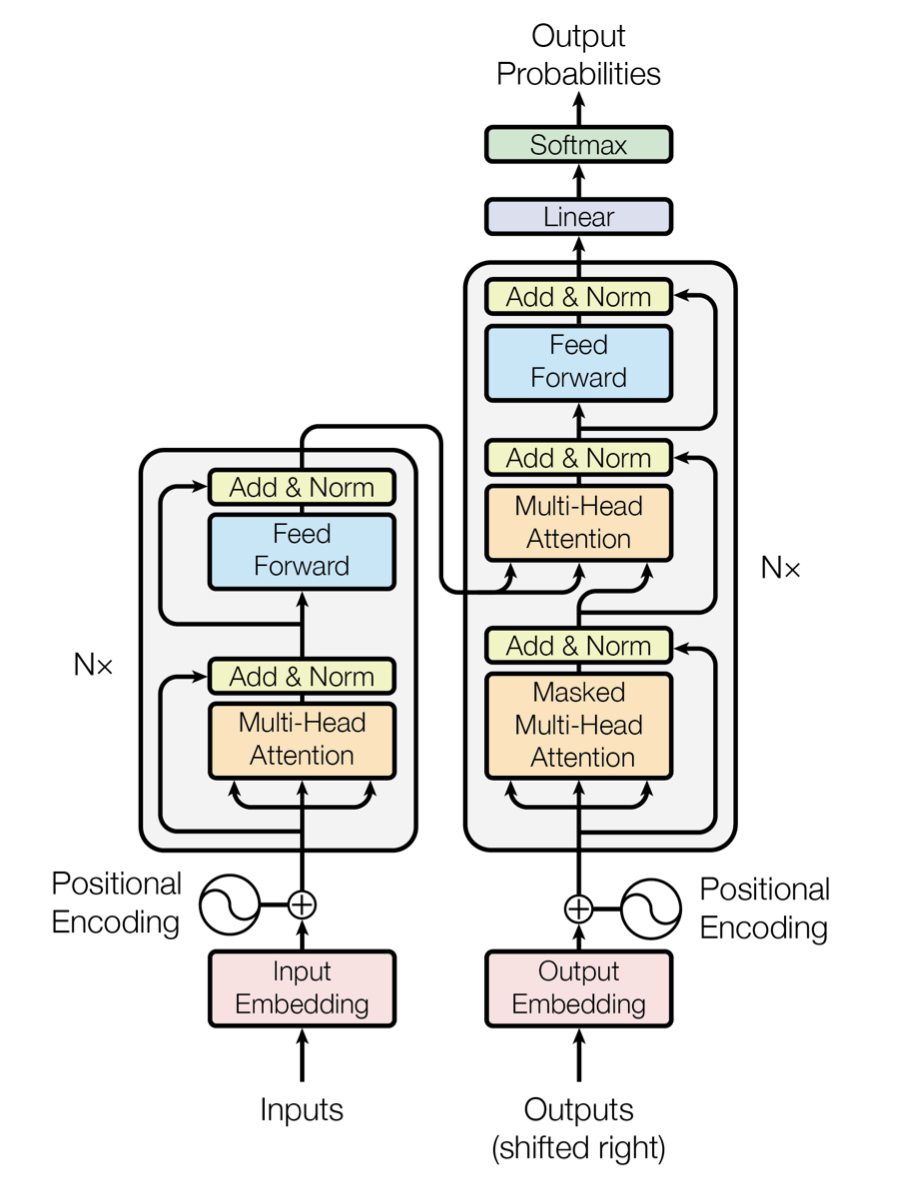
\includegraphics[width=0.5\textwidth]{figures/Transformer.png}
  \caption{Architecture of a Transformer model. \cite{Vaswani2023}}
  \label{fig:transformer}
\end{figure}

As already stated, a softmax function is used to get a probability distribution across all possible output tokens. Normally the sampling process of the next token is used to be a random process, where each tokens has the assigned weight from the softmax function. In order to increase or decrease randomness, a temperature parameter $T$ is introduced in the softmax function \cite{Peeperkorn2024}. For each output $z_i$ on token $t_i$ for a sequence with length $n$ the softmax function $softmax(\mathbf{z})_i$ with the temperature $T$ will be calculated as \cite{Peeperkorn2024}:

\begin{equation}
  softmax(\mathbf{z})_i = \frac{exp(\frac{z_i}{T})}{\sum^n_j exp(\frac{z_j}{T})}~~~where~\mathbf{z} \in \mathbb{R}^n.
\end{equation}

Increasing the temperature $T>1$ would lower high probabilities and increase low probabilities and therefore make the output more novel in theory. A temperatur $T<1$ would amplify high probabilities and make the text generation more predictable. Using a temperature $T=0$ change the generation to greedy sampling, as then only the token with the highest probability is used \cite{Peeperkorn2024}.

Todays top-tier like OpenAIs \ac{GPT} models or Metas \ac{LLaMA} models \acp{LM} do make use of the decoder part of the transformer \cite{Radford2018,Grattafiori2024}. Models especially with large amount of parameters are typically referred to as \acp{LLM}. Those decoder-only models do only have the target to make predictions for the token $t_i$. Those models use unsupervised pre-training, by using a text-corpora and maximizing the probabilities of each subsequent token in this corpora to be predicted. In former models like the original GPT version, after pre-training a task-specific supervised fine-tuning was necessary to get usable results \cite{Radford2018}.

The recent history of \acp{LM} showed, that increasing the corpora size on the pre-training and the parameters number enables the models to be able to process tasks from various domains without further fine-tuning \cite{Radford2018,Radford2019,Brown2020}. With the GPT-3 publication, \citet{Brown2020} showed that their model can leverage in-context learning to increase their performance on specific tasks. Therefore, in the input of the model, what is also called the prompt, examples will be added. For instance, when the \ac{LM} should process translation tasks, it get's in it's prompt examples like \textit{house $\rightarrow$ Haus} or \textit{light bulb $\rightarrow$ Glühbirne}. Including multiple examples is called few-shot prompting, while including one example is called one-shot-prompting and including no example is called zero-shot prompting.

This technique has shown great success especially when using larger models, as they were able to process in-context information more efficient. But also the zero-shot experiments showed superior performance to SOTA models in various tasks, showing the general capabilities of recent \acp{LM} \cite{Brown2020}. To enable this performance, \citet{Brown2020} used the Common Crawl corpora, filtered it and added also other smaller, but high quality corpora to their pre-training dataset. Therefore, the \ac{GPT}-3 pre-training dataset had access on over 500 billion tokens \cite{Brown2020}.

As the Common Crawl corpora follows the idea of providing a copy of the entire internet \cite{CCF2025} and other used corpora also provide prose text combined with the overall training goal of \acp{LM} leads to a superior performance in text generation but not in instruction following \cite{Ouyang2022}. In addition, \citet{Ouyang2022} states the real-world usage of \acp{LM} differ from the given corpora, as most users use instructions. Therefore, \ac{GPT}-3 was finetuned towards two datasets. One dataset uses human-given answers to prompts to fine-tune the model. In addition, human-labeled comparisons between answers of different \ac{GPT}-3 models are used to train a reward models, that is applied using reinforcement learning on the model. At the end of the experiements, the resulting InstructGPT model reached superior performance on human evaluated benchmarks based on the output on held-out prompts from customers. Even the smallest instruction tuned model with 1.3 billion parameters outperformed \ac{GPT}-3 with 175 billion parameters in this evaluation \cite{Ouyang2022}.

In order to choose ideal model for use-cases, on option could be to use benchmarks like MMLU-Pro \cite{Wang2024} or the human-evaluated Chatbot Arena \cite{Chiang2024}. The MMLU-Pro benchmark is testing for multi-task language understanding with the goal to test the various capabilities of LLMs. Therefore, the MMLU-Pro keeps tasks from maths, physics, law, engineering and various other topics \cite{Wang2024}. The Chatbot Arena\footnote{The Chatbot Arena can be accessed under \url{https://lmarena.ai}} is a live benchmark working with human preferences. Therefore, the use gets two answers from two distinct models to the user prompt. Then the human chooses which \ac{LM} performed better. Based on this feedback a win rate and a score can be calculated \cite{Chiang2024}.

The \acp{LLM} breakthrough performances on such benchmarks rely also on their high complexity. Models like GPT-3 are using 175B parameters make the use of multiple high-performance GPUs necessary \cite{Brown2020,Frantar2023}. There can be seen two methods how to utilise \acp{LLM} within a limited performance set up. First is to use smaller models with less parameters. This shows consequences in the abilities of the models \cite{Brown2020,Grattafiori2024}. Recent research shows that especially newer models can achieve prior state-of-the-art performance with less parameters \cite{Meta2024}.

Another way to use \acp{LLM} that fit into the limited configurations, but utilising large parameter models while handling a tradeoff with performance is quantisation. In general, quantisation methods lower the number of bits used per parameter. As naive quantisation leads to higher accuracy drops, methods like GPTQ or AWQ are developed. Both methods implement variants to lower the error, by either handling and lower the error in the quantisation process or by preserving salient weights. Both approaches show around 3x faster performance while producing high quality results compared to the standard 16-bit accuracy \cite{Frantar2023,Lin2024}.

In conclusion, \acp{LM} are \ac{ML} models consisting out of multiple multi-head attention and feed-forward network layers with the goal to predict the probability of a following token based on all previous tokens. Therefore, those models are designed as with a large amount of parameters and additional use pre-training based on large size corpora to achieve outperforming results. In the end, those models can be benchmarked using MMLU-Pro or the Chatbot Arena to test various capabilities of them.

\section{Sentence Embeddings}
\label{sec:sentence_embeddings}

Sentence embeddings in general have the idea to represent a text in a vector \cite{Singhal2001}. Building those vectors, the semantic of the sentence can be encoded in those embeddings, so that a meaningful similarity between the vectors can be calculated \cite{Reimers2019}. Typically this similarity is the cosine of the angle between two vectors, which is named cosine similarity. The property of the cosine function then allows, that the cosine between two vectors is 1.0 when they are total identical and 0.0 if not \cite{Singhal2001}. An visualisation of this behavior can be found in figure \ref{fig:cosine_similarity}. Such models are critical to enable large-scale semantic similarity comparisons which are useful for various use cases, like retrieving knowledge similar to a user query \cite{Reimers2019,Gao2024}.

\begin{figure}[t]
  \centering
  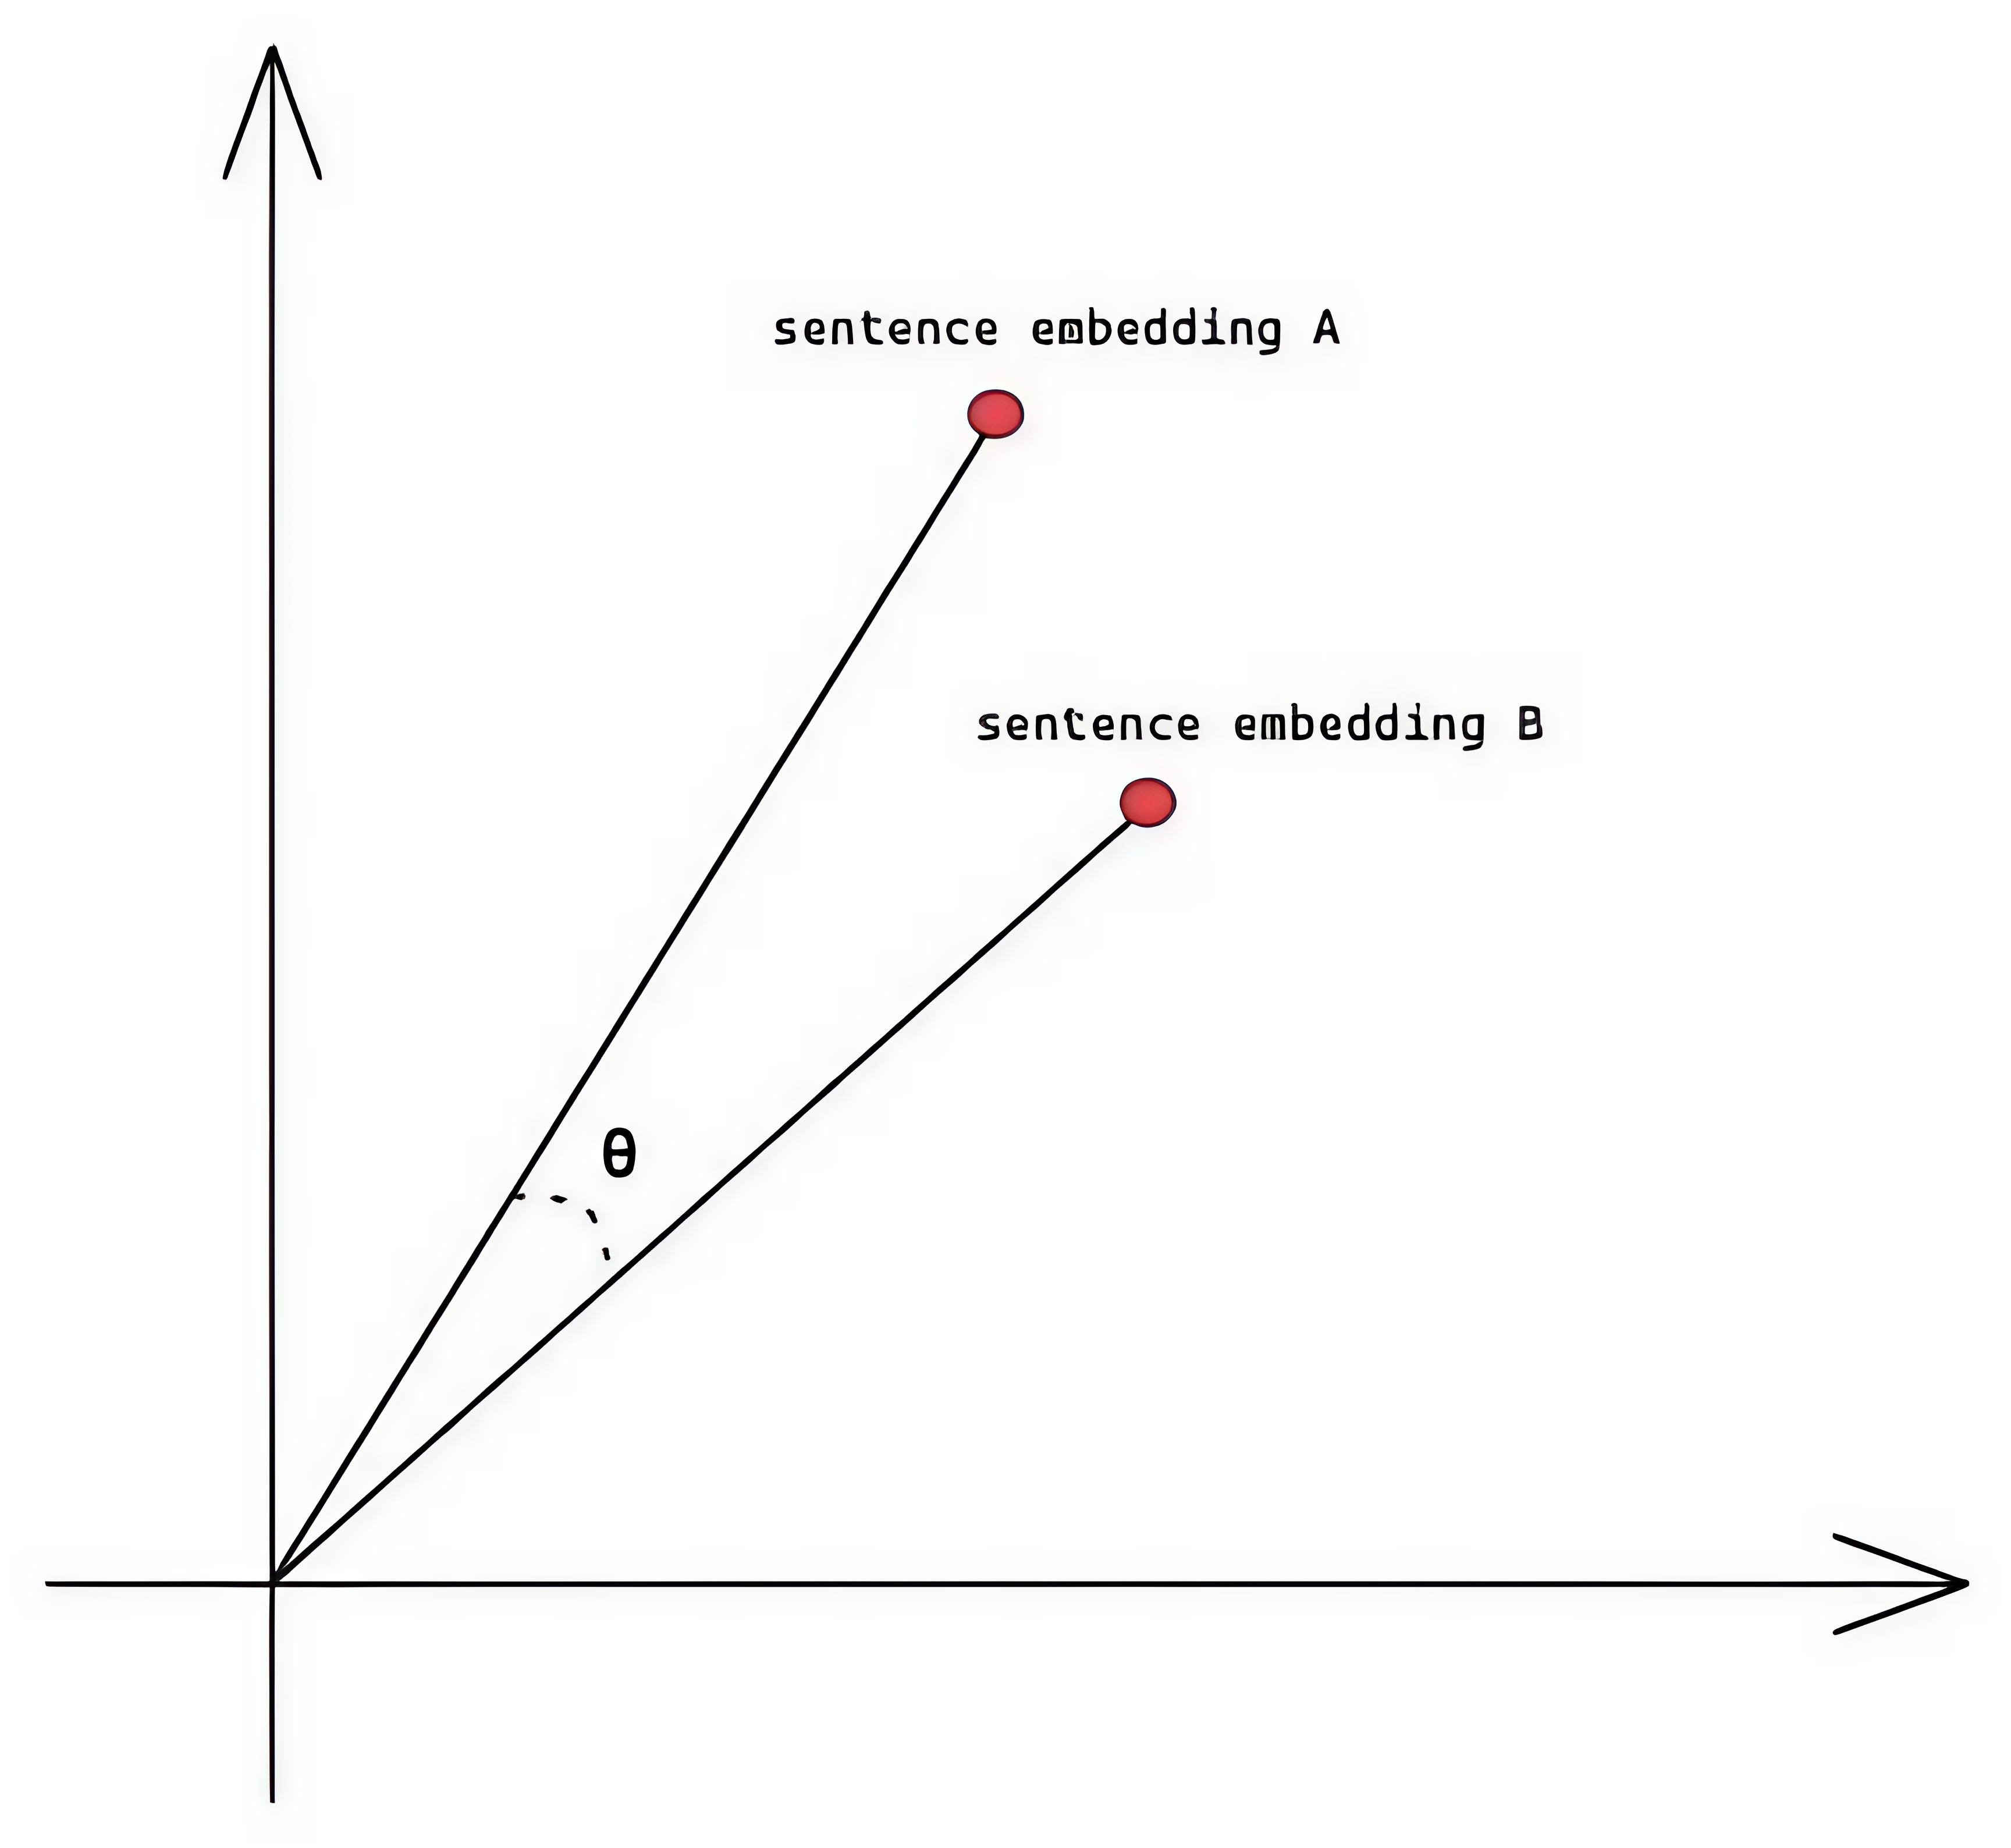
\includegraphics[width=0.6\textwidth]{figures/cosine_similarity.jpeg}
  \caption{Visualization of cosine similarity between two vectors showing how the angle between vectors determines their similarity score. \cite{Leys2022}}
  \label{fig:cosine_similarity}
\end{figure}

One recent model is M3-Embedding, which is trained to support semantic retrieval functions that rely on similarity functions. The overall idea of M3-Embedding is to support multiple languages, multiple retrieval functionalities and multiple input granularities. To achieve this goal M3-Embedding leverage the encoder architecture of transformers like stated in section \ref{sec:language_models} \cite{Chen2024}.

Training-wise, \citet{Chen2024} follows the pre-training approach, while fine-tuning later on high-quality data. The pre-training was done on unlabeled corpora utilising semantic structures like title-body or title-abstract. To support multi-linugua a translation dataset was leveraged. Then labeled corpora in different languages and synthesised corpora consisting of questions generated by \ac{GPT}-3.5 based on multilingual paragraphs were used to fine-tune the embeddings. Overall the M3-Embedding model was trained to detect if a queries matches a text passage from its semantics or not \cite{Chen2024}.

Overall sentence embeddings can be used to map sentence into the vector space, while also encoding semantic into this space. Leveraging vector algebra like the cosine similarity, semantic similarity between two sentence embeddings can be calculate. To achieve SOTA performance embeddings like M3-Embedding make use of the transformer architecture combined with extensive training sets and the pre-training technique.

\section{Retrieval Augmented Generation}
\label{sec:retrieval_augmented_generation}

As \acp{LM} are trained on large-size snapshots of corpora, they are by default not able to retrieve out-of-scope knowledge from the internal representation. Therefore, \ac{RAG} emerged as a solution to incorporate knowledge from external data sources into the \ac{LM} at runtime. \ac{RAG} in it's simplest form is build out of indexing, retrieval and generation. In the indexing step, the plain text, also called document, will be mapped into the vector space utilising embedding models like the previously named M3-Embeddings \cite{Gao2024}. This embeddings are stored for later retreive in a database that can handle vectors and vector algebra efficient \cite{Gao2024,Pan2024}.

\begin{figure}[t]
  \centering
  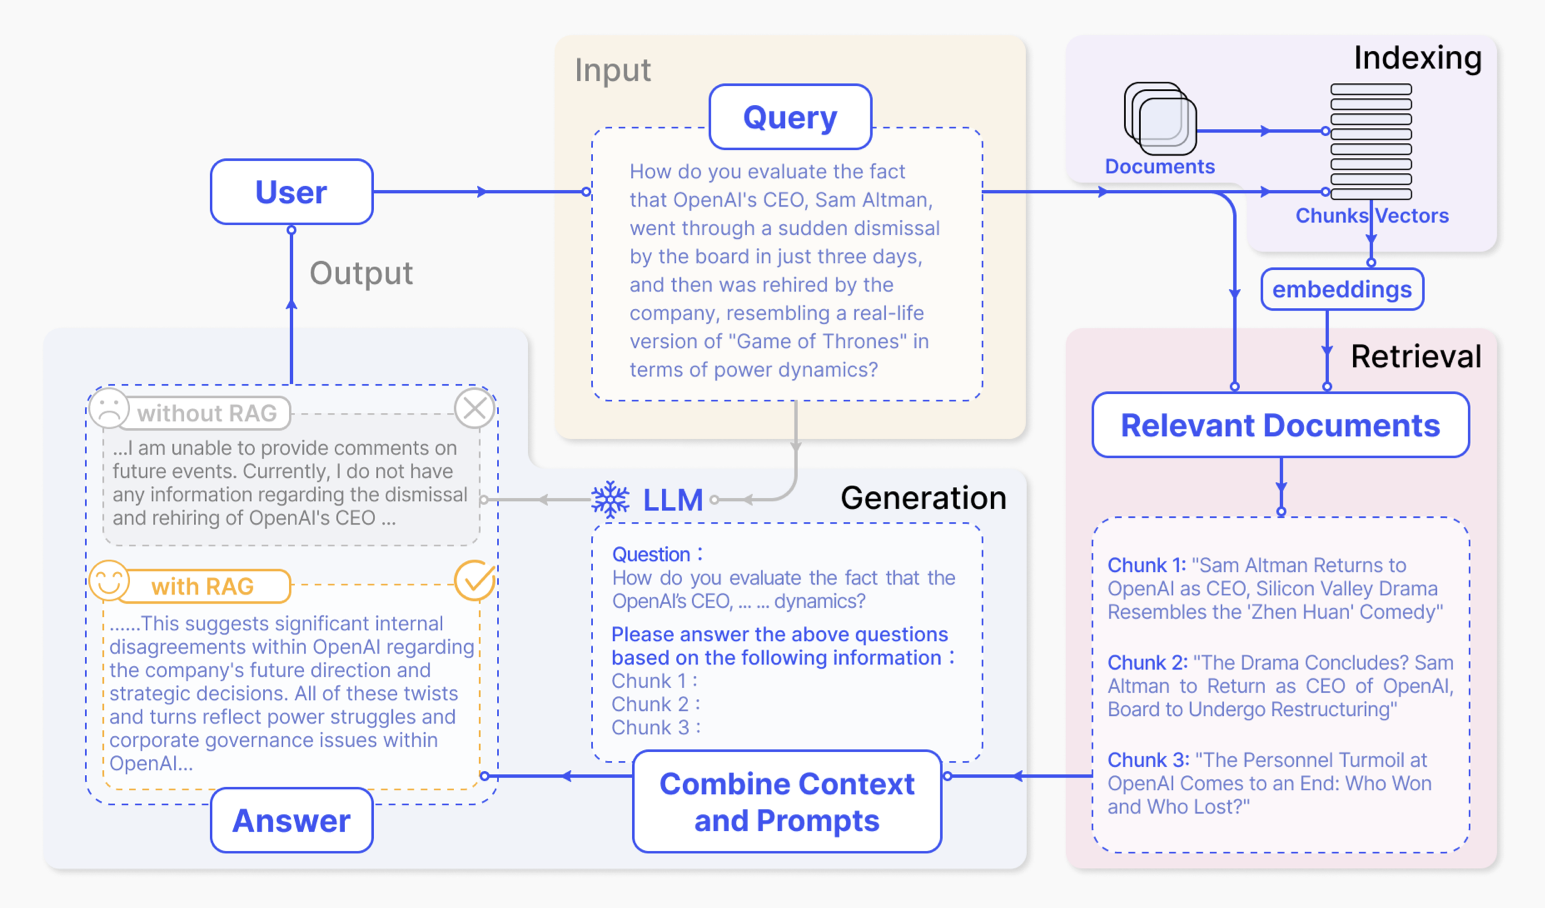
\includegraphics[width=0.8\textwidth]{figures/RAG.png}
  \caption{Overview of the Retrieval Augmented Generation (RAG) architecture showing the indexing, retrieval, and generation pipeline. \cite{Gao2024}}
  \label{fig:rag}
\end{figure}

In figure \ref{fig:rag} an overview about the steps and the functionality of each step can be found. The steps of retrieval and generation are done at runtime, whereas the indexing can run independend. The retrieval steps utilises again the embedding model to map the user query into the vector space. As shown in section \ref{sec:sentence_embeddings}, models like M3-Embeddings are trained on to calculate the similarity between documents and user queries. This enables the retrieval step to run a similarity search on the \ac{VDBMS} and retrieve the most relevant documents based on the user query. After the retrieval those documents can be composed into a prompt template, where additionaly to the user prompt, a system prompt can be defined. Then this prompt is send to the \ac{LM} with the goal to produce a external knowledge aware answer \cite{Gao2024}.

Besides the already explained embeddings the \ac{RAG} depends on a \ac{VDBMS}. Those databases consist like normal \ac{DBMS} out of a query processor and a storage manager. The query processor is optimising the query and processes especially the similarity searches. One example of \ac{VDBMS} is Qdrant. Qdrant uses filtering and vector set size depended execution paths. If a vector set, named collection in Qdrant, keeps many vectors, a brute-force search would be to extensive. Therefore, Qdrant would use pre-filtering mechanism that limit the search results and computations that have to be done. The storage manager manages the physical access and storage of the data \cite{Pan2024}.

As already stated Qdrant is an example for a \ac{VDBMS}. It uses the concept of collection, where vectors are stored that should be retrieved together, for instance to cluster vectors that all belong to one project. Additionally to the vectors, payloads can be used to store metadata alongside with the vectors. Qdrant offers a python client and a Langchain integration, which is useful to be leveraged in vector store projects \cite{Qdrant2025}. Langchain itself is a framework to develop application with \acp{LM} \cite{LangChain2025d}. Through its query optimisations, Qdrant is able to handle large-scale datasets efficient \cite{Qdrant2025,Pan2024}.

\ac{RAG} is one solution to integrate external knowledge bases, that can be updated efficient, into \acp{LM}. Therefore, \ac{RAG} makes use of the ability of embeddings to encode semantic similarity that can be retrieved using cosine similarity. In order to make use of \ac{RAG} the external knowledge bases have to be indexed using embeddings. To support \ac{RAG}, \ac{VDBMS} are utilised for an efficient indexing and retrieval process.

\section{AI Agents}
\label{sec:ai_agents}

\ac{AI} agents are a more narrow concept of a normal agent. \citet{Dorri2018} defines an agent as \enquote{(a)n entity which is placed in an environment and senses different parameters that are used to make a decision based on the goal of the entity. The entity performs the necessary action on the environment based on this decision.} \cite[S. 28574]{Dorri2018} The entity in this case is defined as the type of the agent. The enviroment is the place of the agent, which is defined by the accessibility and quality of data, predictability of outcomes, the dynamic of enviroment changes and continuity of the state. Parameters can be defined as the data that the agent gets and the action is the set of actions that the agent can take \cite{Dorri2018}.

Agents do have a decision engine. \ac{AI} agents typically narrow this decision engine nowadays down to \acp{LLM} \cite{Sapkota2025,Park2023}. Furthermore \ac{AI} agents are defined by having a high degree of idependence, while being task-specific and react and adapt to the current state \cite{Sapkota2025,OpenAI2025}. The high degree of independence differs to workflows, were the path how to achieve a goal is well-defined \cite{Anthropic2024}. The idea behind \acp{LLM} that power agents is to generate human-like behavior, as \acp{LLM} have internal representation of human behavior via the training data \cite{Park2023}.

To achieve this goal the agent architecture cosists of agent orchestration, a \ac{LLM} model used for decision making and reasoning and tools \cite{Wiesinger2025,OpenAI2025}. All components are executed by an agent runtime. The orchestration layer is the layer that defines which information an agent gets. This consists of managing memory, providing the prompt templates to the agent and define a message flow, so how the actions that the agent takes are executed \cite{Wiesinger2025}.

According to \citet{OpenAI2025} tools can be defined in three types: Data, Action, Orchestration. Data tools are concentrated on retrieving information from external systems. Therefore, data tools can query databases or search the web. Action tools enable the agent to take actions in external systems. This means, the agent could update or create record in systems like a \ac{CRM}. Orchestration agents, agents that serve themselve as tools. This concept is referred to as \ac{MAS} an will be explained in detail in section \ref{sec:multi_agent_systems}. In general, tools are an enabler to AI agent to directly interact with external systems. This interaction allows \ac{AI} agents to act highly idenpendent.

A single \ac{AI} agent is targeted to process a single well defined tasks together with defined tools. Within this task it stays indepent, but a single \ac{AI} agent is not offering a high degree of flexibility, when not using other agents as tools \cite{Sapkota2025}. In this use case \citet{Anthropic2024} proposes that \ac{AI} agents are able to understand complex inputs, can make use of tools in reliable manner and recover from errors. In addition, \ac{AI} agents can engage in reasoning and planning over given tasks \cite{Anthropic2024}.

The ability to reason is especially used in the ReAct agent framework proposed by \citet{Yao2023}. The idea behind the ReAct frame is the synergy between reasoning on perceptions and taking action from there on, as this is a typical learning behavior of humans. In the proposed idea, the \ac{LLM} is mocking this human behavior by being told to reason and act \cite{Yao2023}.

In general the ReAct framework prompts an \ac{LLM} to reason about a task using a defined state. The resulting thought will be written in the state, alongside with all following thought. Besides giving a thought, the \ac{LLM} is prompted to take an action which could either be running a tool, running itself again or ending the process. This action leads to a result which is called observation. After each thought in the state, an action and the following observation is stored. Together this build up a history, that the \ac{LLM} could leverage to memorise it's own thoughts and actions \cite{Yao2023}.

To implement \ac{AI} agents \citet{Anthropic2024} proposes to take a framework like LangGraph. LangGraph is an open-source frame to build agent with the whole agent ecosystem. Therefore, tools, memory and the state can be define either using LangGraph in python or JavaScript. LangGraph offers a high extensibility, to define the agent as individual as needed \cite{LangChain2025}. Alltogether LangGraph is integrated with the LangChain package \cite{LangChain2025a}.

Single agents bring challenges along. First of all there are limitations brought by the \ac{LLM}, which is about missing the understanding for causal relationships. This arises out of the goal to generate text instead of detection causal relationships. In addition, as \acp{LLM} are prompt sensitive, the overall outcome is prompt sensitve \cite{Sapkota2025}. Furthermore, \citet{Sapkota2025} states, that \ac{AI} agents have limited long-horizon planning and missing recovery mechanism leading them to get stuck in a loop.

Overall \ac{AI} agents are defined by a model taking independent actions. Therefore, an agent must be orchestrated and has access to various tools. The ReAct framework can implement the ideas and capabilities of \ac{AI} agents so that the \acp{LLM} behave human-like and therefore achieve good results.

\section{Multi-Agent-Systems}
\label{sec:multi_agent_systems}

As stated in the previous section agents are often limited to a single task, being unflexible to solve other tasks. A solution to this limitation can be found in \ac{MAS}. The idea behind them is to produce a cost efficient, flexible and reliable solution, by using multiple agents instead of one. Therefore, the complex task can be splitted into multile simple task. The theory is that the simpler task lead to lower cost solutions amortising the overhead produced to manage the \ac{MAS} \cite{Dorri2018}.

So to make a general \ac{MAS} work, agents are defined for various simpler task. In addition, multiple agents could be defined for the same task. Then the routing within the \ac{MAS} must be defined. This means, that there is either a static or dynamic topology of agent and the communication routes between them. In this topology there coould a leader agent, that defines the actions that have to be taken by other agents and they communicate solely to the leader. The second option is a leaderless \ac{MAS}, where each agent decide on its on which agent is to call next \cite{Dorri2018}.

Especially leaderless \ac{MAS} bring a high degree of flexibility with them. From this, a high complexity arises in coordinating the agents towards one shared goal, organising the agents to communicate to each other and allocating a task to the correct agent with the correct inputs. Additionally, as multiple agents conduct to one goal, fault propagation and fault detection is getting more complex \cite{Dorri2018}.

All mentioned points can also be mapped and extended when focussing on \ac{LLM} based \ac{MAS}. In general, due to the capabilities of \acp{LLM}, single \ac{AI} agents are already able to take care of complex tasks. But the only way to keep with more complex task is to increase instruction size and the number of tools, which could lead the \ac{AI} agents into failing or looping like already outlined in section \ref{sec:ai_agents} \cite{OpenAI2025}. Therefore, the goal decomposition into various specialised \ac{AI} agents remains also a key enable to solve more complex tasks \cite{Sapkota2025}.

In the case of \ac{LLM}-based \ac{MAS}, each agent is in general required the same building blocks like mentioned in section \ref{sec:ai_agents}. This concept is adapted to \ac{MAS} by extending the state to a shared state \cite{Sapkota2025}. In addition, each agent in a \ac{MAS} needs to have an handoff. This handoff is defined by the agent itself and decides the further flow within agent system. Especially in LangGraph the handoff specifies the destination of the handoff, so the next tool or agent, and the payload, meaning the update of a state or inputs to the next agent or tool. The state itself in LangGraph is a python dictonary with pre-defined fields. Therefore, the orchestration layer of the \ac{LLM}-based \ac{MAS} gets more complex, what could be handled by frameworks like LangGraph \cite{LangChain2025b}.

The agentic architecture patterns of a \ac{LLM}-based \ac{MAS} follows the classic \ac{MAS} patterns as depicted in figure \ref{fig:mas_architecture}.

\begin{figure}[t]
  \centering
  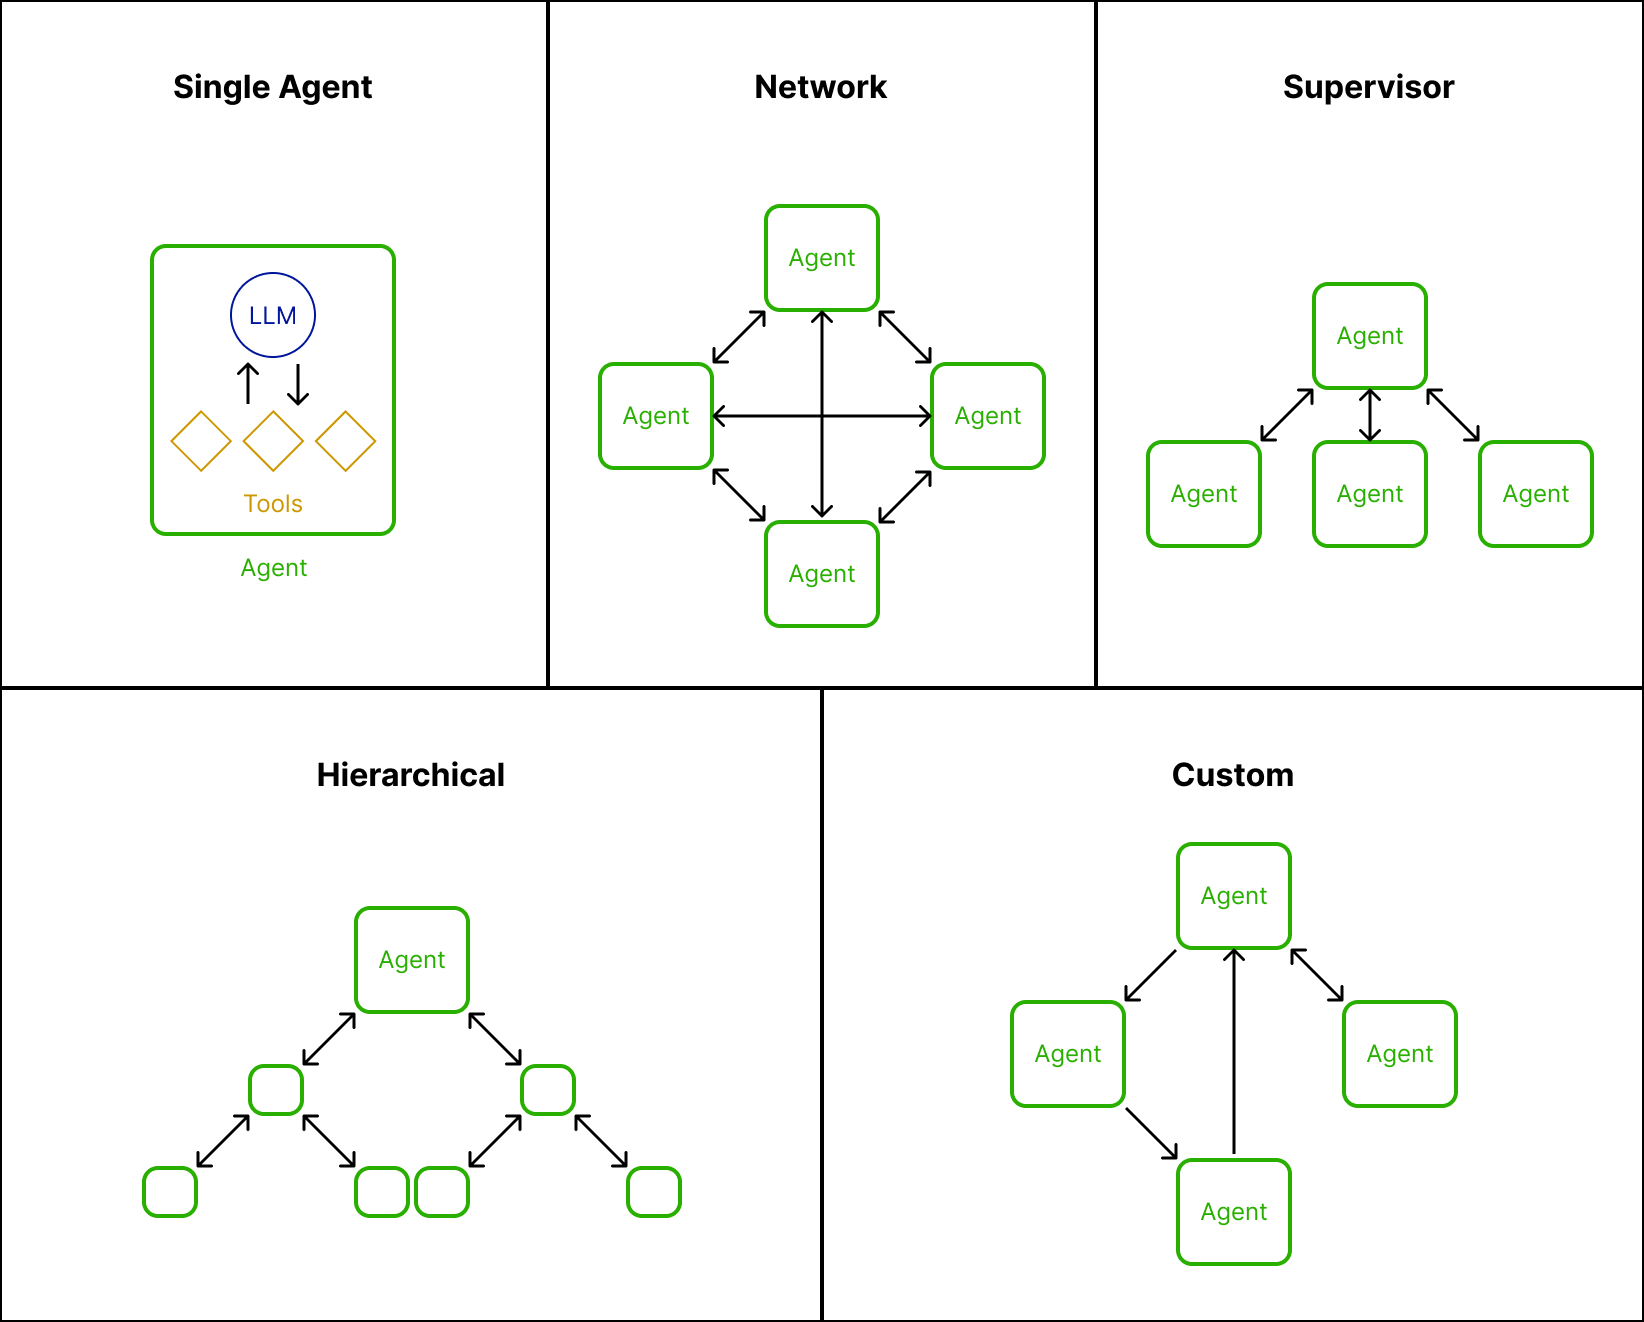
\includegraphics[width=0.8\textwidth]{figures/Multi-agent architectures.png}
  \caption{Example multi-agent architecture patterns showing supervisor, hierarchical, network, and custom patterns for LLM-based multi-agent systems (self-created after \cite{LangChain2025b})}
  \label{fig:mas_architecture}
\end{figure}

The leader-follow pattern is defined as supervisor pattern by \citet{LangChain2025b}, alongside with the hierarchical pattern. The supervisor pattern therefore, has on supervisor agents, that manages the communication to other expert agents, which themselve can only communicate with the supervisor agent. In the hierarchical pattern, those expert agent can itself be supervisors to other expert agents \cite{LangChain2025b}.

\ac{LLM}-based \ac{MAS} can also be used with decentralised leaderless architecture \cite{OpenAI2025,LangChain2025b}. This concept is extended by \citet{LangChain2025b} to network and custom patterns. The network pattern allows each agent to decide to which agent in the network it should handoff its request. In this pattern each agent controls the flow within the \ac{MAS} \cite{LangChain2025b,OpenAI2025}. The custom pattern could not be perfectly adapted to either leader-follow nor leaderless patterns. In the custom pattern a user can also define workflows for specific agents or let some agents not communicate with specified other agents \cite{LangChain2025b}. The big benefit besides the theoretical more accurate performance of \ac{LLM}-based \ac{MAS}, is the high modularity that is being enabled. In addition, through packages like LangGraph, the communication flow between the agents can be precisely defined alongside with the agents specialisation \cite{LangChain2025b}.

Nevertheless, \ac{LLM}-based \ac{MAS} amplifies and adds challenges that were already apparent with \ac{AI} agents. At first within \ac{LLM}-based \ac{MAS} the lack of causal understanding gets amplified, as agents have to run multiple times. Each \ac{AI} agent brings already uncertainty with them, especially being prompt sensitive and are vulnerable to infinite loops. Using multiple \ac{AI} agents, leads to even more uncertainty and robustness \cite{Sapkota2025}. In addition, the communication and coordination of \ac{LLM}-based \ac{MAS} reveals further bottlenecks. This is amplified by the fact, that \acp{LLM} have limited context length model-wise and infrastructure-wise \cite{Kwon2023}. This adds complexity in managing shared context and aligning on one goal \cite{Sapkota2025,Han2025}. As \acp{LLM} can produce unpredicted behavior, \ac{LLM}-based \ac{MAS} is non-composable. This means, that adding another \ac{AI} agent to a \ac{LLM}-based \ac{MAS} could lead to more complexity in the prompts, but it does not necessarily mean, that this new agent is used. Therefore, new agents could decrease the overall performance of the \ac{MAS}. In addtion, with further scaling and the prompt senstivity of \acp{LLM} it remains complex to detect the root causes of issues in the \ac{MAS}. An evolving challenge is the immature foundations and the reletavely new reasearch field aroun \acp{LLM} in general, but especially in \ac{AI} agents and \ac{LLM}-based \ac{MAS} \cite{Sapkota2025}.

As this research subject is rapidly evolving, also solutions are already found towards several problems. For instance to support \acp{LLM} in better reasoning, one way is to include external knowledge bases using \ac{RAG}. In addition, as a \ac{LLM}-based \ac{MAS} also use \ac{AI} agents, those agent can also access tools, which are deterministic and deliver reliable results. The root cause tracing issue can be solved by using monitoring and auditing tools. In order to give \acp{LLM} a way to sense causality by using complex simulation-tools. The communication bottlenecks can also be solved using different memory architectures \cite{Sapkota2025}.

Overall \ac{LLM}-based \ac{MAS} are one solution to solve complex problems efficient and accurate. Therefore, multiple \ac{AI} agents, that solve one piece of the overall problem, can communicate and take action. This could be done within a network of \ac{AI} agents, hierarchical solutions or fully custom solutions. Nevertheless, as the overhead increases and so does the \ac{LLM} calls, \ac{LLM}-based \ac{MAS} are vulnerable to challenges like uncertainty amplification or tracibility issues. As the research field is relatively new, also several solutions like tracibility tooling or uncertainty reduction by external knowledge and tool use evolved.

\section{Agent Design}
\label{sec:agent_design}

As the area of \ac{AI} agent research evolves, so does the research about best practises about when to use \ac{AI} agents and how to design them. In general, \citet{OpenAI2025} recommends to use \ac{AI} agents as soon as  deterministic rules fall short. This includes especially, if a problem can not be put into a ruleset straightforward. Especially if the decision making within the problem is additionally complex and the problem relies mainly on unstructured data, \ac{AI} agents are proposed to outperform other approaches \cite{OpenAI2025}.

As already stated in section \ref{sec:ai_agents}, \ac{AI} agents are in general bound to one single task and also limited in the amount of context they can handle. Such cases can be detected, if the agents are starting to fail following instructions or the decision making performance starts to worsen. By design, some problems can lead to complex context and a higher amount of tools, which itself can lead to tool overload. In this case, the context, tasks and following this also the tools per agent can be splitted down to \ac{MAS}. In addition, complex problems can also require complex logic which would be preferable be splitted down into several subtasks using \ac{MAS} \cite{OpenAI2025,LangChain2025b}. Nevertheless, \ac{LLM}-based \ac{MAS} has to be design efficient, as this architecture comes with high costs \cite{Hadfield2025}.

On the overall agent design \citet{Anthropic2024} recommends simplicity before complexity. Furthermore, they define agent systems as a tradeoff between latency and overall task performance. In general, \citet{Hadfield2025} proposes to design an agentic system like a human team. This is followed by keeping the tasks consise and define clear actions \cite{OpenAI2025}. Furthermore, the context should stay human-understandable, as \acp{LLM} are trained on human content \cite{Anthropic2024}. In addition, \citet{Hadfield2025} recommends to use compression of the context, to keep the context shorter and more understandable. In general all of this comes down to the hypothesis created by \citet{Anthropic2024}, if a human can solve a task and \ac{AI} agent or \ac{LLM} should also be able to solve it. But also, \citet{Anthropic2024} follows up, that the problems and prompts should be kept obvious to solve. In addition, \citet{OpenAI2025} recommends to capture edge cases in order to make the \ac{AI} agents more robust overall. Specifically on \ac{LLM}-based \ac{MAS}, \citet{OpenAI2025} recommends to keep the single components flexible and composable.

As \ac{LLM}-based \ac{MAS} do have \acp{LLM} as decision engine and as already outline those models reamin prompt sensitive, prompt engineering remains critical to challenges in such \ac{MAS} \cite{OpenAI2025}. First of all, \citet{Anthropic2024} recommends to think about the training content and intentions of \acp{LM}. Those models were trained mainly on prose text and are created to generate text. That is why, \citet{Anthropic2024} recommends to keep the prompt format, but also the output format as close to the training data as possible. Following this recommendation no formatting overheads lowering the performance of the \ac{MAS} should be included by design. In addition, \citet{Hadfield2025} proposes to teach the \ac{AI} agents how to orchestrate the \ac{MAS}. This also includes to guide the thinking process of the \ac{AI} agents \cite{Anthropic2024}. Overall the \ac{AI} are recommended to perform better, if the prompts are kept clear and structured \cite{OpenAI2025}.

As already outlined in section \ref{sec:language_models} one apparent technique to produce high quality prompts is to leverage in-context learning. When building in-context learning enabled prompts by using either few-shot or one-shot prompting, decisions have to be made about the examples \cite{Schulhoff2025}. \citet{Schulhoff2025} outlines the quantity, ordering, format and similarity as decisive points. Already before providing examples the prompt can be designed proper \cite{Schulhoff2025}. Therefore, \citet{Schulhoff2025} outlines different styles of prompting, including role, style or emotion prompting. Another proposed prompt technique is \ac{CoT}. In \ac{CoT} prompting, the \ac{LLM} gets provocated to think step by step through the tasks. In addition, few-shot \ac{CoT} includes \ac{CoT} examples in the prompt. In addtion, automatic prompt optimisation can be used to improve the performance of the \ac{AI} agents in the \ac{MAS} \cite{Schulhoff2025}.

\citet{Schulhoff2025} experimented multiple configurations with zero-shot and few-shot prompting against the MMLU benchmark, which is similar to the MMLU-Pro benchmark showed in section \ref{sec:language_models}. Within this experiment the few-shot \ac{CoT} prompting is the worst, while the few-shot \ac{CoT} prompt worked the best. Therefore, \citet{Schulhoff2025} agrees with the earlier result of \citet{Brown2020}, which outlined \acp{LM} as few-shot learners.

In addition to the prompt itself, the definition of useful tools is crucial to solve specific tasks that have to make use of external applications or knowledge \cite{OpenAI2025}. As the tools itself have to be described in the prompt, the tool description have to be as good engineered as the overall prompt accordings to \citet{Anthropic2024}. In addition, tools have to be tested extensive, as their is a structured handoff, that has to be generated out of an unstructured text using a \ac{LLM} \cite{Anthropic2024}. Therefore, \citet{Anthropic2024} advises to test and log how tools are used. By further iterating, it is recommended to design prompts simpler \cite{Anthropic2024}. Following this recommendation, tools could also be made fool-proof by design, so that it is harder for the \ac{LLM} to make a mistake.

After designing the agents, the iteration for better performance is to trace and evaluate the agents. \citet{Hadfield2025} proposes therefore to start immediately after designing \ac{AI} agents using small examples. In addition, it is proposed that human evaluation should be used to keep track of errors, that are not apparent in automation. Therefore the agent execution, but especially the tool execution should be traced and later on debugged \cite{Hadfield2025}. One example platform for this kind of \ac{LLM} engineering is Langfuse \cite{Inc.2025}.

Overall, as \acp{LLM} come with limitation and challenges, it is crucial to design \ac{AI} agents using \acp{LLM} as their decision making engine proper. This includes the general approach to design \ac{AI} agents and the \ac{LLM}-based \ac{MAS} as human-like tasks for a single or for multiple specialised. Combined with proper prompt and tool engineering, \ac{LLM}-based \ac{MAS} could excel on complex tasks \cite{Hadfield2025}.

\chapter{Related Work}
\label{ch:related_work_chapter}

In this section the goal is to show the current state-of-the-art training and benchmarking datasets alongside various approaches in the field of information extraction with a focus on solutions in the are of closed information extraction. Therefore, REBEL as one of the first large scale datasets for open and closed information extraction followed by synthIE, a datasets which is synthecially generated using models of the GPT-3.5 will be shown in section \ref{sec:related_datasets}. In the following section \ref{sec:related_approaches}, the various approaches ranging from transformer fine-tuning over prompt-tuning towards use of \ac{AI} agent for the problem of open and closed information extraction will be shown.

\section{Related Datasets}
\label{sec:related_datasets}

The datasets remain crucial to train, but especially to evaluate approaches in the area of closed-information extraction correct. This implies a high quality, but also high volume dataset \cite{Josifoski2023}. Therefore, the REBEL dataset was conducted by analysing Wikipedia Abstracts and extract all Hyperlinks out of that. In addtion a RoBERTa \ac{LM} is used to filter whether a text contains the extracted triples by leveraging the entailment prediction of RoBERTa. This results in a large scale dataset, where noise is accepted and which is automatically created. Therefore, the REBEL dataset can be defined as a silver-standard dataset. As the REBEL dataset also contains the \acp{URI} for the extracted entities and predicates, it can be used for relation extraction as well as for closed information extraction \cite{HuguetCabot2021}.

Following up on the problems of the REBEL dataset being noisy and skewed in terms of predicate frequency, the advances in the field of \acp{LM} \citet{Josifoski2023} introduced the synthIE dataset. The idea is to leverage the advances in text generation that a \ac{LM} from the GPT-3.5 series has and generating the text correlated to the expected triples \cite{Josifoski2023}. Following this idea, \citet{Josifoski2023} creates a unskewed set of triples based on a subset of wikidata and than prompting the triples with an corresponding instruction into text-davinci-003, which is based on InstructGPT, or code-davinci-002, which is a base GPT model \cite{Josifoski2023,OpenAI2025a}. Human annotated samples showed, that in contrast to REBEL most of the triples within the text generated by the synthIE dataset approach were detectable \cite{Josifoski2023}.

Overall, \citet{HuguetCabot2021} and \cite{Josifoski2023} provided large scale datasets. The synthIE dataset remains of higher quality and therefore promises better results when used for evaluation. Both datasets are providing large amounts of training, validation and testing data, providing a foundation for approach development in the area of closed information extraction.

\section{Related Approaches}
\label{sec:related_approaches}

Like already outline in section \ref{sec:closed_information_extraction} the area of open and closed information extraction have the research streams of pipeline- and joint-approaches. Both streams relied on a broad variety of solutions ranging from table-filling with tag probability learning over LSTM-based approaches to encoder-decoder models \cite{Zhang2022,Angeli2015,Trisedya2019}. With current advances of Seq2Seq text generation models towards the transformer architecture, recent approaches mainly implement various kinds of transformers in their solution architectures \cite{Josifoski2021,Josifoski2023,Moeller2024}.

Earlier implementations prior to the emergence of \acp{LLM} showed already superior performance using transformers to other state-of-the-art solutions. One example for this is the REBEL approach \cite{HuguetCabot2021}. Leveraging a large dataset of texts as queries and triples as outputs, the BERT-model fine-tuned by \citet{HuguetCabot2021} surpassed every compared method on similar benchmarking datasets, presenting a flexible relation extraction model.

\citet{Josifoski2021} introduced the idea of GenIE, which is adapting the idea of REBEL towards closed information extraction. This especially meant that the decoding in the BART \ac{LM} was constrained towards the underlying knowledge base, which is Wikidata \cite{Josifoski2021}. Therefore, \citet{Josifoski2021} used an output linearization by introducing special tokens to delimit subject, predicate and object. In addition, \cite{Josifoski2021} introduced a constrained beam search, that limits which tokens can be generated towards Wikidata. This idea on how to secure valid triple generation, outperformed the state-of-the-art pipeline consisting of named entity recognition, entity disambiguation, relation classification and triplet classification when released \cite{Josifoski2021}.

Using the idea of GenIE and the quality of the synthIE dataset, \citet{Josifoski2023} introduced the synthIE model. The synthIE model follows the architecture of GenIE, but replaces BERT by Flan-T5 \ac{LM} due to a higher availablity of usable pre-training configurations. The results showed, that the best synthIE model trained on the train split of synthIE dataset could surpass the REBEL-trained GenIE model, which was also using Flan-T5 in this comparison, by a gap of over 0.8 macro-F1 using the synthIE-text dataset. This outlined the high correlation between the training and benchmarking dataset quality and the overall quality on the model \cite{Josifoski2023}.

Proceeding on to ideas of leveraging foundation models that then can be either fine-tuned or prompt engineered, \citet{Xue2024} presented a pipeline approach with fine-tuned \acp{LLM} for Relation Extraction, Subject Identification and Triplet Fact Extraction, while \citet{Chen2024} presented a prompt tuning approach for joint optimisation. The approach of \citet{Xue2024} was evaluated on the document-relation extraction dataset Re-DocRED showing a 10\% increase in F1-score compared to state-of-the-art models. Furthermore, it was shown that non fine-tuned models like the base ChatGPT model were outperformed by a large gap \cite{Xue2024}.

The approach of \citet{Chen2024} showed the opposite, while proposing prompt tuning as technique to adapt \acp{LM} towards an open information extraction task. In difference to \citet{Xue2024} the relation were extracted among sentences instead of whole documents. The results showed, that using intelligent prompt tuning approaches can match state-of-the-art performance compared to open information extraction fine-tuning approaches. It has to be noticed, that \citet{Chen2024} as well as \cite{Xue2024} used different datasets than \citet{Josifoski2023} which limits the implications on the closed information extraction problem, but remains relevant for the overall approach in the field of information extraction.

The most similar approach to this work remains AgentRE from \citet{Shi2024}. In remarks of advances in using \ac{AI} agents, \citet{Shi2024} proposed a single-agent solution to open information extraction. This agent had access to a retrieval module and a memory module. The retrieval module was able to provide relevant samples and context from an existing knowledge graph. This included retrieving sample triples as well as relation descriptions. The memory module followed the idea of saving incorrect and correct triples extractions, while including the \ac{LLM} to process on self-reflection. The agent itself was in charge of making use of the modules, while also extracting the correct triples out of the given text \cite{Shi2024}.

This approach was tested against various different approaches on benchmarking data-sets that are non-related to datasets like REBEL or synthIE. Especially the used english dataset named SciERC, can be defined as rather limited and old \cite{Luan2018}. The experiments were conducted on GPT-3.5 Turbo and on a reasoning trajectory fine-tuned Llama-2-7B. The AgentRE approach outperformed the compared approaches on a majority of the datasets, showing the ability of \ac{AI} agents to tackle information extraction \cite{Shi2024}. As previously stated, the implications on closed information extraction remains limited also for this approach.

The related work shows, that apparent advances in \ac{LLM} reasearch can also advance results in open and closed information extraction. It has been shown that various approaches from fine-tuning over prompt-tuning to agent-frameworks can handle the subject of information extraction. Even more has been shown, that high quality dataset are crucial to train and especially benchmark models for closed-information extraction. Many of the outlined approaches are not including the advances of the most recent \acp{LLM} or do not work on the closed-information extraction and are therefore the results are not fully applicable on this work.

\chapter{Approach}
\label{ch:approach}

This work introduce a novel approach to closed information extraction using multi-agent systems. The overall idea is evaluate both the pipeline and joint approach to closed information extraction conducted by multiple specialised agents. In order to fullfil the task the agents should be able to access and retrieve data from the knowledge graph directly. Therefore the concept of tools should be utilised.

The general design follows to goal to achieve an multi-agent system that can be applied to real-world usage and therefore can handle various type of texts and extract triples out of them. This is why, the approach relies solely on prompt tuning and in-context learning rather than on fine-tuning models. The concept of limiting to in-context learning is based on \citet{Brown2020} achieving outperformance with in-context learning against other domain fine-tuned models. Additionally, recent advances of various \acp{LLM} to outperform prior models by a huge marging or match the performance of prior models while keeping lower parameter sizes \cite{MetaAI2025,Chiang2024} shows increased capabilities and can imply higher in-context learning abilities. The exact advances will be outlined in section \ref{sec:eval_language_models}.

This work followed an iterative approach in designing various multi-agent systems following the agent design best practises shown in section \ref{sec:agent_design}. As of my knowledge, there is no other work proposed using the multi-agent system approach to closed information extraction, which makes the iterative approach crucial. This approach is giving the ability to learn the limitations of the agents and then iterate with those ideas. From the output four core architecture arose. The baseline (section \ref{subsec:baseline}) structure following strictly the closed pipeline idea. The supervisor (section \ref{subsec:supervisor}) architecture splitting up tasks from the baseline. The ReAct architecture (section \ref{subsec:react}) as the opposite direction is simplifying all agents to one, while keeping the tools. The full network system (section \ref{subsec:network}) shows the abilities of having expert agents that are defining the flow through the agent system themselves.

In addition to the agents, multiple tools arose with the most important tool to fulfill the closed information extraction being the URI retrieval tool (section \ref{subsec:uri_retrieval}), which is designed to match search terms to URIs. To increase the knowledge graph incorporation, the tools of a network traversal search (section \ref{subsec:network_traversal}), a semantic validation (section \ref{subsec:semantic_validation}) and a turtle to label tool (section \ref{subsec:turtle_to_label}) were developed. Meaning that those tools have been developed does not imply that each architecture was connected to each tool.

The agents are designed as \ac{LLM} calls with a prompt template that is field with selected fields from the prompt. In theory, more and more \acp{LLM} in LangChain support structured output, meaning that the output of the \ac{LLM} is mapped automatically to a pre-defined scheme \cite{LangChain2025e}. As this structured output experienced as not supported by all models, this work relies on parsing instructions out of the text generation of the \acp{LLM} directly. This is done by requesting the \ac{LLM} to output specific XML-tags with information of the next agent, the final output, the instruction for the next agent or the tool input.

In addition, it has to be mentioned that all architectures were further advanced in regards of prompts and tools through the process, but especially those that were achieving the best results. As already stated, the process were imperative and so was the tool development, meaning that some tools were only developed for specific architectures. Further details which tools were evaluated for which architectures can be found in section \ref{sec:evaluation_configurations}.

\section{Agent Architectures}
\label{sec:agent_architectures}

In the following section the various agent architectures will be outlined. This is including the declaration which agents have been used and how the overall flow is desing. In addition the definition of the state and handoff will be shown per architecture.

\subsection{Baseline Architecture}
\label{subsec:baseline}

\begin{figure}[h]
  \centering
  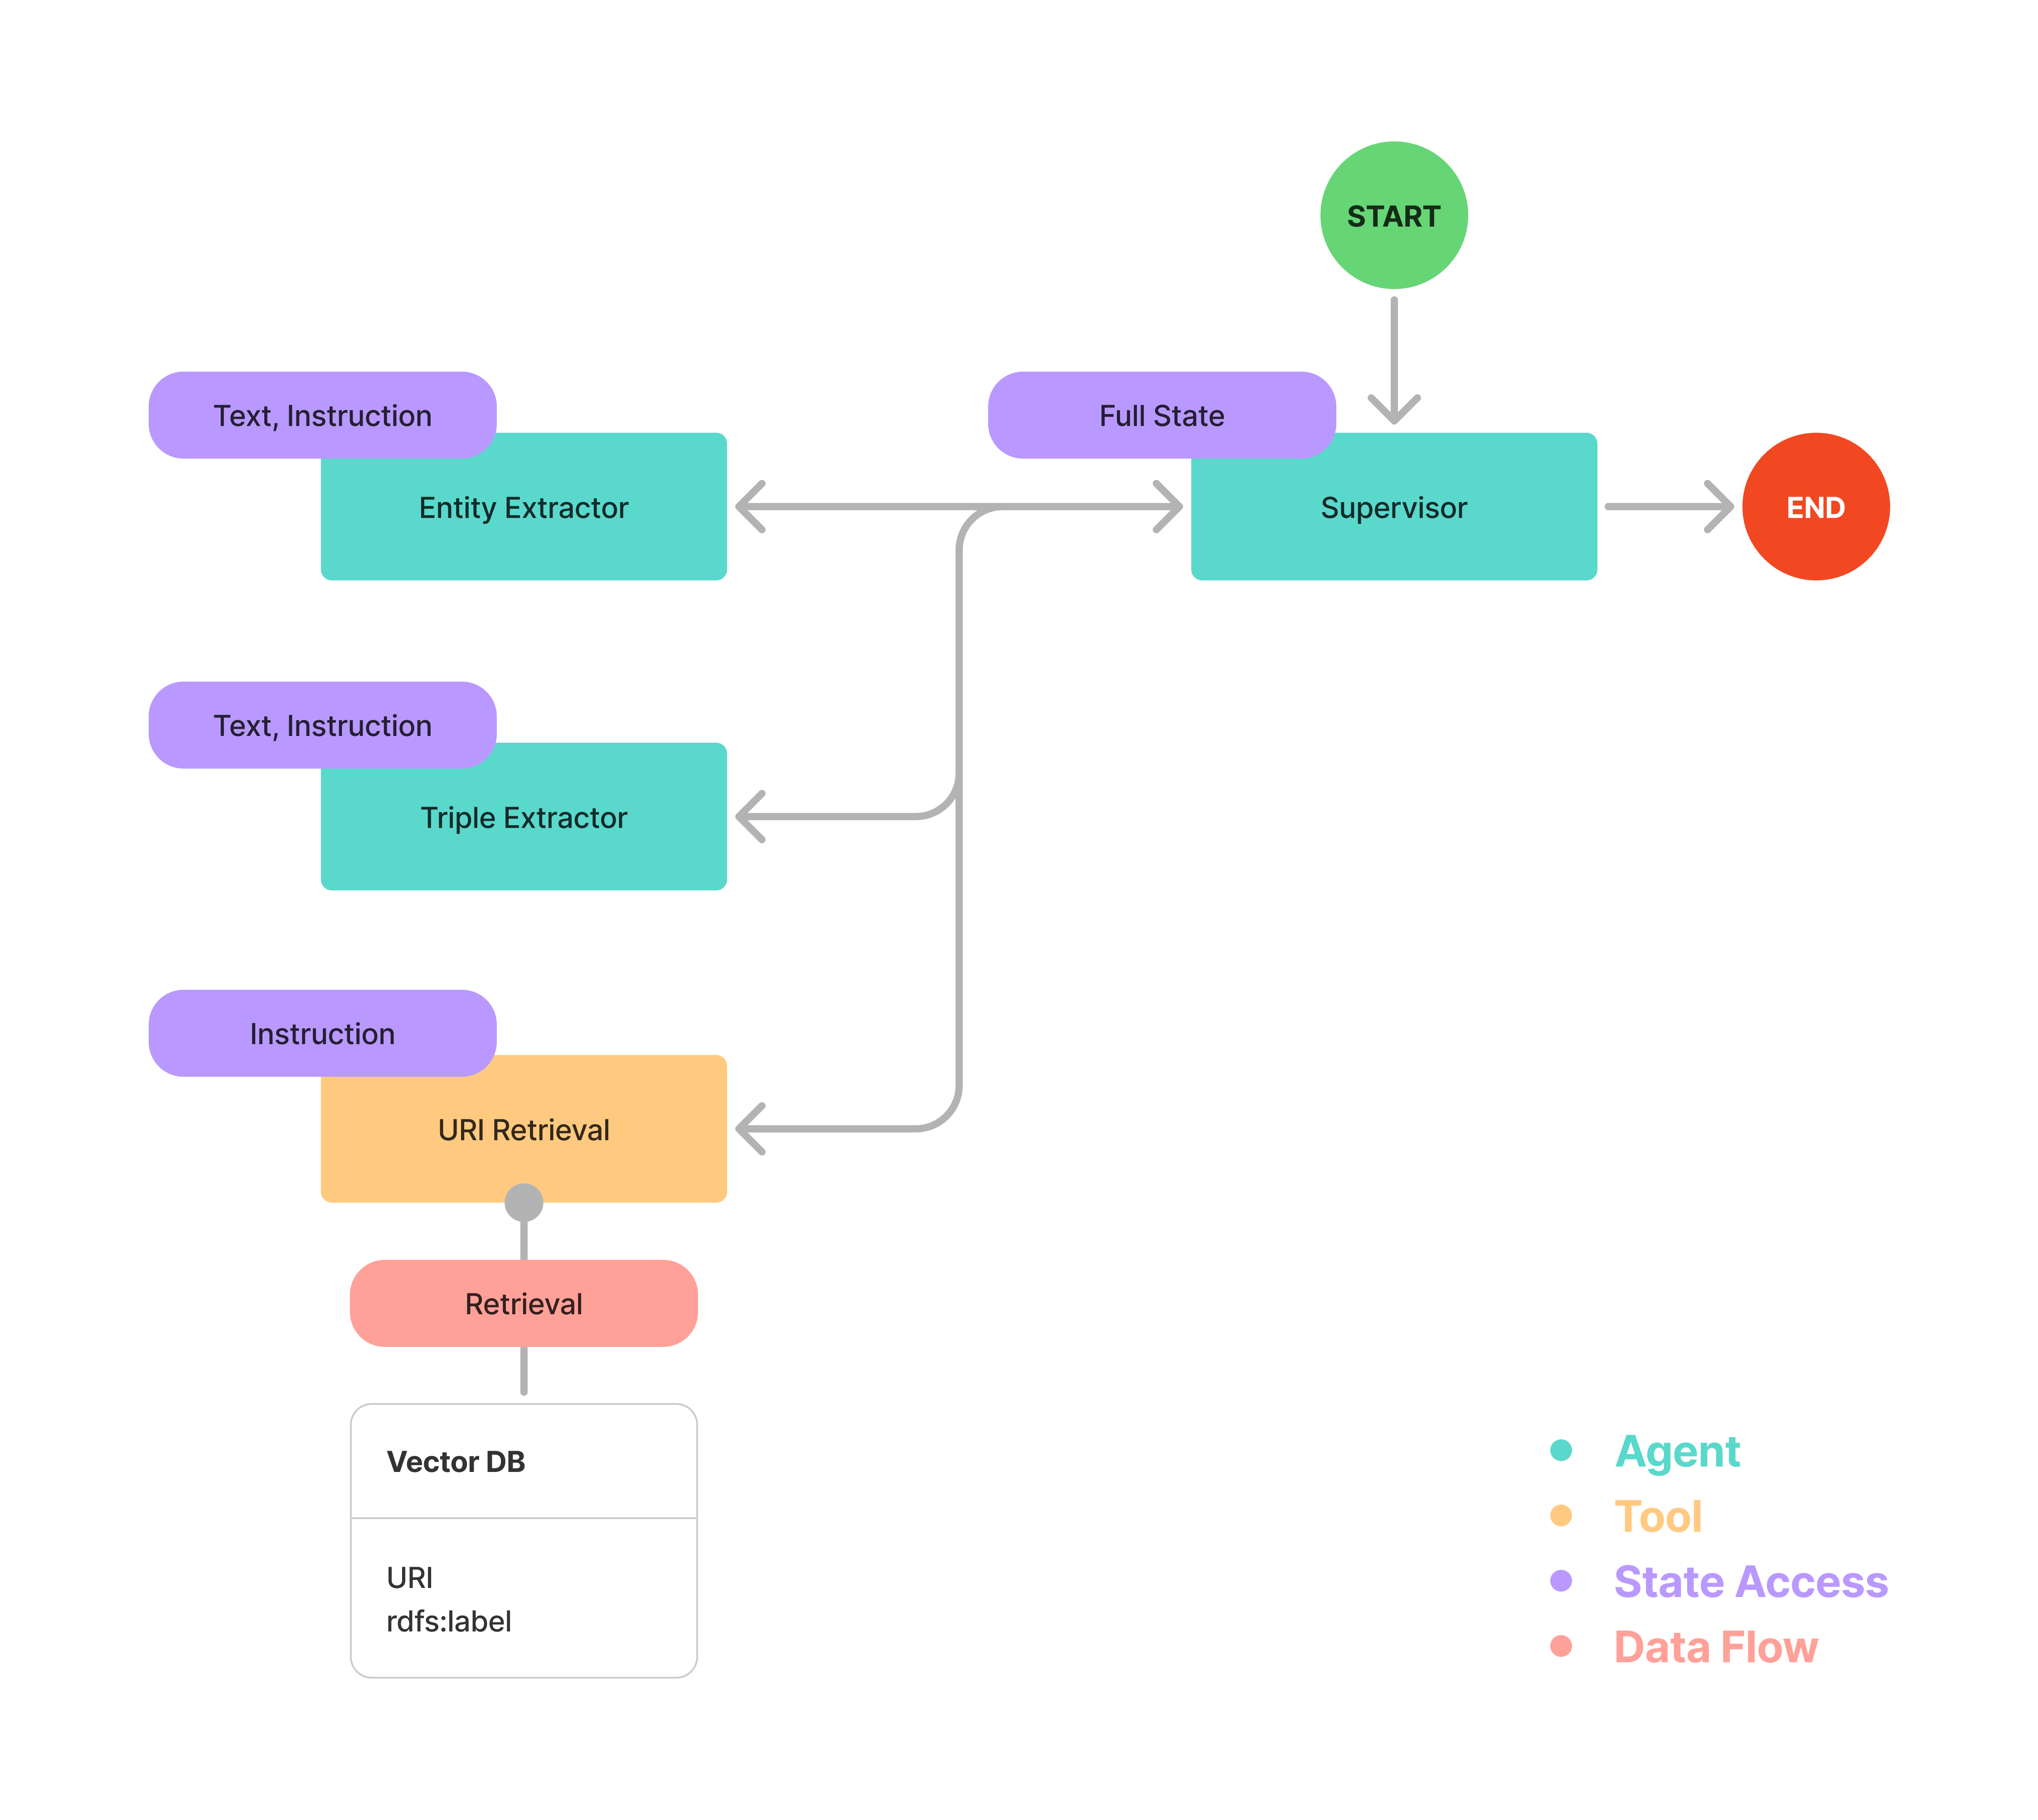
\includegraphics[width=\textwidth]{figures/Baseline Architecture.png}
  \caption{Baseline architecture showing the pipeline approach with specialized agents for each step of the closed information extraction process (self created)}
  \label{fig:baseline_architecture}
\end{figure}

The baseline architecture remarks the first approach used in this work to approach. This architecture follows the pipeline approach of closed information extraction by implementing two specialised agents for extracting and disambiguating the entities and forming triples. The idea follows the multi-agent priciple of splitting down complex tasks like closed information extraction is perceived \cite{Josifoski2021} into simple managable tasks. In addition, the baseline follows the overall principle of the supervisor pattern, by implementing one agent that defines the flow and communication between the agents. The URI retrieval tool is already included in this stage, in order to map the free-text triples to URIs. An overview of this architecture can be found in \ref{fig:baseline_architecture}.

The backbone of the baseline architecture remains the state. The state is build up of the fields text, messages and instruction. The text is part of each state and keeps the text that is being processed by the agent. The messages field is an array of messages send. Therefore, especially the supervisor agent gets access to the message history to prevent looping and enable targeted reasoning. The instruction can be filled with variable that should be given as an input to either a tool or other agents.

In a supervisor architecture like in the baseline the orchestration and routing relies solely on the supervisor agent. In this configuration the supervisor agent is the only agent, which has access to the full state. The supervisor is designed to take additionally care of agent results validation and to formate the final result. This means, that the supervisor is in charge to extract the entities and triples using the specialised agents and then evaluate whether those results are valid or if it has to reiterate with the agents to get better results or to get a entity disambiguation. Therefore, the supervisor agent can leverage the instruction field on the state to pass individual prompt instructions to the agents. With triples formed by the triple extractor, the supervisor agent then has to formulate search terms, that will be search using the URI retrieval tool. With the output the final task of the supervisor is to formulate a valid turtle output. In order to parse the next agents and the final output, the supervisor agent is using xml tags to delimit the parseable outputs.

The entity and relation extraction agent are related on prompt engineering. Therefore, both agents were initially used with a simple prompt asking for entity, respective relation extraction. Further details on the general prompt engineering approach can be found in \ref{sec:iterative_prompt_engineering}. The idea is that over time both agent can tackle the limited task of entity and triple extraction to a very good extend.

All in all the idea can be lead to a flow where first the entities get extracted and then the the triples get formulated. Then the supervisor should get the corresponding URIs and produce a final turtle output. If this straightforward approach fails, for instance because a URI can not be found as the entity or predicate in the triple is incorrect, the supervisor agent can then loop. This shows that in theory this approach can extend the simple workflow by refinements and limit error propogation.

\subsection{Splitted Supervisor Architecture}
\label{subsec:supervisor}

\begin{figure}[h]
  \centering
  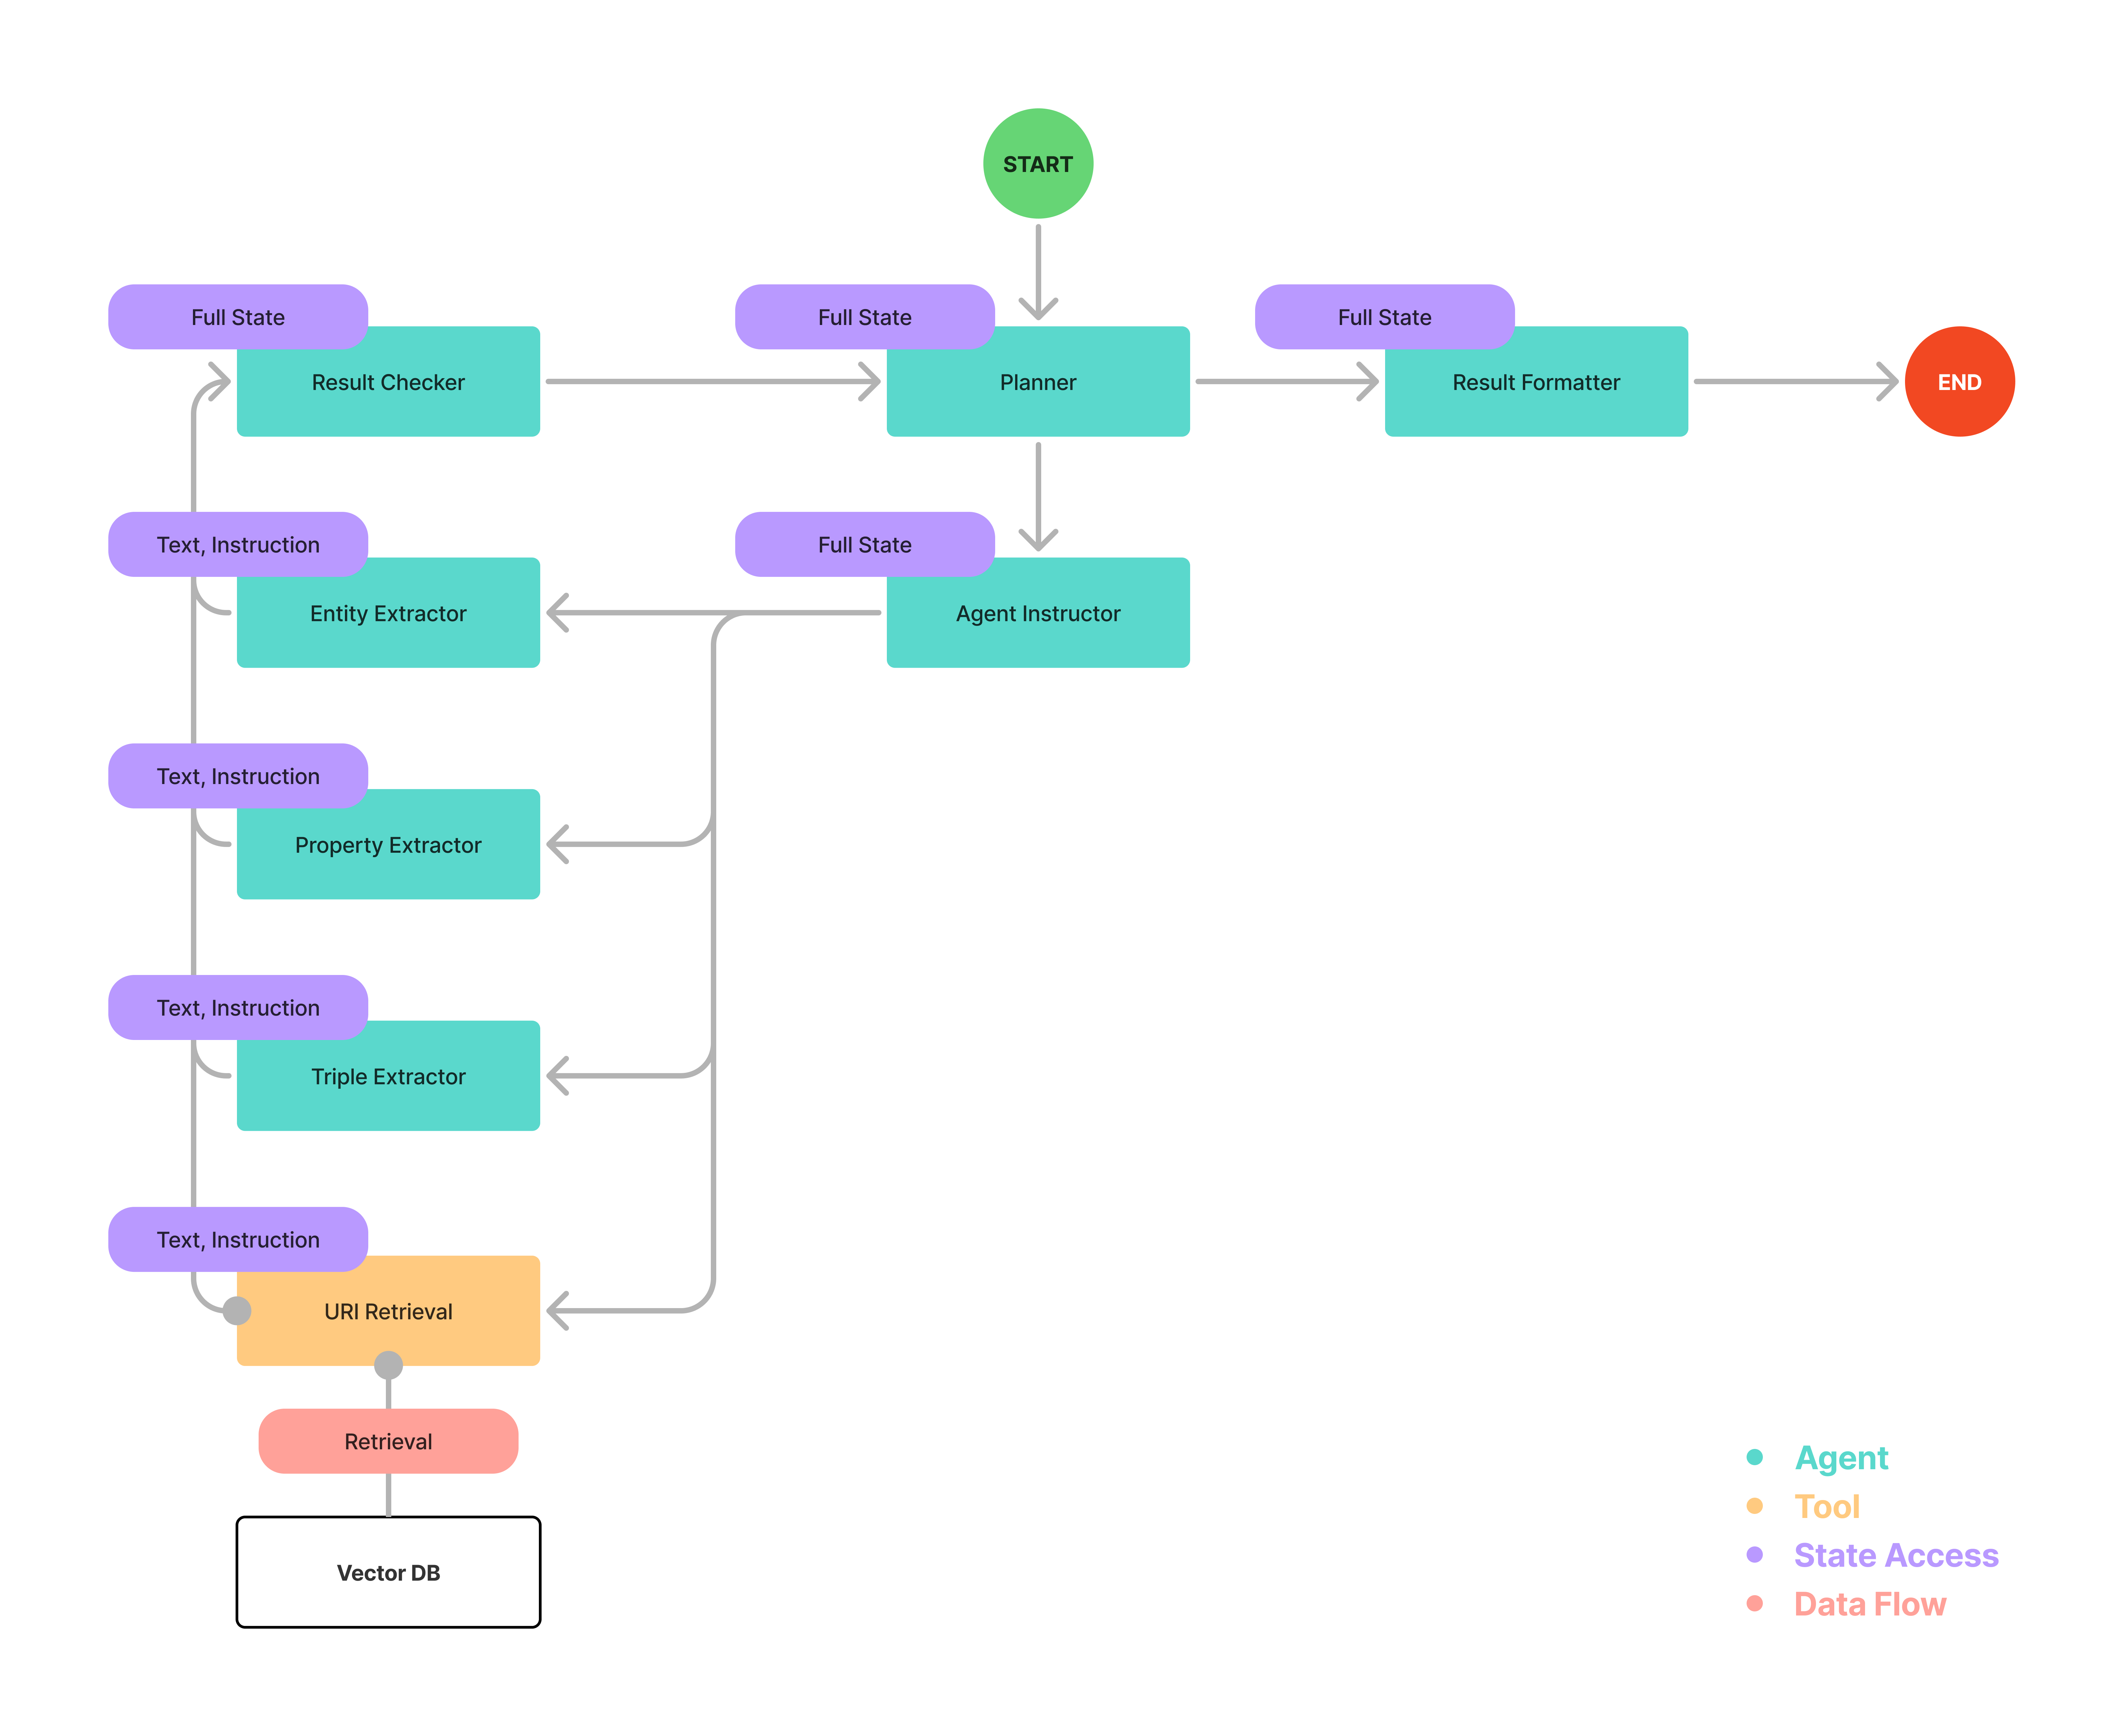
\includegraphics[width=\textwidth]{figures/Splitted Supervisor Architecture.png}
  \caption{Splitted supervisor architecture showing the decomposition of the supervisor agent into specialized sub-agents for better task management (self created)}
  \label{fig:splitted_supervisor_architecture}
\end{figure}

As in the baseline archiecture, the supervisor agents has the task to plan the task, route the task to right agent or tool with the correct instruction and then evaluate the observations from the agent and the URI retrieval tool following up with a refinement of the plan or the output of a turtle string. This task is a rather complex one, especially if the idea remains to iterate over the closed information extraction task. The \ac{SSA} is a step in the iterative agent system design process, to adapt towards \acp{LLM} which are not able to process as many tasks at the same time alongside with an increasing prompt and context size. Therefore, the supervisor agent is split up into a planner, agent instructor, result checker and result formatter agents. In addition the specialised agents (Entity and Triple Extractor) were completed by an property extractor. As the property extractor was added during the iterative process, an exact evaluation of the introduction of this agent can be found in section \ref{subsec:error_message_incorporation}. An overview of the architecture can be found in figure \ref{fig:splitted_supervisor_architecture}.

The state is redefined in the \ac{SSA}, according to provide more overview to the supervision agents (planner, agent instructor and result checker). This means in addition to the text and the instruction, a call trace, a results and a comment field was implemented in the state. The call trace is used by the agent instructor to save which specialised agent or tool was called with which input. The results field is than the counter part where every result of the specialised agents and the URI retrieval are saved. At last, all comments made by the supervision agents are written into the comments field. Doing so, the actual closed information extraction results can be seperated from the overhead communication made by the supervison agents within the state. Furthermore, this can also separate the information within the prompt with idea to give the agents are pre-structured overview of the flow within the multi-agent system.

The planner agent is the central point within the \ac{SSA}. It generates an initial plan and decides whether to how to proceed with the plan or finish the flow by handing over to the result formatter. If the next step of the plan should be executed, the agent instructor refines this action into parseable agent id with the matching instruction. The idea behind is, that the planner can fully concentrate on planning, while the agent instructor can parse ideas into actions. Using a result formatter agent follows this idea and is added up by the complexity of providing a valid turtle output for the selected datasets. In addition, the result formatter is used to put all pieces of information like URI retrievals and extracted triple together.

The result checker agent follows the idea of a real supervisor. It has the task to look onto whether the specialised agents are producing correct results. In addition, the result checker agent should give the planner ideas how to refine the overall processing plan and what information are missing. Therefore, the result checker agent should induce iterating over the closed information extraction task.

The entity extractor and relation extractor agents are designed like in the baseline architecture, but are changed in the point in which field they save their outputs to. The property extractor agent follows the overall plan of the practises designed in section \ref{sec:agent_design}. This means, that the relation extractor is taken apart the task to identify the properties within text. The URI retrieval tool is similar to the one in the baseline archiecture, but as the agents, so does the URI retrieval tool save its output to the results field of the \ac{SSA} state.

Overall the \ac{SSA} is an extensive interpretation of splitting up complex tasks. Therefore, it follows an custom architecture pattern similar to the original supervisor pattern. In addition, the state is changed in order to provide more overview for the added overhead of more agents.

\subsection{Simplified Splitted Supervisor Architecture}
\label{subsec:simplified_splitted_supervisor}
\begin{figure}[h]
  \centering
  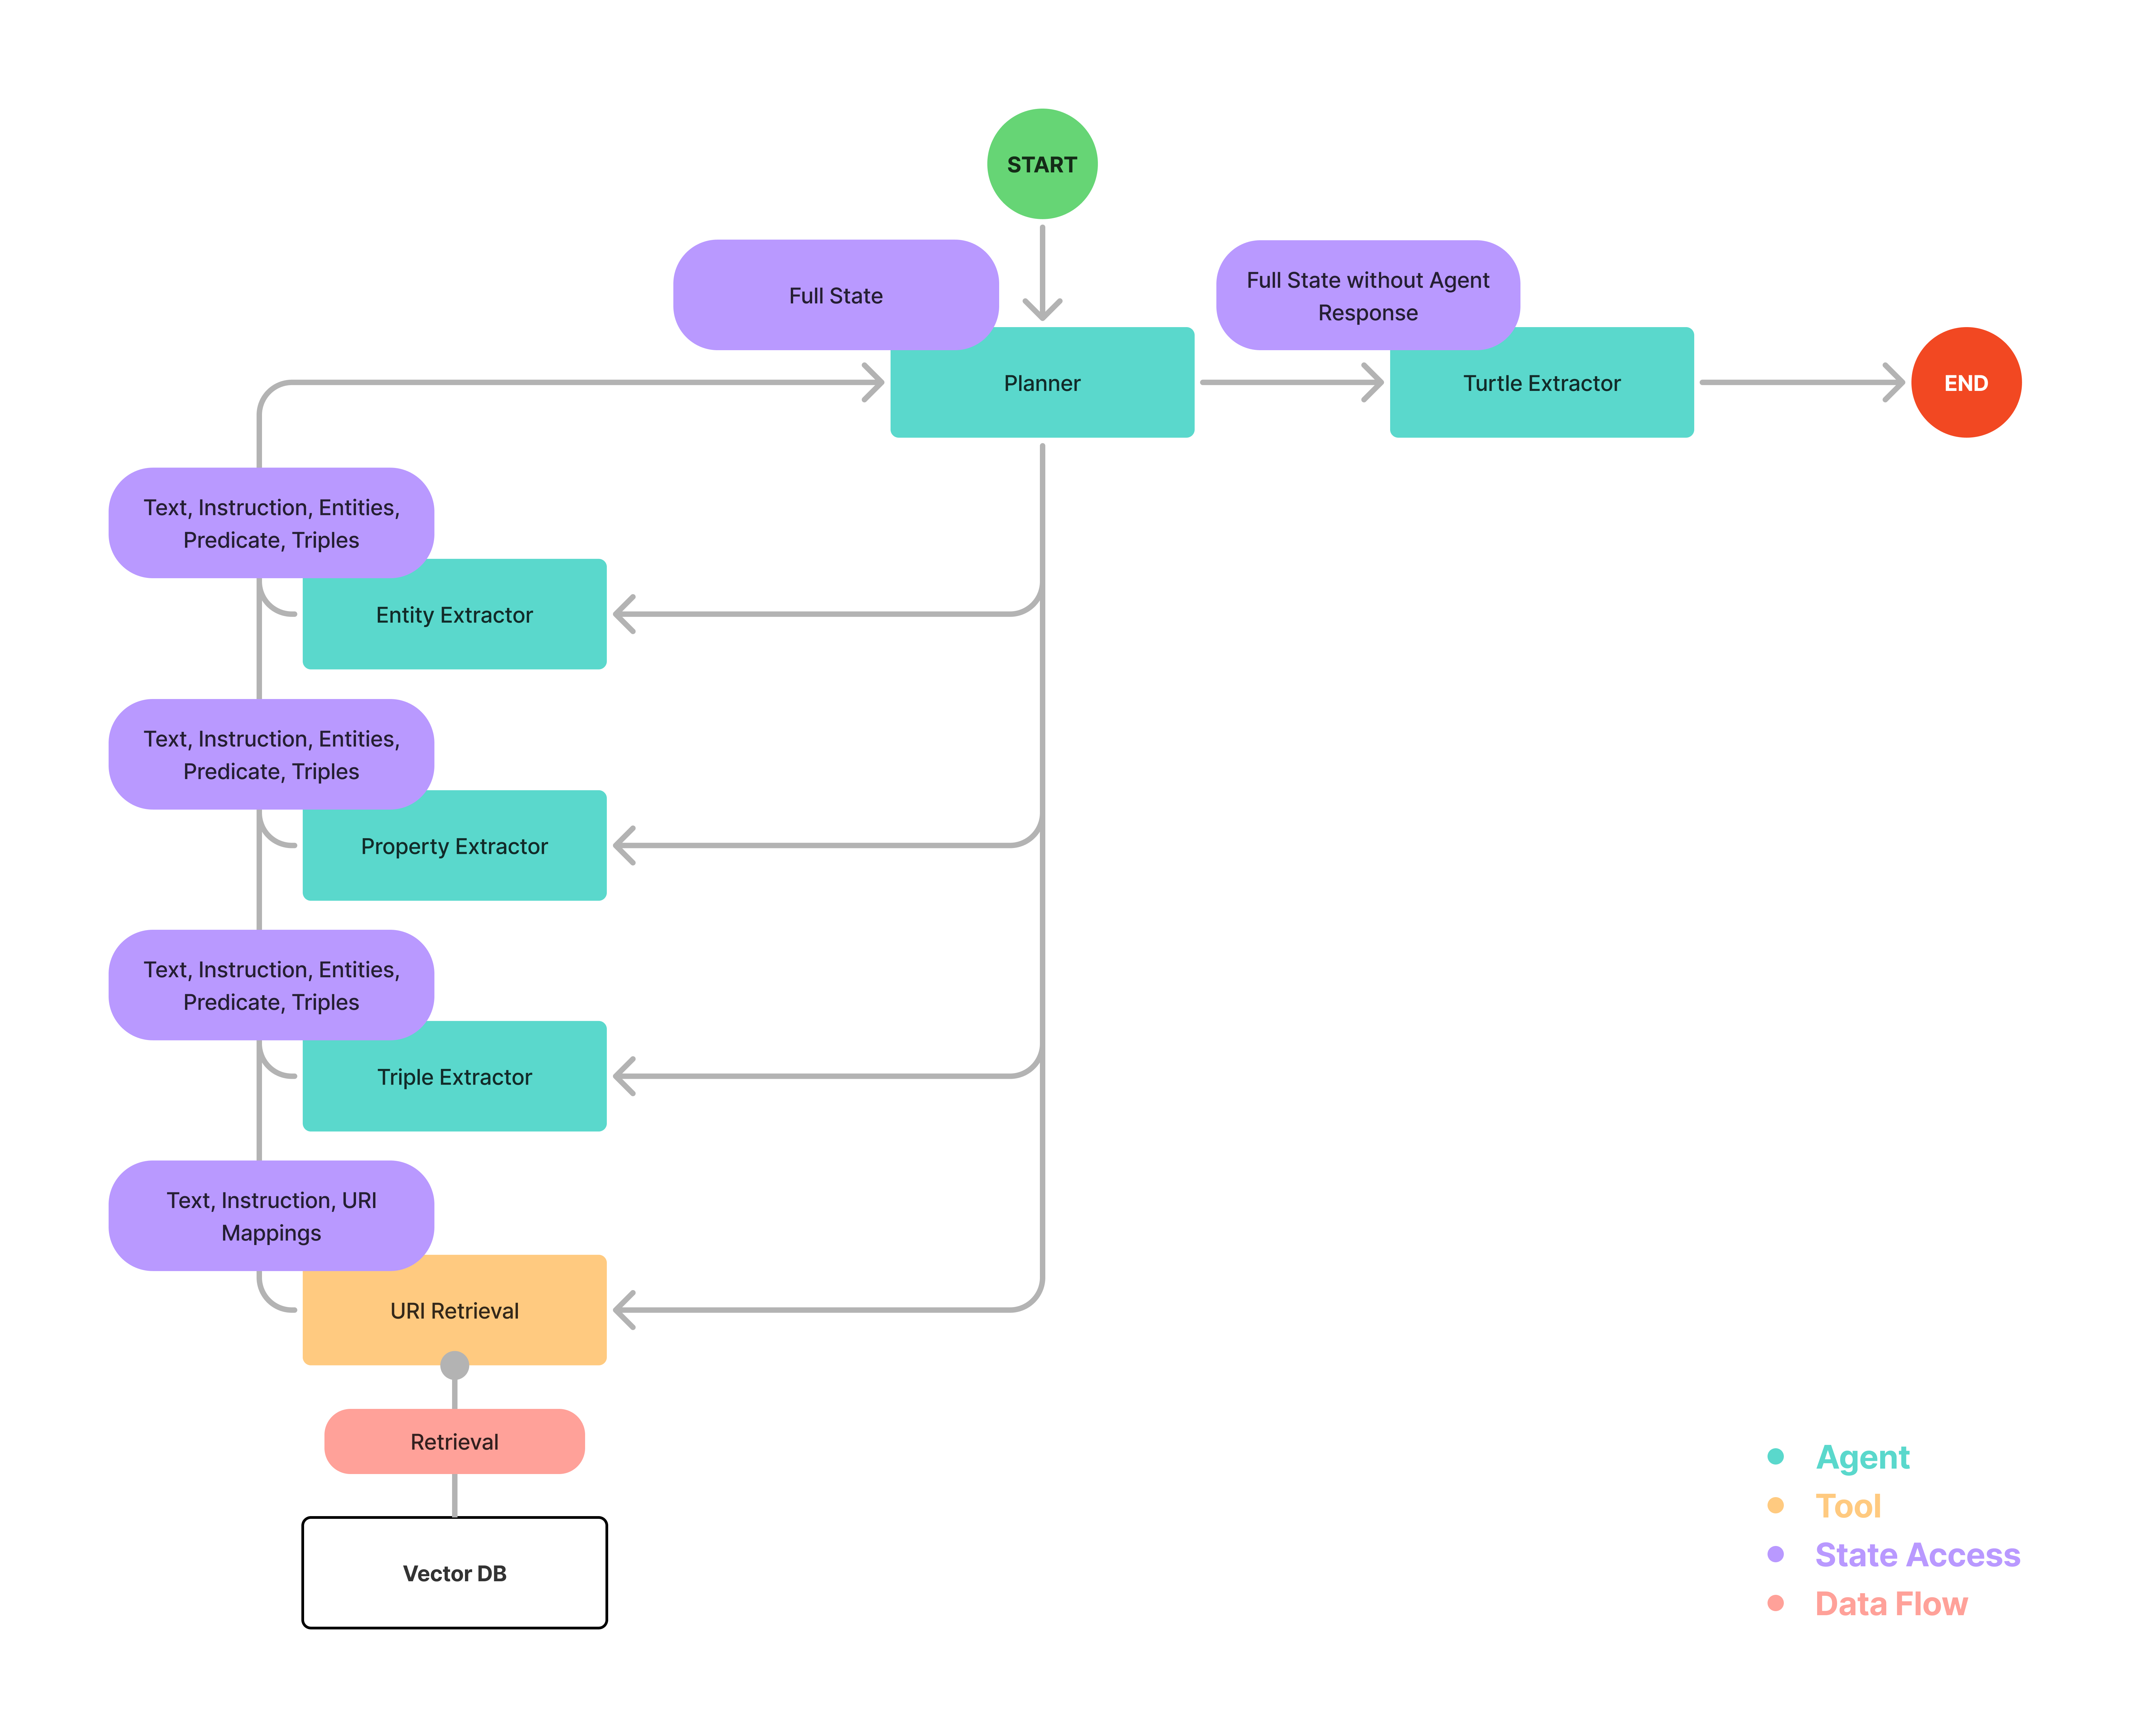
\includegraphics[width=\textwidth]{figures/Simplified Splitted Supervisor Architecture.png}
  \caption{Simplified splitted supervisor architecture showing a streamlined version of the supervisor decomposition with optimized agent interactions (self created)}
  \label{fig:simplified_splitted_supervisor_architecture}
\end{figure}

The \ac{SSSA} is following the general idea of the \ac{SSA}, but uses a simplified supervisor splitting. Based on the assumption that a single supervisor can handle all supervison task, but struggles with putting together the triples and URIs to valid turtle strings and using an unstructured state as context. Therefore, all specialised agents remain the same as in the \ac{SSA} and result checker and agent instructor are merged into the planner agent similar to the supervisor agent of the baseline archiecture. Additionally, the mapping of results of the agents is adapted to an updated and more structured state. An overview of the the architecture can be found in figure \ref{fig:simplified_splitted_supervisor_architecture}.

A core change in comparison to the \ac{SSA} is the overall structure of the state. In order to sleeken the state, the \ac{SSSA} state just keeps the core of the result of the specialised agents. This means, that the state has now field for entities, properties, triples and URI mapping instead of a single results field. Those fields will be filled by the specialised agents and the URI retrieval.

As this state change deletes the full output of specialised agents and of the URI retrieval, a field agent response is added that exposes the full output of the speicalised agent, but also tools to the planner to detect, if the agent are processing the tasks given correct. In order to prevent looping, the message field in the state remains the same, but is now the output history of the planner agent.

Overall the \ac{SSSA} is designed for less resource consumption and more efficient context use. The architecture is mainly designed towards context limits, that can apply, while keeping the idea of iterating over the process. In addition, it is another approach to split up the supervisor agent and therefore it remains an architecture following the custom multi-agent system pattern.


\subsection{ReAct Architecture}
\label{subsec:react}

\begin{figure}[h]
  \centering
  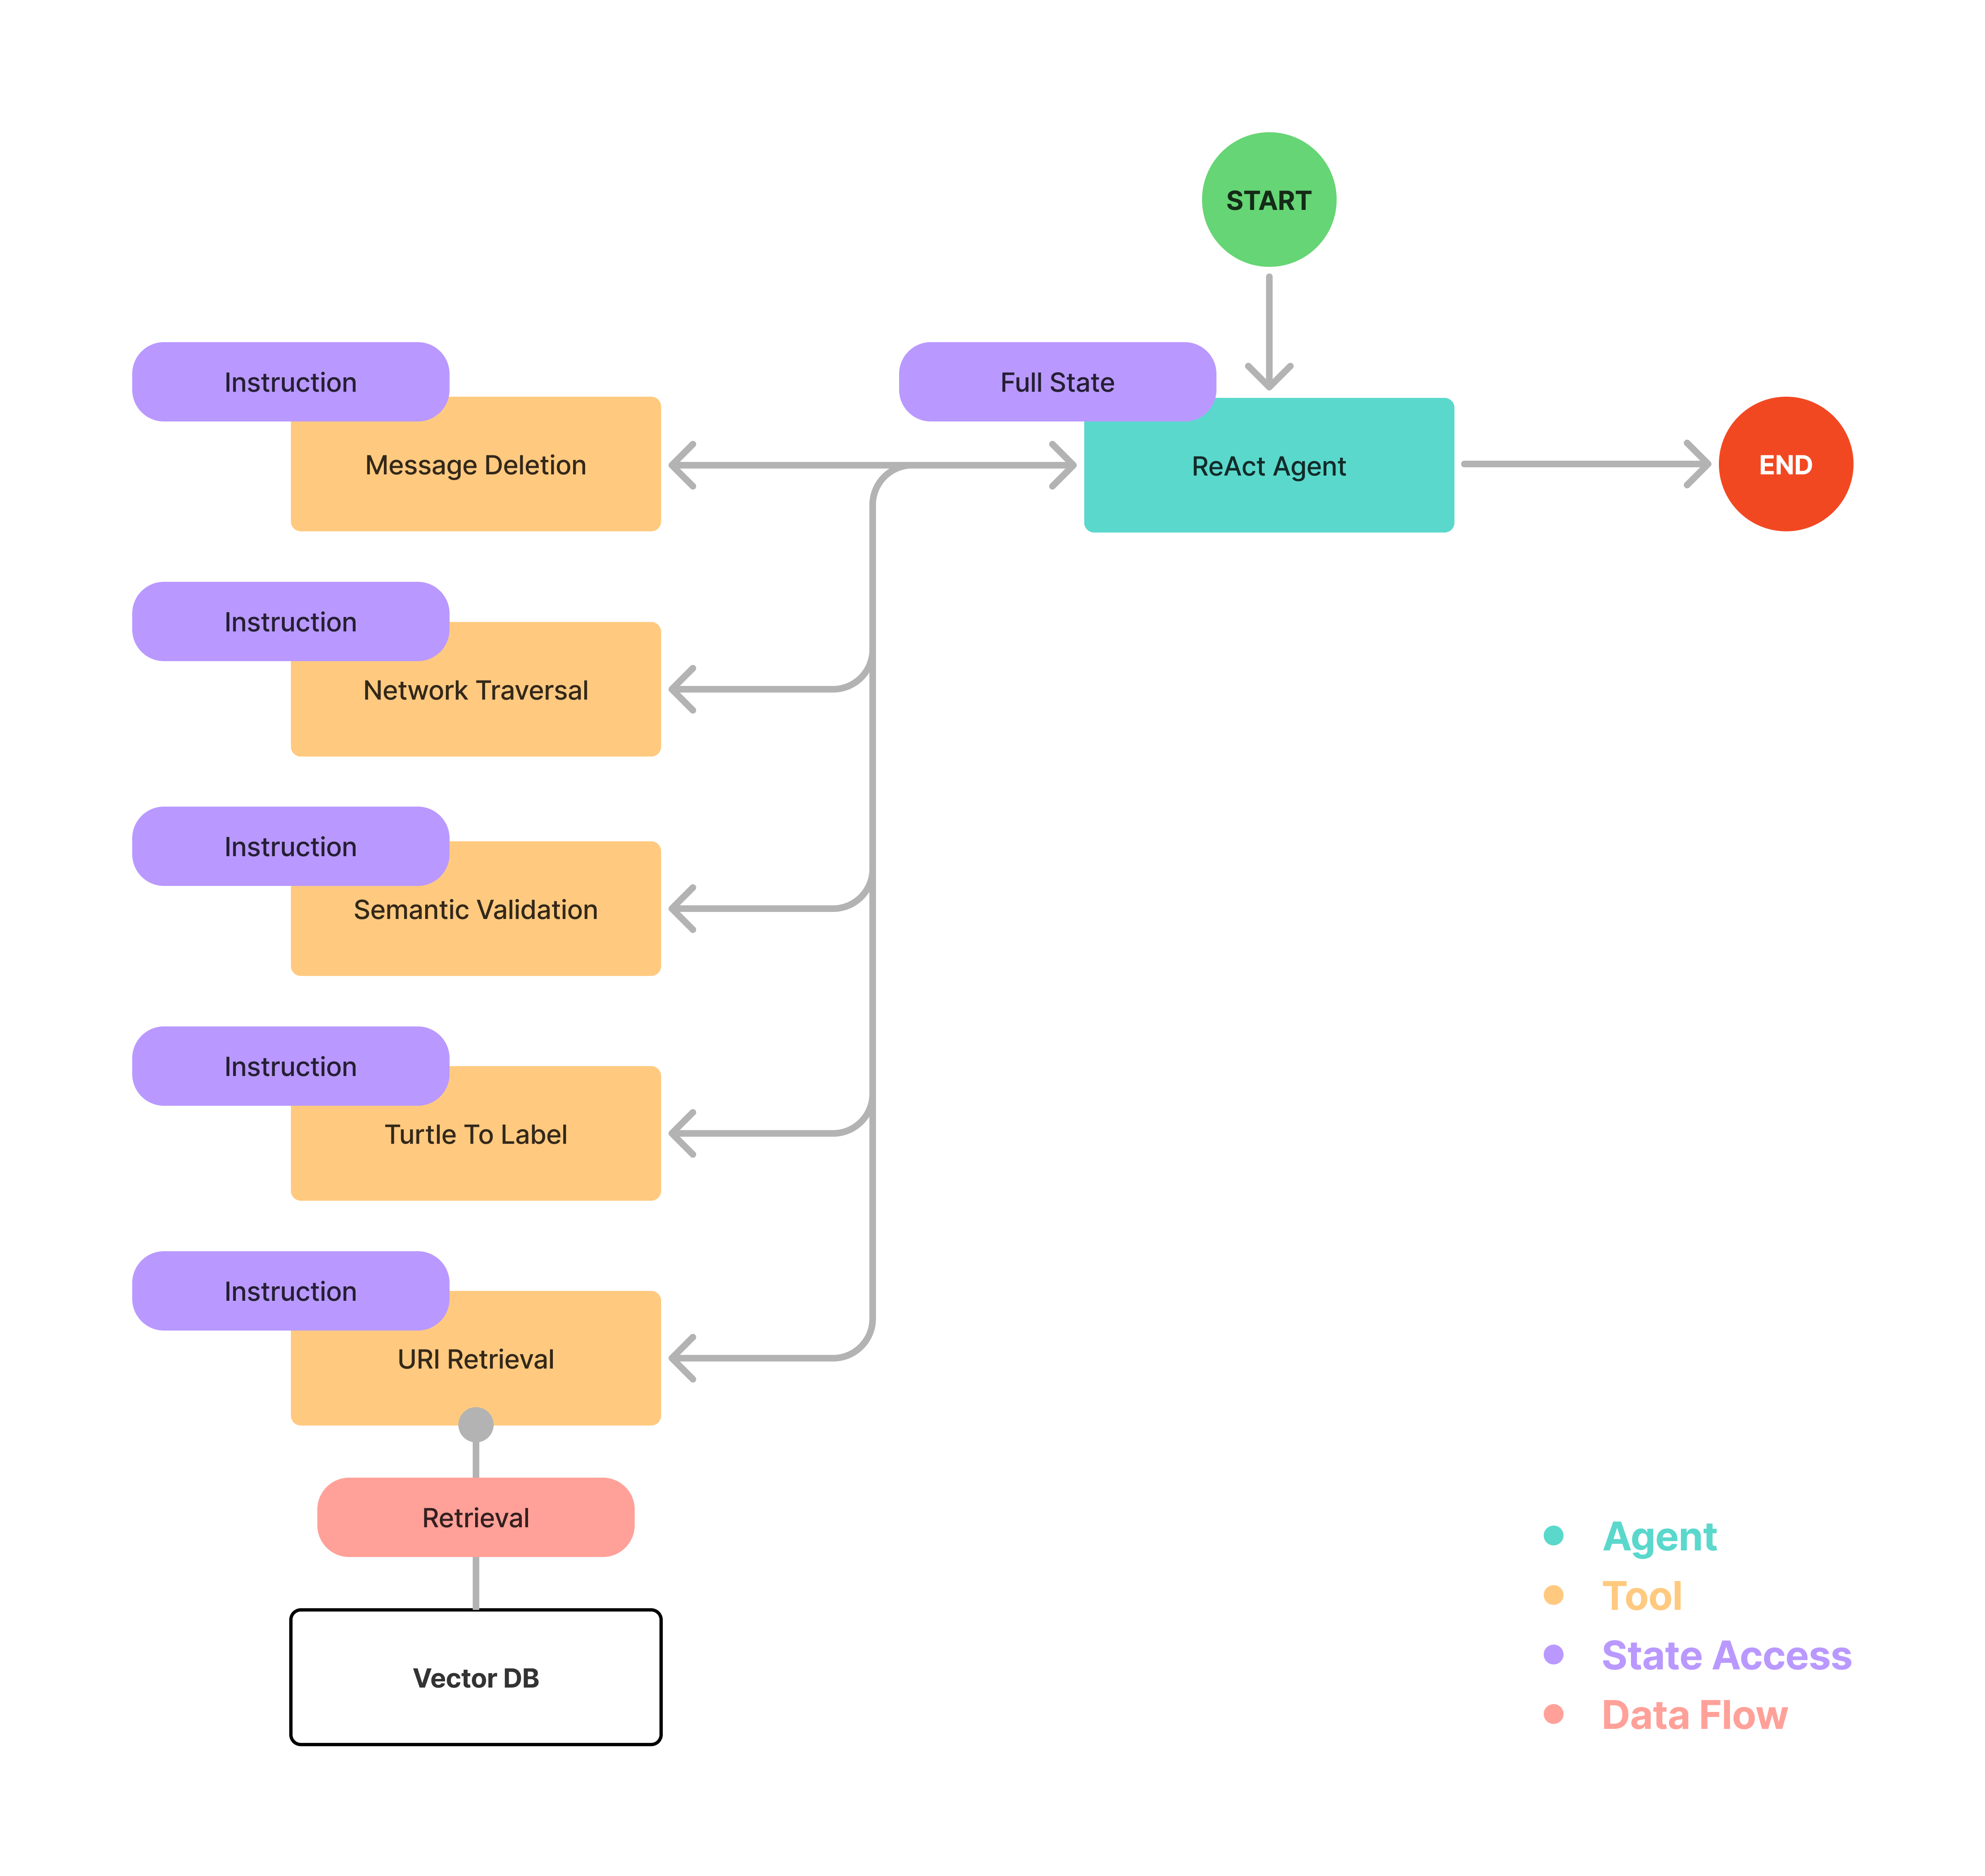
\includegraphics[width=\textwidth]{figures/ReAct Architecture.png}
  \caption{ReAct architecture showing the single-agent approach with reasoning and action capabilities for closed information extraction (self created)}
  \label{fig:react_architecture}
\end{figure}

All previously shown solution rely on multi-agent system, as of the assumption of high complexity wihtin the task of closed information extraction. The ReAct architecture is targetting an opposite direction. The idea is to show, how capable a single-agent system with reasoning capabilities can be, as simplicity often showed empirical success within the work. In addition, the ReAct architecture can solely concentrate of incorporating with tools other than incorporating with agents which increases the possiblity for failures. Like already state in section \ref{sec:related_approaches} a joint-optimisation has the advantage of a single-optimisation point with no error propogation. The ReAct architecture follows this joint-optimisation. Another conceptual advantage is that the agent calls are reduced, which results in lower cost and lower inference latency.

The state is also made simpler than in the \ac{SSA} and \ac{SSSA}. As the agent calls get reduces, so does the context. Therefore, the baseline state shown in section \ref{subsec:baseline} is used as well. The tools are writing their outputs into the messages field.

As the agent is limited in its availablity to handle the task to the full extend, it is initially given URI retrieval tool. As the ReAct architecture showed a good optimisation capability further tools were developed for it. First, there were tools to incorporate and communicate with the knowledge graph, namely the network traversal, semantic validation and turtle to label tool. Second, to give the agent the ability to manage the context, a message deletion tool was implemented. A overview of the tools used in the ReAct architecture can be found in figure \ref{fig:react_architecture}. As outlined, there were multiple iterative steps within the development of this architecture. All of them will be review in section \ref{sec:evaluation_configurations}.

The ReAct architecture is not a multi-agent system, but it remains one step to contrast highly complex systems in order to develop an understanding of the \ac{LLM} used for the closed information extraction. As of its cost efficiency it remains a good point to start to develop more tools and to test which of them are providing a leap over the previous configuration. Therefore, the ReAct architecture is a logical iterative step to a target architecture.

\subsection{Network Architecture}
\label{subsec:network}

\begin{figure}[h]
  \centering
  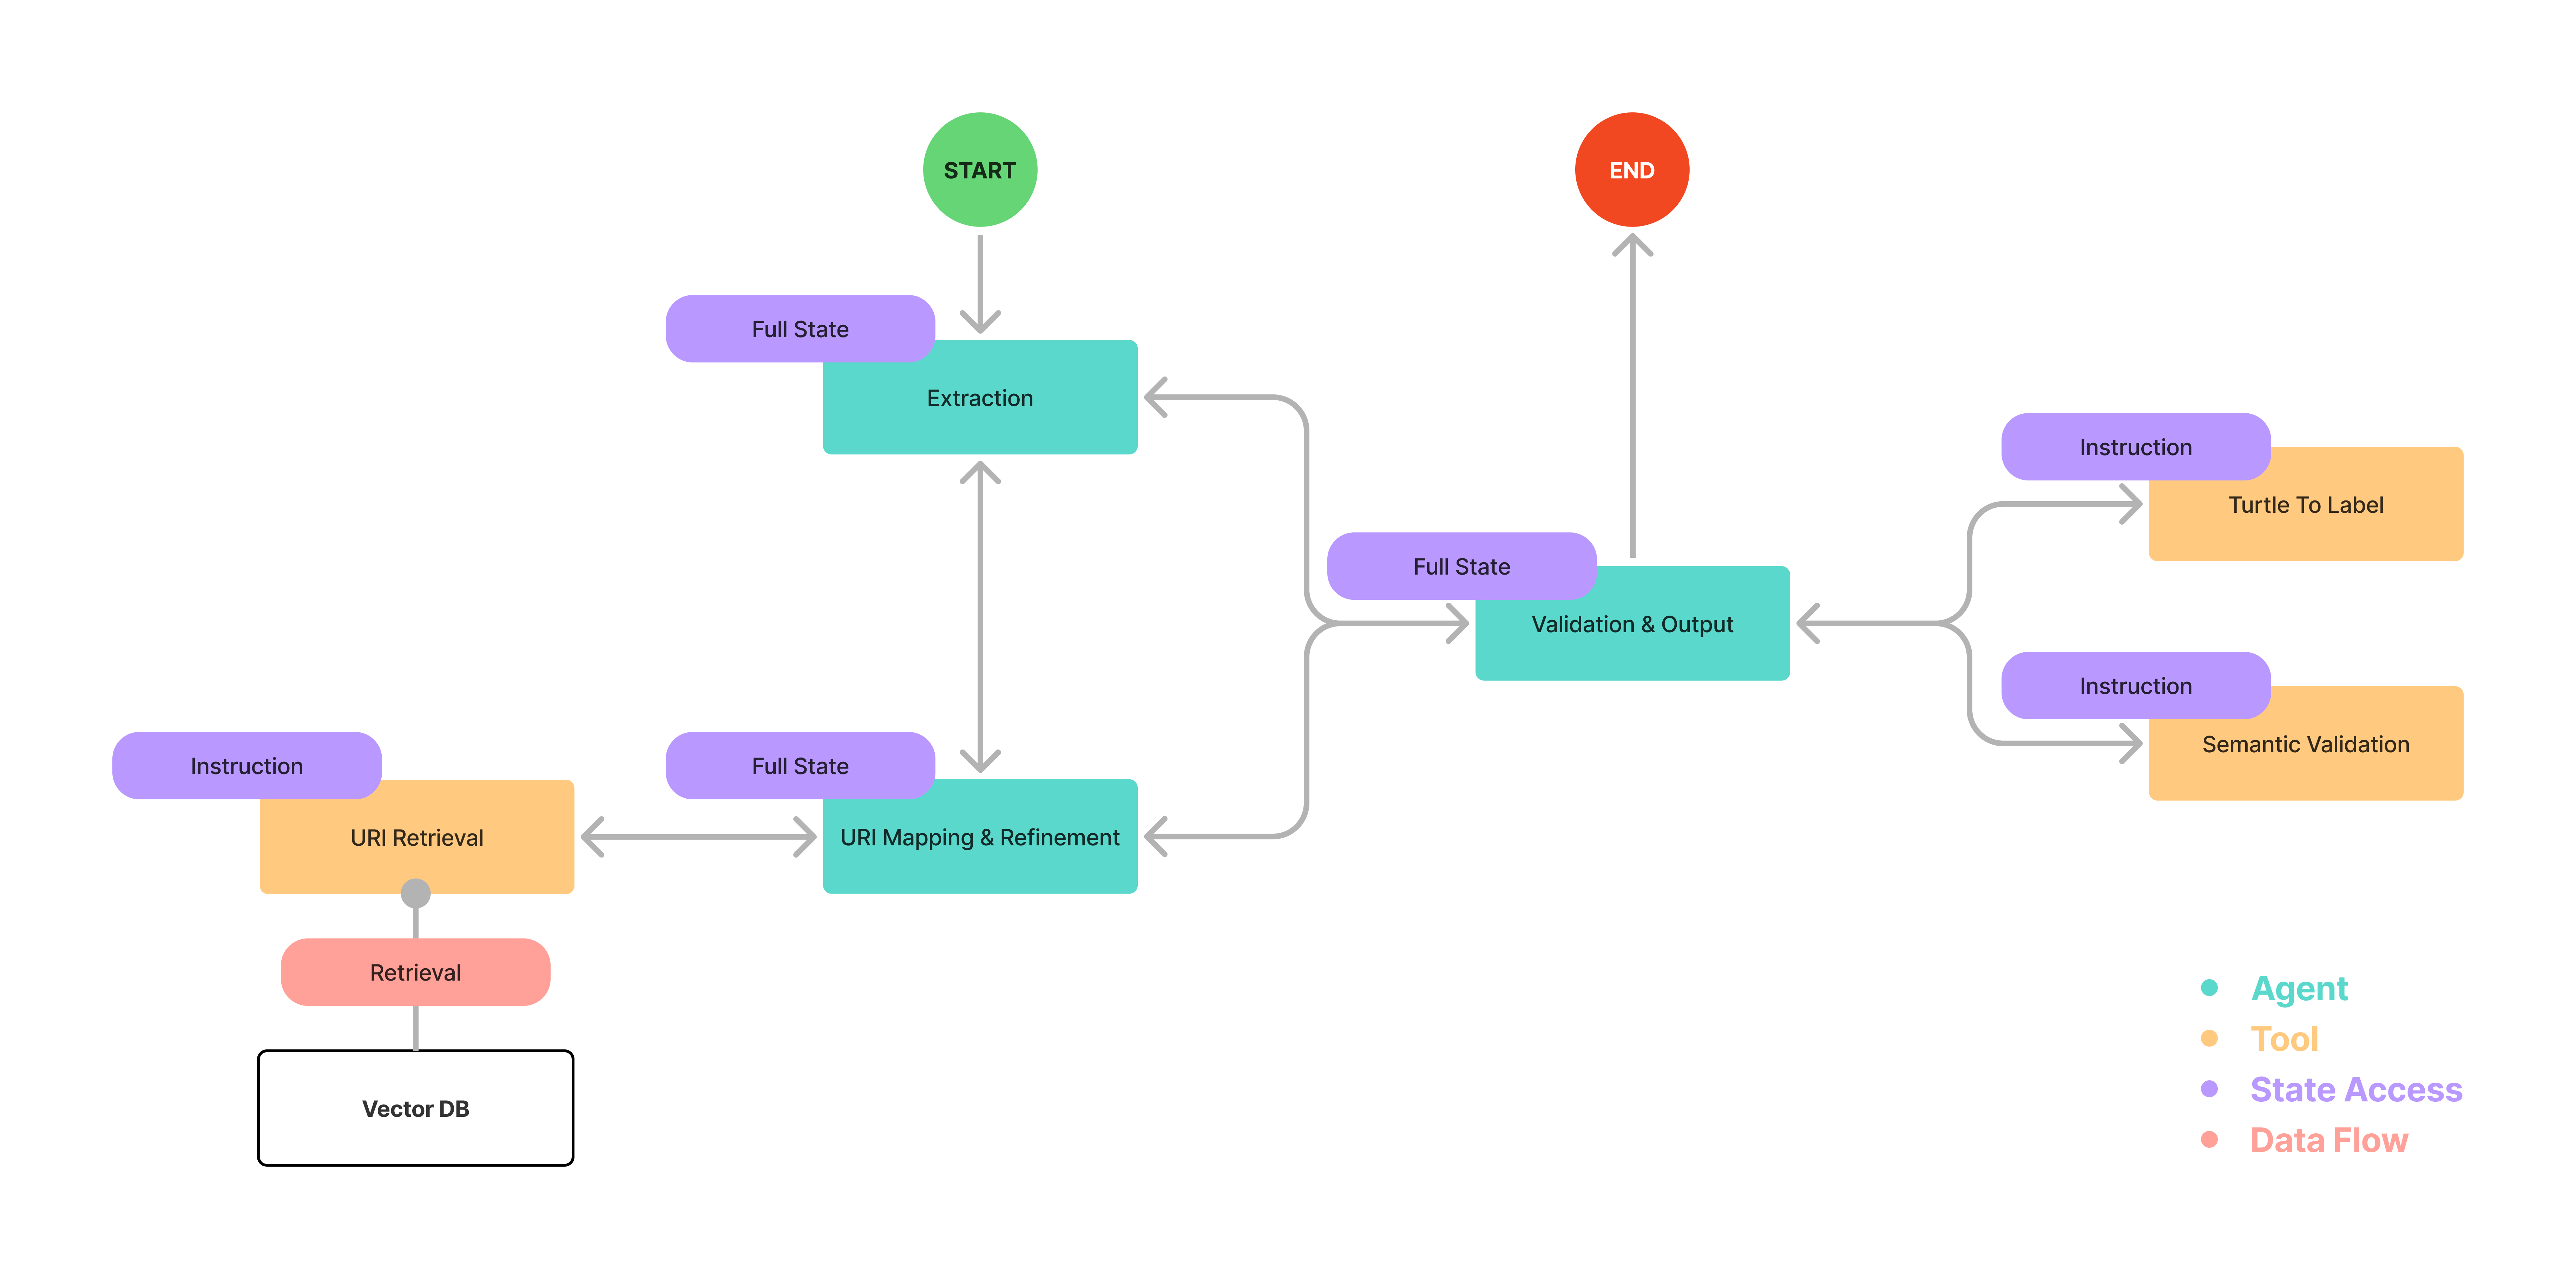
\includegraphics[width=\textwidth]{figures/Network Architecture.png}
  \caption{Network architecture showing the fully connected multi-agent system with dynamic routing and reasoning capabilities (self created)}
  \label{fig:network_architecture}
\end{figure}

The network architecture following the idea of the network pattern outline in section \ref{sec:multi_agent_systems} is the result of the experience made with all previous architectures but also with all different configurations of tools and states. Therefore, the idea is to leverage the reasoning and validation capabilities build up within the \ac{SSA} and \ac{SSSA} and combine it with a direct triple extraction approach like shown in the ReAct architecture. In addition, the network architecture spreads the decisions about the flow on all used agents. The resulting architecture figure can be found in figure \ref{fig:network_architecture}.

The state of the network architecture is a extension of the idea within the state of the \ac{SSSA}. The idea is again to save intermediate results in a context efficient way. Therefore, the fields triples and uri mapping are again part of the state. The URI mapping contains in this architecture the label of the entity or predicate alongside with the URI and the label and description stored in Wikidata.

In addition, a call trace is introduced again to prevent looping and enable logical reasoning. To provide a good overview, the last agent or tool call is stored alongside the response in the fields \texttt{last\_call} and \texttt{last\_response}. In addition, the \texttt{agent\_instruction} field is introduced to persist the instruction given to an agent by a previous agent, while not being dropped within a tool call. The input to any tool is persisted in a \texttt{tool\_call} field. A \texttt{message} field is also introduced, but unlike in other architectures, in the network architecture it is used to output the final result, which is based on interoperability considerations.

This architecture is also thought to minimize context length by not having any field in the state that builds up content increasingly except for the call trace. Therefore, the agents have to decide on the next steps utilising the previous call trace and the current results. This increases the reliability requirements for each agent and could potentially be a point where heavy prompt engineering must be used.

Agent-wise the network architecture uses three agents, which all have access to the full-state, while the tools are using solely the tool input given by the agents. This is done, because each agent needs to have the full overview to take better decisions on the overall agentic flow. All inquiries start at the extractor agent, which follows the idea of the main agent in the ReAct architecture, but splits the URI mapping, triple validation and turtle output part from it. The extractor agent has write access to the triples as the only agent in the architecture.

The URI mapping is done by the URI mapping and refinement agent. It is thought to be the central place where the URI mapping gets generated or changed on request. Therefore, it is the only agent with write access to the URI mapping. The agent is also bound to the triples extracted by the extractor agent. Tool-wise the URI mapping and refinement agent has access to the URI retrieval tool.

The validation and output agent has the task to prevent halucination of the agents and also validate triples based on semantic features which are used in the knowledge graph. Therefore, the agent is asked in its prompt to do a semantic validation followed by a turtle to label conversion to check the results. Both steps are based on tools that are connected to the validation and output agent. The validation and output agent is also the point to refine and polish the results, if they fall through a validation. Then the agent is able to call either the extractor or the URI mapping and refinement agent again, in regards where it assumes the error can be solved.

The network architecture is a results of the experience gathered throughout prior work. Therefore, it already misses out on unpromising tools or uses a highly tweaked state. In the end, the network architecture remains a multi-agent system in its core idea, while keeping the overhead and context length minimal.

\section{Agent Tools}
\label{sec:agent_tools}

The agents in the various architectures are the core of the solution to the closed information extraction. As \acp{LLM} are limited in their knowledge and also can show hallucination like shown in section \ref{sec:language_models}, the tools are necessary to limit both caveats and on the other side improve the performance. Therefore, two general types of tools are used in this work. First, the knowledge graph incorporation tools, which are URI retrieval (section \ref{subsec:uri_retrieval}), network traversal (section \ref{subsec:network_traversal}), semantic validation (section \ref{subsec:semantic_validation}) and turtle to label (section \ref{subsec:turtle_to_label}). Second, the tools to orchestrate the agent system. In this work, just the message deletion tool (section \ref{subsec:message_deletion}) is proposed.

\subsection{URI Retrieval}
\label{subsec:uri_retrieval}

The URI retrieval tools remains a central tool in solving a closed information extraction task. Various \ac{LLM}-based agents can achieve a extraction of free-form triples, but the challenge of closed information extraction remains in the correct mapping to the underlying knowledge graph. Therefore, this URI mapping ability is given to the agents by the URI retrieval tool, which is able to incorporate with the knowledge graph.

The general idea of the URI retrieval tool is to get individual search terms of the agent and then search for it using embeddings and their cosine similarity. The instructions are ideated to be variied throught the iterations. Therefore, the agents can re-search for entities or properties that were not found by using the simple free-form text.

In order to provide embeddings of the underlying knowledge graph it is needed to pipeline the generation of a search index. The pipeline is executed against the Wikidata knowledge graph, as this is the only knowledge graph used in the benchmarks evaluated in this work. In the final implementation three search indices exist. Those indexes keep embeddings for either the \texttt{rdfs:label} or \texttt{rdfs:description} of an entity in Wikidata. The third search index is saving triple examples for the use of a specific properties out of Wikidata. The idea is, that the sentence embeddings can embed semantic features of subject and object, which later can be retrieved by the agents.

The pipeline works in three steps. The first step is loading a dataset split like the test-split on synthIE with a limited number of documents to be loaded. The second step is to get the label and description for all entities and properties inside the data loaded. In addition, the example triples for the properties will be retrieved for the properties if existing in Wikidata. In a third step all parts will be embedded and saved into the corresponding search index. In order to provide label and description as well as a distinction between entity and property, those data will be stored as metadata in the search index.

In order to provide access to the various collections, the URI retrieval tool required search modes in the instructions. This means, that the agent can decide whether it wants to similarity search its search term agains all labels, description or examples of an entity or property. In addition, as the URI retrieval tool can access the type of a stored point in the search index, the instruction does get another filter mode, where the agent can decide if it searchs solely for entities or properties. In the last implementation a mixture of search and filter modes is used. In this case the agent can decide whether it search for entities or properties by its label or it searches for properties by an sentence. The trajectory of the work resulting in this limitation can be found in section \ref{sec:evaluation_configurations}.

The URI retrieval tool itself parses the instruction and the search mode, respective filter mode per search term. Afterwards, it execute a cosine similarity search using the embedding of the search term on the selected search index. The search result includes the most similar results with their rdfs:label, rdfs:description and their URI.

In cases with agent architectures that are prone to have a problem with context bloating, this can show problem when many search terms are used. In order to take care of this, the URI retrieval tool gets an additional \ac{LLM} call, that should evaluate if one search result matches by looking on the given output. Afterwards it returns a simplified URI mapping, with a reason why a mapping has been choosen, but without the full information about other results and information about descriptions of the search results. This is especially used in the baseline architecture, the \ac{SSA} and the \ac{SSSA}.

All in all the URI retrieval tool is ideated to give the agent the maximum flexibility in searching matching results. Therefore, it indexes the relevant parts of Wikidata within a search index, which later can be retrieved by the agents, which in general follows a retrieval augmented generation idea. As the URI retrieval tool is the tool where much accuracy can get lost, it is the most changed tool throughout the work, which can be seen in section \ref{sec:evaluation_configurations}.

\subsection{Network Traversal}
\label{subsec:network_traversal}

The network traversal tool is the next step in knowledge graph incorporation. The idea targets the problem of agents choosing super or sub-properties of a searched property. This problem could arise especially, when the sentence does not include the exact label of the searched property. The network traversal tool should give the agents the ability to get insights in the knowledge graph property hierarchy by executing SPARQL queries on the knowledge graph.

In Wikidata the property \textit{subproperty of} is used to show this relation. The SPARQL query then searches for all direct super- and subproperties of a targeted property. In addition the SPARQL query is enhanced by a label query, searching for the corresponding labels of the found properties. Then the network traversal tool creates an output consisting of the label and example triple, if one exists for the found property.

Some properties can have a vast amount of super- and subproperties. This can lead to a unsorted output, where \acp{LLM} can struggle selecting the relevant property from the output. That is why, in later implementations the network traversal tool checked the possible properties for property constraints. In Wikidata there are subject and object type constraints, that can be accessed behind qualifiers.

Qualifiers in wikidata is a triple consisting of a predicate and an attribute \cite{Wikidata2025}. For the subject and object type constraint, the property named property type constraint is used. This property has either the property subject type constraint or the property value type constraint for the object. The attribute is than the actual URI of the type that the original property is constrained to.

Using this knowledge the SPARQL query used in the network traversal tool could output whether a properties subject and object type constrained have been matched or not. This is also done by using one level of superclasses above the type of the particular subject or object in the corresponding triple. This is limited due to the exploration about infinite looping by not restricting, when accessing Wikidata directly like done in this implementation.

Utilising the output of the network traversal tool, the agents are enabled to detect to narrow or to wide property extractions. This gives a better insight in knowledge incorporation for the agents and can make the results more correct. Nevertheless, the network traversal tool can produce a high amount of results, which can be adding overhead to the agents, as they have to decide if any of the resulting properties is fitting better into the extracted triple, while resisting properties that might match the property constraints more, but could be either to narrow or to wide.

\subsection{Semantic Validation}
\label{subsec:semantic_validation}

As \acp{LLM} can show hallucination and additionally do not have the build-in the ability to double check their results, the semantic validation was ideated as solution. The overall idea is like in the network traversal tool, to check for type restrictions on each property of each resulting triple. The semantic validation tool uses a pre-filtered Wikidata class hierarchy, which is loop-free and therefore enables to search across the full hierarchy.

The semantic validation tool gets as input a ready turtle string, which gets checked and afterwards splitted into triples and per triple in subject, property and object. Then the in subsection \ref{subsec:network_traversal} explained qualifiers are utilised to check for subject and object type restrictions. In addition, the semantic validation tools also detects, whether there is a subject or object type restriction at all. In the end it outputs the results per triples back to the agent.

Therefore, the semantic validation tool is rather simple, but remains powerful in creating valid results. With the semantic validation tool the agents can detect whether a property could be meant for another type of relations, when the descriptions and examples in the URI retrieval tool could not bring this recognition. This enhances the knowledge incorporation that other solution do not make use of and is intended to give agents the starting point for iteration.

\subsection{Turtle to Label}
\label{subsec:turtle_to_label}

The agents have shown multiple points, where wrong URI were used because of copy failures or internal knowledge incorporation. As Wikidata is one of the biggest knowledge graphs, it can be assumed that it was part of the training data used for \acp{LLM}. As wikidata uses the same namespace to define entities and properties and especially relations to other properties, labels or descriptions, but uses a different namespace for the actual property in the used triples, and Wikidata knowledge can be present in the \ac{LLM}, it is crucial to check if the output was generated in the correct namespace. Especially as other tools leverage SPARQL queries on property hierarchies, the output in CIExMAS is limited to the Wikidata entity namespace, which can lead to mismatches.

The turtle to label tool therefore tries to leverage the final turtle output string to collect labels for each part of each triple. This is done by using a simple SPARQL Query asking for the value behind the rdfs:label of every part. This query fails, when the resulting properties are in the wrong namespace. In addition, the \ac{LLM} can hallucinate the URIs completely, which is shown by the turtle to label tool as it outputs the free-form triples again, but also checks whether a URI exists or not. The output also contains a corresponding message, when a URI exits but it has no english label.

The turtle to label tools is overall another tool to incorporate with the knowledge graph directly. The ability for the agents to check if any agents before createc hallucinated results, is crucial to decrease later errors in the final result, while also limiting hallucination. Together with the semantic validation, the turtle to label tool can increase the precision of the final results.

\subsection{Message Deletion}
\label{subsec:message_deletion}

In multiple chapters was the topic of context bloating a topic that should be miminised by the design of agent, state and tools. Another approach is to give the agents an ability to manage the context themselves. Therefore, the message deletion tool was implemented.

The message deletion tool can enable the agents to delete messages in the state by their id. This is especially important, as this tools was developed for the ReAct architecture. As this architecture has a single message field, where all output of the main agent and the tools is saved and tools like the network traversal tool or the URI retrieval tool tend to produce a high amount of output, the message field can bloat the context quickly. On the other side, the agents sometimes just reuse content and have the ability to summarise content. Therefore, the agents could also be able to delete single message out of the messages field and generate a sleeker summary of the core knowledge gained through the deleted messages.

Alongside with the ability to edit fields in the state like the triples field in the \ac{SSSA} or network architecture, the message deletion tool enables the agent to self-manage the state and context. This gives the opportunity of not getting any context length errors. Nevertheless, this adds complexity to the agents, as they have to create summaries but also decide which message are not useful anymore. The corresponding results can be found in section \ref{sec:evaluation_configurations}.

\section{Iterative Prompt Engineering}
\label{sec:iterative_prompt_engineering}

As outlined in the sections \ref{sec:ai_agents} and \ref{sec:multi_agent_systems} \acp{LLM} are prompt sensitive. Therefore, finding the correct prompt remains complex and challenging. As this work focusses primarily on developing various architecture of multi-agent system and proof that knowledge graph incorporation can lead to better results, the prompt engineering was done manual in the iterative process.

Overall the prompting followed the ideas from section \ref{sec:agent_design}. This means, that overall the prompts are written and evolved, so that a human can handle the task. In addition, the prompt uses examples to drive in-context learning. In the iterative process those examples either have been examples for tool instructions or examples from the dataset used for tasks like entity extraction. In the last case the original text was given with the expected entities from the dataset. The idea is to give the dataset an example what kind triples are expected in the use case.

Another technique that was used is guided \ac{CoT}. Therefore, the agents got the instruction to follow a predefined prompted \ac{CoT}. In addition to this technique most of the prompts were build out of a role introduction, the tools with descriptions if the agent could decide of the agentic flow, guidelines, examples and the state inputs. The guidelines were especially used to prevent edge cases and problems that were experienced. In contrast, the role instruction stayed similar to the start of prompting in general.

Like outlined in section \ref{sec:agent_design} the tool description are crucial to enable the agents to make use of them. In CIExMAS the tools will be incorporated through the prompt directly. This means, that like outlined, there is a section where the tools will be described. Each tool is described by its ID, its name and a description. The description is also the place, where instruction definitions were done. Especially with tools like the URI retrieval, this is important to enable the agents with the correct instruction, like using the correct search and filter modes.

Overall the prompt engineering in CIExMAS remains a manual and iterative process. The prompting is heavily adapted to best practises shown by other researchers. This includes the design of human-readable prompts, that are structured, well defined and include examples for the use of tools or for solving the tasks.

\section{Error Handling}
\label{sec:error_incorportion}

As \acp{LLM} are designed to generate unstructured outputs in form of texts, problem can arise when specific output tags or a specific form of output is expected. Therefore, a solution can be, that the reasoning and looping abilities of agent system can be used to incorporate error message into the agent flow. Leveraging this idea, agents can correct wrong behavior, especially when the error message are clear and understandable.

Therefore, in the iterative process of creating CIExMAS, more and more agents and tools are made error prone. This is done by using simple try except blocks, while the except block generates a specific message, for the problem. Those try except blocks are mainly done when tag parsing is done from the output of an agent. Like described in the agent architecture sections before, this is especially the case when an agent gives instructions and decides on the agentic flow. There are mainly one goto and one instruction or input tag that has to be read out. At every point, the agents can fail to include one of those, which is why there are try and except blocks around the parsing section detecting, which tags might be missing.

In addition, the agents can produce inputs to tools, which can not be interpreted. That is why also tools get the try and except handlers for parsing inputs. Like for the agent output parsing, the instruction parsing also gives dedicated error message to the error.

Another problem of the agents are incorrect outputs. Like already shown in section \ref{subsec:semantic_validation} and \ref{subsec:turtle_to_label} the agent systems used in CIExMAS have multiple tools to reduce hallucination and incorrect outputs. Nevertheless, the final turtle string has also to be syntactical valid, meaning for instance that when prefixes are used, they have to be defined. To tackle this, in the final implementation, the outputs will be checked against a turtle parser, which produces errors, when the output is syntactical incorrect. This error can also be incorporated back into the agent system and then be processed.

With this measures, various errors from parsing issues to syntactical issues can be detected and processed. In addition, the error message incorporation also adds error handling, which enables the agent system to not stop when an error occurs, expect for external errors like context overflow or GPU memory problems. Together, the error handling in the whole system can enable better results and can enable to get a valid result for all datapoints.

\chapter{Evaluation}
\label{ch:evaluation}

This chapter is about the overall evaluation of the effectiveness of multi-agent system in doing closed information extraction. In general, the multi-agent system was build using python. The overall setup of it including the used datasets and Wikidata incorporation, the used language models and used frameworks will be explained in section \ref{sec:evaluation_setup}. Furthermore, the calculation of the evaluation metrics which are used for the comparison later will be outlined in section \ref{sec:evaluation_metrics}. The results within this evaluation will be done in section \ref{sec:evaluation_configurations} leading by an overview comparison of the best CIExMAS configuration to the approaches synthIE \cite{Josifoski2023} and GenIE \cite{Josifoski2021} on the a split of the synthIE dataset \cite{Josifoski2023}. This will be followed by the single interation steps and their results. In section \ref{sec:discussion} all results will be concluded and interpreted.

\section{Evaluation Setup}
\label{sec:evaluation_setup}

The evaluation setup consists out of three essential parts. First, is the subsection \ref{sec:dataset} about the dataset used for the evaluation and espeically which split of it is used. Additionally, the subsection contains details about where external information are stored for the information. Afterwards the language models and providers will be outlined in subsection \ref{subsec:eval_language_models}. The evaluation setup will be concluded by section \ref{sec:evaluation_setup} about the concrete agentic framework used. In addition, huge parts of the work is traced using the open-source application LangFuse \footnote{available under \url{https://langfuse.com}}.

\subsection{Dataset and Comparison Models}
\label{sec:dataset}

The evaluation is based on the datasets synthIE and REBEL. Both datasets, which are described in section \ref{sec:related_datasets}, contain triples, that are extracted out of a given text. Each extracted triples contains unique identifiers from Wikidata for each part of the triple, which make them ideal for closed information extraction. Each identifier could be resolved within the entity namespace \texttt{https://www.wikidata.org/entity/}.

Both datasets follow a similar structure. Both datasets are stored in json lines, which is a line separated format of objects consisting of entities, relations and triples. Each entity and relation, which can also be named as property, is further split down into a surfaceform and uri, which is a unique identifier. The surfaceform is exactly how the entities and relations are written in the given text. The uri field is the local part of the Wikidata Qname. A Qname itself has a prefix, which is the namespace in the case of Wikidata, and a local part which is the unique identifier \cite{ASF2010}. This means that the uri field is for instance Q120 with the surfaceform \enquote{June}. The full entity \enquote{June} can only be detected in the namespace of \texttt{https://www.wikidata.org/entity/}. The triples contain of a subject, object and predicate, which itself are build up like entities and relations.

As already outlined in section \ref{sec:related_datasets} there are two datasets of synthIE, which are synthIE-code and synthIE-text. Both datasets differ in the GPT-3.5 model used for the text generation. As the text model showed better performances, the evaluation is strictly done on synthIE-text.

Nevertheless, all evaluation configurations until section \ref{subsec:knowledge_graph_integration} were developed on synthIE-code, as of the larger amount of training data could have provided are more extensive development set in order to detect as much edge cases as possible. For development reasons, the train-split of synthIE-code was used and sorted, so that the document with id one is the first in the jsonlines file.

As of upcoming limitations due to dataset quality and the experience of developing on at most ten examples, the latest developments were done on the validation-split of synthIE-text, which is also sorted and includes the same underlying triples but different text. The validation split is used, as synthIE-text does not offer a train split. In the end, this offers a higher quality of text and might produce more solvable edge cases, than triples that are hard to find in the text.

The evaluation was done for all comparison models and evaluation configrations of CIExMAS on the first 50 documents within the sorted test split of the synthIE-text datasplit. The number was choosen based on limitation in computing capacities, especially for agent call intense architectures like \ac{SSA} or \ac{SSSA}. Again synthIE-text was choosen, as it was perceived by \citet{Josifoski2023} to produce improved results in comparison with synthIE-code without changing the training dataset, which implies a higher dataset quality. In addition, the experiments have shown a more detectable result of triples.

To illustrate the distinction between \texttt{synthIE-code} and \texttt{synthIE-text}, the first document of both datasets is shown in the following example. In the \texttt{synthIE-code} version, the sentence reads: "\emph{'Groovin' Blue' is an album by Curtis Amy, released on Pacific Jazz Records.}" In contrast, the \texttt{synthIE-text} version presents a variation: "\emph{Groovin' Blue was released on Pacific Jazz Records and performed by Curtis Amy.}" While both versions encode the same structured triplets, which can be found in table \ref{tab:triple-example}, the textual surface varies. The synthIE-text version already gives a hint on the exact property, which in the case of synthIE-code is harder to find.

\begin{table}[h]
  \centering
  \begin{tabular}{l l l}
    \toprule
    \textbf{Subject} & \textbf{Property} & \textbf{Object}        \\
    \midrule
    Groovin\_Blue    & record label      & Pacific\_Jazz\_Records \\
    Groovin\_Blue    & performer         & Curtis\_Amy            \\
    \bottomrule
  \end{tabular}
  \caption{Surfaceform Triplets - DocID: 0 - synthIE Code \& Text}
  \label{tab:triple-example}
\end{table}

In addition, to the synthIE dataset, benchmarking on the best CIExMAS models were done on the REBEL dataset. Like in the synthIE evaluation, the first 50 samples in the sorted test-split were used. Like already outline, CIExMAS focussed mainly on synthIE as foundation for developing the agents, which can conclude in worse results on REBEL.

Both datasets were evaluated on various different models before. Espeically for the synthIE dataset, the solutions of \citet{Josifoski2023} synthIE- and GenIE were used as they were used pre-trained under \url{https://github.com/epfl-dlab/SynthIE}. For the synthIE solution all three versions synthIE$_{T5-base}$, synthIE$_{T5-base-SC}$ and synthIE$_{T5-large}$ were evaluated. For the GenIE solution the version GenIE$_{T5-base}$ and GenIE$_{T5-base-SC}$ were tested. The abbreviation \textit{SC} stands for subject-collapsed, which means, that those variants outputs subject grouped triples. All models are using the Flan-T5 \ac{LM}. Like the CIExMAS solution, those solutions were also evaluated against the same samples of synthIE-text. For REBEL, no comparison models were evaluated, as the clear focus of CIExMAS is on synthIE, as of the higher dataset quality.

Overall the first 50-sample sorted synthIE-text dataset serves as benchmark for CIExMAS and comparison models. In addition, the dataset can also show which evaluation configuration changes had which impact on the overall performance. Other datasets like REBEL were tested, but not extensive.

\subsection{Knowledge Graph Access}

Like outlined in various sections about knowledge graph incorporation tool in section \ref{sec:agent_tools} it is necessary to provide the agent system direct access to Wikidata as underlying knowledge graph. To provide faster latency this is done by a system consisting of Qdrant as vector database, Redis as key-value storage and Apache Jena Fuseki as local SPARQL endpoint. All of this is hosted on a virtual private server, which provide lower latency than using the SPARQL endpoint of Wikidata directly. Nevertheless, a direct access to the Wikidata SPARQL endpoint is used in the network traversal and turtle to label tool to get the restrictions directly.

The URI retrieval tool, like already outlined in the corresponding subsection \ref{subsec:uri_retrieval}, needs a search index to produce relevant mappings. In this evaluation each search index is one collection in the hosted Qdrant vector storage. It has to be mentioned, that using some kind of database that supports similarity search was necessary to support the outlined approach.

In order to fill the Qdrant collections, the relevant data was pre-collected for all development and benchmarking datasets and their corresponding samples. This means that also when developing and benchmarking on synthIE dataset, the benchmarking parts of REBEL, meaning entities and properties are indexed in all collections of Wikidata. This is based on the goal to make CIExMAS real-world ready, where it would have to decide out of the whole underlying knowledge graph, while keeping the collections manageable. On the otherside, this enabled a simple dataset switch in either development or benchmarking.

As already stated, the semantic validation needed a loop-free hierarchy graph of the entities and properties of Wikidata. To provide them across various machines, a instance of Apache Jena Fuseki was hosted with a class- and a property-hierarchy. As those graphs were also smaller, this gave another performance boost over calling the SPARQL-endpoint of Wikidata directly.

The key-value store Redis is used for faster data processing pipelines and debugging. This means, that the redis primarily stores, which data from Wikidata have already been stored into the Qdrant database. Alongside it also stores the label, the description and the type of element saved from Wikidata, so that also the displaying the labels is faster. Displaying labels faster also saves time, when for instance benchmark runs have to be evaluated in detail and each URI must be transformed into a human-readable label.

Overall the usage of a vector store is necessary to solve the task of closed information extraction with the CIExMAS approach. Furthermore, things like a triple store and a key-value store can help to make information available across multiple machines and decrease latency. Combined this enables the overhead of preparing and executing of the agent system to be low.

\subsection{Language Models}
\label{subsec:eval_language_models}

The choice of a language model is a very complex task in regards of a multi-agent system. For such a task, the \ac{LLM} has to be able to follow prompts, plan, reason about tasks, but also have to extract triples and know how knowledge graphs triples are typically build. In addition, from the kick-off of the CIExMAS project until the end multiple models have been published. Those models were also not tested before on the related approaches to CIExMAS, which lets the evaluation start at the foundation.

An additional limitation is the system used to benchmark as well as the providers used to develop the system. The benchmarks were all executed on 2x Nvidia A100 with 48GB VRAM, which had to run the \ac{LLM} using vLLM \footnote{available under \url{https://docs.vllm.ai/en/latest/}} and the embedding model using Ollama \footnote{available under \url{https://ollama.com}}. Therefore, the \ac{LLM} parameter limit was experienced at circa 70 billion parameters for a 4-bit quantised \ac{LLM}. In addition, the extensive development and evaluation was limited to open source models, as of the traceability of CIExMAS and to offer more flexibility in model use. Additionally, the evaluation could be done on local servers instead of using credits at AI vendors for the token instense benchmarking.

In the course of the work, Llama 3.3 70B showed the best performance in the outlined capabilities, especially in executing a multi-agent system and following instructions. That is why all benchmarks of CIExMAS except for the model variation were done on a 4-bit AWQ model of Llama 3.3 70B named \texttt{kosbu/Llama-3.3-70B-Instruct-AWQ}. The high performance also matches with the benchmarks executed by \citet{Meta2024}, which showed a similar performance to GPT-4o or Claude 3.5-Sonnet, which were state-of-the-art models back at the time, but needed more parameters and are no open sourced. The Llama 3 Series furthermore is build like the GPT models, but could leverage a large scale of high quality data, which reduced the parameter size down to 405 billion parameters in Llama 3 and 70 billion parameters in Llama 3.3, while keeping the performance up \cite{Grattafiori2024,Meta2024}.

More recently Google released a new open source model called Gemma3 which got ranked one of the best models on the human-evaluated LMSys Chatbot Arena \cite{Chiang2024}, while maintaining a low number of 27 billion parameters \cite{Team2025}. Nevertheless it showed slightly lower scores than Llama 3.3 70B in for instance the MMLU-Pro benchmark. Furthermore, the Gemma3 model showed shortcomings in instruction following and executing a logic agent flow.

In addition, newer model architectures like Mixture-of-Experts or reasoning models became present with the rise of Deepseek-R1 or the Meta Llama 4 models \cite{DeepSeekAI2025,MetaAI2025}. Those models have also shown high benchmarking results, while keeping the parameters lower then top-end state-of-the-art models. Those models partly have shown higher performances, but as the reasoning capability keeps looping over the LLM and produces a higher need for tokens as well as higher needs on resources, those models were not used for development due to hardware and time limitations.

Nevertheless both Gemma3 and Meta Llama 4 are used to test different models with the best evaluation configuration of CIExMAS. Therefore, the whole configuration stayed the same. This can lead to expositions of the prompt senstivity of the other models, which can show underperformance in comparison to a perfectly adapted prompt. In order to use Gemma3 on the given setup, a 4-bit GPTQ-quantised version named \texttt{ISTA-DASLab/gemma-3-27b-it-GPTQ-4b-128g} was used. As the best version at the time is Llama 4 Maverick and this model requires over 96GB of VRAM, that the two available Nvidia A100 GPUs offer, the evaluation on Llama 4 Maverick was done on SambaNova Cloud, which is a provider for LLM inference.

All in all, Llama 3.3 70B remained the ideal model for fast development using SambaNova Cloud and the unquantised Llama 3.3 70B model, while the main evaluation was done on the quantised model. This model already provided a great leap over the previous used \ac{LM} of \citet{Josifoski2023}. Therefore, the model advance are included in CIExMAS. To test even more recent advances, other models were also included in the evaluation.

\subsection{Agentic Framework}
\label{subsec:agentic_framework}
In order to evaluate any agentic system, an agentic framework is needed. As the \ac{LM} and the embedding model run on vLLM and Ollama, while the \acp{LLM} in development are called from cloud providers, the agentic framework is also required to support those requirements. In addition it needed to support custom states like outlined in chapter \ref{ch:approach}.
A package that supported those requirements and had the flexibility to be extended was LangGraph like already stated in section \ref{sec:multi_agent_systems}. As LangGraph implements mainly flow features, but in the form used does not interact with the \acp{LLM} directly, the \ac{LLM} and embedding model access were again flexible. The decision was taken on LangChain, as LangGraph and LangChain were integrated into each other. Therefore, the monitoring using Langfuse can be done seemlessly on the agent overview level. This gives the outlined capability of agent tracibility outlined in section \ref{sec:agent_design}. Another advantage of LangChain is the wide availability of adapters to various LLM providers. In addition, all frameworks are also open-sourced projects and have big communities what was supporting the creation of CIExMAS.
In the end, many agentic and \ac{LLM}-frameworks in general could be used. Nevertheless, the combination out of LangChain, LangGraph and Langfuse was taken due to their match in requirements and wide-spread usage in the community. With those tools, the best practises of agent design are enabled for the implementation of CIExMAS.

\section{Evaluation Metrics}
\label{sec:evaluation_metrics}
The evaluation metrics are crucial to make CIExMAS comparable to other models, but also to identify optimisation potentials in CIExMAS. The evaluation is therefore based on evaluation metrics proposed by \citet{Josifoski2021}, which are meant to define true and false positive triples. Derived from defining positive and negative matches, typical score like F1-score, precision or recall can be defined. In addition to \citet{Josifoski2021} we propose a definition of close matches.

To define close matches, it is important to outline the definition of a match proposed by \citet{Josifoski2021}. Therefore, the set of predicted and actual triples are compared per document. A predicted triple is a match, when there is a triple in the set of actual triples per document, where each part of the triple matches by its \ac{URI}. Derived from this, there can be a number of matching triples, so called true positive triples be derived. All remaining triples are false positive triples. All unmatched triples of the actual triple set are then false negative triples.

In addition to the main category triples proposed by \citet{Josifoski2021}, four additional categories for direct matches were derived: Subject, Property, Object and Entity. This has the background of showing where a configuration lacks off capability. In addition, it shows which configuration can handle each part the best and then offers a insight to derive prompts to other configurations. Entities in this case is a set of all subject and objects in a document, where the place in the triple does not matter. The metric is calculated in the same way for those addition categories like for the triples.

To offer insights in how close the predictions are towards the expected results, soft matches are addition proposed for the property. Those soft matches also includes triples that use a super-property of the expected property as true positive. This matches are defined as parental soft matches. When a predicted property is either a super- or sub-property of the expected property, the match is defined as related soft match. Both soft match categories can be applied to either the predicate and the triple category.

Those soft matches are implemented by using a greedy search, whether a triple matches a triple from the gold standard and vice a versa to detect to correct number of true and false positive as well as false negative triples. This opens the error of creating f1-scores, precision and recalls over one, as multiple triples of the predicted set could match to one triple in the gold standard. That is why the recall is calculated as number of gold standard triples or properties that were detected devided by the total number of gold standard triples, while the precision was done the same but on prediction side. This follows also the common definition of precision and recall precisely.

The pre-liminary evaluation metrics of true positive, false positive and false negative triples, subjects, properties, objects and entities as well as the related soft matches are calculated for each document. In addition with the resulting turtle string they are saved into a excel sheet, which later on can be processed to F1-scores, precisions and recalls. As the scores are evaluated document-wise, an overall macro or micro average can be used for all three scores. In the following evaluation macro-scores are used, when the averaging method is not further defined, as the macro average gives each document equal weight regardless of the amount of triples in each document.

To illustrate how the evaluation metrics are computed, we consider a concise toy scenario with three triples about Angela Merkel.  Two sets are contrasted below: the triples predicted by CIExMAS and the manually curated gold standard.  Because the example is deliberately minimal, every intermediate step—from strict matching to soft matching—can be verified by hand.

\begin{table}[ht]
  \centering
  \label{tab:merkel_triples}
  \begin{tabular}{p{0.46\textwidth}p{0.46\textwidth}}
    \toprule
    \textbf{Predicted triple} & \textbf{Actual triple}                                      \\ \midrule
    Angela~Merkel ; \textit{profession} ; Politician
                              & Angela~Merkel ; \textit{profession} ; Politician            \\[0.2em]
    Angela~Merkel ; \textit{is~member~of} ; CDU
                              & Angela~Merkel ; \textit{is~member~of~political~party} ; CDU \\[0.2em]
    Angela~Merkel ; \textit{hobby} ; Tennis
                              & Angela~Merkel ; \textit{lives~in} ; Berlin                  \\
    \bottomrule
  \end{tabular}
  \caption{Predicted versus actual triples for Angela~Merkel.}
\end{table}

In this ontology the predicate \textit{is~member~of~political~party} is a declared sub-property of the more general predicate \textit{is~member~of}.  Consequently, when CIExMAS predicts \textit{is~member~of} while the reference solution specifies the specialised variant, the pair is counted as both a \emph{parental soft match} (because the prediction is a direct super-property) and a \emph{related soft match} (because "related" embraces any super- or sub-property relationship).  Such soft matching awards partial credit whenever predicted and gold predicates are ontologically linked, even if their URIs differ.

\begin{table}[ht]
  \centering
  \label{tab:merkel_metrics}
  \begin{tabular}{lrrrrrr}
    \toprule
    Category               & TP & FP & FN & Precision & Recall & $F_1$ \\ \midrule
    Triples                & 1  & 2  & 2  & 0.33      & 0.33   & 0.33  \\
    Triples -- Parental    & 2  & 1  & 1  & 0.67      & 0.67   & 0.67  \\
    Triples -- Related     & 2  & 1  & 1  & 0.67      & 0.67   & 0.67  \\
    Subjects               & 1  & 0  & 0  & 1.00      & 1.00   & 1.00  \\
    Properties             & 1  & 2  & 2  & 0.33      & 0.33   & 0.33  \\
    Properties -- Parental & 2  & 1  & 1  & 0.67      & 0.67   & 0.67  \\
    Properties -- Related  & 2  & 1  & 1  & 0.67      & 0.67   & 0.67  \\
    Objects                & 2  & 1  & 1  & 0.67      & 0.67   & 0.67  \\
    Entities               & 3  & 1  & 1  & 0.75      & 0.75   & 0.75  \\
    \bottomrule
  \end{tabular}
  \caption{Per--category evaluation metrics for the example in Table~\ref{tab:merkel_triples}.  "Parental" and "Related" rows count soft matches where the predicted predicate is, respectively, a super-property or any super/sub-property of the expected predicate.}
\end{table}

The strict comparison in Table~\ref{tab:merkel_metrics} yields one fully correct triple, perfect subject recognition, and largely accurate object selection, while property alignment remains the principal source of error.  Allowing parental and related soft matches mitigates this deficiency by recognising the semantic proximity between \textit{is~member~of} and \textit{is~member~of~political~party}.  For example, in the object category two true positives, one false positive, and one false negative produce a precision and recall of $\tfrac{2}{3}$, resulting in $F_1\approx0.67$.  The same arithmetic is applied uniformly across all other categories.

Because these metrics are computed on a document-by-document basis, macro averages give each document equal weight, thereby yielding an interpretable, document-equitable overall score.  Evaluating at multiple granularities—triples, subjects, predicates, objects, and undifferentiated entities—while incorporating soft matches ultimately offers a robust foundation for diagnosing and improving CIExMAS.



\section{Evaluation Overview}
\label{sec:evaluation_overview}

\begin{table}[h]
  \centering
  \begin{tabular}{l|rrrrr}
    \toprule
    \textbf{Model}         & \multicolumn{5}{c}{\textit{\textbf{Triples}}}                                                                     \\
                           & Precision                                     & Recall         & F1             & Parental F1    & Related F1     \\
    \midrule
    synthIE$_{T5-large}$   & \textbf{0.835}                                & \textbf{0.832} & \textbf{0.831} & \textbf{0.841} & \textbf{0.858} \\
    synthIE$_{T5-base-SC}$ & 0.789                                         & 0.798          & 0.789          & 0.819          & 0.833          \\
    synthIE$_{T5-base}$    & 0.784                                         & 0.769          & 0.775          & 0.812          & 0.826          \\
    GenIE$_{T5-base}$      & 0.527                                         & 0.344          & 0.391          & 0.406          & 0.419          \\
    GenIE$_{T5-base-SC}$   & 0.527                                         & 0.320          & 0.372          & 0.391          & 0.404          \\
    \midrule
    \textbf{CIExMAS}       & 0.728                                         & 0.635          & 0.665          & 0.728          & 0.728          \\
    \bottomrule
  \end{tabular}
  \caption{Performance comparison of CIExMAS against state-of-the-art models on the synthIE dataset.}
  \label{tab:evaluation_overview}
\end{table}

The best CIExMAS configuration tested on the outlined 50-sample synthIE-text dataset, was found using the network architecture outlined in section \ref{subsec:network}. The exact configuration can be found in section \ref{subsec:full_network_agent_architecture}. The configuration scored 62\% F1 better than the best GenIE solution of \citet{Josifoski2021} and reached near performance to the synthIE models with the largest performance gap being 25\% of F1 increase. All models were evaluated on the same dataset samples.

In total the evaluation overview in table \ref{tab:evaluation_overview} shows, that there is a gap between non synthIE fine-tuned models and synthIE fine-tuned models like all synthIE models are. Nevertheless the subject collapsed models do not show significant better performance on the used dataset. The synthIE T5-base models are 16\% better than the CIExMAS architecture, while the T5-large model is again 7\% better than the T5-base models.

The comparsion highlights the different streghts and weaknesses of the approaches. First of all, the precision gap between CIExMAS and synthIE models is 8\% at minimum. This means that many triples that are generated by CIExMAS also are apparent in the gold standard. Nevertheless, CIExMAS misses out on Recall by synthIE$_{T5-large}$ performing about 31\% pointing out how CIExMAS detects not all triples expected in the gold standard. In addition, the gap between precision and recall is persistent in all models but the synthIE$_{T5-base-SC}$, but especially high in non synthIE fine-tuned models.

What also can be shown, is that the CIExMAS approach scored approximately 10\% more soft matches than typical matches. In comparison the best synthIE$_{T5-large}$ model scored a parental F1 of 0.841 and related F1 0.858, which means an increase of 1\%, respective 3\%. This implies a closing gap between the CIExMAS and the synthIE$_{T5-large}$ model, meaning that the synthIE model being just 15\% better, respective 18\% better in related F1. The gap to the synthIE$_{T5-base}$ models remain similar, but are also closing, while the gaps to the GenIE models can be seen increased with the soft match evaluation.

In addition, to the triples category the other four categories consisting of subject, property, object and entity can be found in the appendix. Nevertheless, the highlights will be explained in this paragraph. The CIExMAS approach shows state-of-the-art performance when detect subjects and object, which implies also a high score in predicting entities in triples. The precision in those categories is the best, while the F1-score are close. This differentiates CIExMAS clearly from the performance of GenIE, whereas the GenIE precision scores are similar, but the recalls are lower on all categories leading to worse F1-scores overall.

The additional evaluation also shows a lack of performance in predicting properties. This means that the F1-score of synthIE$_{T5-large}$ in the category properties is 24\% higher than the best CIExMAS approach. Overall the properties category shows the lowest scores across all aproaches when compared with the other non triple categories. The triple categroies combines the correct subject, property and object extraction and shows the lowest scores overall.

Overall CIExMAS shows a near state-of-the-art performance in processing the closed information extraction task. It performance 62\% better than GenIE, where synthIE models perform 25\% better than CIExMAS. The main performance difference can be seen within the recall of expected triples, which is also a problem of the non synthIE finetuned GenIE model.

\section{Evaluation Configurations}
\label{sec:evaluation_configurations}

The evaluation configuration section is intended to outline the various steps in the iterative process of developing CIExMAS. Therefore, this particular section will present an overview over the results. The the separate sections about the configurations will present the changes in detail, while also a reason about why particular steps were taken is presented.

\begin{table}[h]
  \centering
  \begin{tabular}{p{5cm}|rrrrrr}
    \toprule
    \textbf{Configuration}      & \multicolumn{6}{c}{\textit{\textbf{Triples}}}                                             \\
                                & Prec.                                         & Rec.  & F1    & Par. F1 & Rel. F1 & Err.  \\
    \midrule
    Initial Baseline            & 0.294                                         & 0.380 & 0.322 & 0.358   & 0.358   & 0.200 \\
    Task Modularization                                                                                                     \\(SSA) & 0.160 & 0.207 & 0.173 & 0.204 & 0.212 & 0.180 \\
    Error Incorp. (SSA)                                                                                                     \\ + PredEx & 0.200 & 0.213 & 0.198 & 0.225 & 0.241 & 0.100 \\
    Error Incorp. (SSA)         & 0.224                                         & 0.265 & 0.224 & 0.271   & 0.286   & 0.160 \\
    Error Incorp.                                                                                                           \\(Baseline) & 0.300 & 0.354 & 0.319 & 0.375 & 0.383 & 0.000 \\
    Agent System Simplification & 0.293                                         & 0.333 & 0.287 & 0.323   & 0.333   & 0.040 \\
    One Agent Architecture      & 0.343                                         & 0.296 & 0.312 & 0.385   & 0.395   & 0.120 \\
    URI Retrieval (SSSA)        & 0.325                                         & 0.305 & 0.308 & 0.337   & 0.337   & 0.060 \\
    URI Retrieval                                                                                                           \\(One Agent) & 0.350 & 0.285 & 0.305 & 0.354 & 0.364 & 0.000 \\
    Knowledge Graph                                                                                                         \\Integration & 0.331 & 0.277 & 0.292 & 0.357 & 0.357 & 0.220 \\
    \textbf{Network Architecture}                                                                                           \\\textbf{(Gen2)} & \textbf{0.728} & \textbf{0.635} & \textbf{0.665} & \textbf{0.728} & \textbf{0.728} & \textbf{0.000} \\
    Advanced Adapt.                                                                                                         \\(One Agent) & 0.667 & 0.484 & 0.545 & 0.584 & 0.584 & 0.020 \\
    Advanced Adapt.                                                                                                         \\(Baseline) & 0.538 & 0.578 & 0.552 & 0.619 & 0.627 & 0.000 \\
    \bottomrule
  \end{tabular}
  \caption{Performance comparison of CIExMAS development iterations on the synthIE dataset.}
  \label{tab:evaluation_iterations}
\end{table}

The comparison in table \ref{tab:evaluation_iterations} shows the metrics already shown in previous chapters, but an additional error rate. This indicates how many runs over a sample produced an error and therefore, was included as zero scores in the macro averages. First and foremost, it can be seen, that the iterative process, was not producing a clear trajectory of producing better results. Especially the initial baseline implementation was the best tested method until the network approach, when concentrating an the F1-score. This means, that a rather simple architecture with a rather simple implementation.
In the end the most sophisticated approaches including a high knowledge graph integration and result validation mechanics could also outperform the initial baseline by a margin of at least 71\% increase in F1. The best solution could be found, when combining this sophisticated approach with a network architecture like outlined in section \ref{subsec:network}. This solution outperformed the best adapted baseline by another 20\%. Only with those improvements, a CIExMAS approach could surpass the F1-score of GenIE$_{T5-base-SC}$, which was 0.372. In the follwoing chapters, references to the appendix will be taken, espeically when differences for the different categories are highlighted. The decision was taken due to better readability.

\subsection{Initial Baseline Setup}
\label{subsec:initial_baseline_setup}

As a starting point, the baseline architecture was designed like described in section \ref{subsec:baseline}. The initial baseline is a simple version of this architecture. This means that, the prompts were rather simple, especially for the extraction agents. In addition, the output of the URI detection tool was returned directly to the supervisor agent.

In general, this configuration showed a static pattern of executing first entity and relation extraction, than using the URI tool for mapping and afterwards producing an output. Therefore, in the traces no iteration over the triples can be found. As this configuration relates to a very early version, the target was to output solely QNames instead of full URIs. As this baseline was then tested again within the current agent system framework of CIExMAS, the QNames were parsed to turtle strings. The evaluation logs have shown, that sometimes instead of QNames, URIs were outputed. As this was not indented, it is considered as error.

Nevertheless, the initial baseline could score near GenIE scores in remarks of the F1-score, even surpassing the recall of both GenIE models. When assumed that the result were achieved on 80\% of the data, and those results scale to the rest of the data, the baseline had the potential to score an F1 of 0.402. Achieving this score, the baseline would have surpassed both GenIE models.

In this early state, the supervisor agent already showed flaws, what led to the prompt architecture used.

\begin{itemize}
  \item Supervisor Agent
  \item Entity Extractor
  \item Relation Extractor
  \item URI Retrieval Agent
  \item Problems with Supervisor Agent, Entity Extractor and co.
\end{itemize}

\subsection{Modularization of Agent Tasks}
\label{subsec:modularization_agent_tasks}
\begin{itemize}
  \item Decomposition of the Supervisor Agent into:
        \begin{itemize}
          \item Planner
          \item Agent Instructor
          \item Result Checker
          \item Result Formatter
        \end{itemize}

  \item Introduction of URI-Search Filters (On Label OR Description)
\end{itemize}

\subsection{Error Message Incorporation}
\label{subsec:error_message_incorporation}
\begin{itemize}
  \item Integration of error messages
  \item Improved state monitoring and feedback
  \item Predicate Extractor in Gen1
  \item Baseline extended with URI Response Summary
\end{itemize}

\subsection{Agent System Simplification}
\label{subsec:task_simplification_state_refinement}
\begin{itemize}
  \item Simplification of agent state representations (e.g., Gen1 → Gen1v2)
\end{itemize}

\subsection{One-Agent Architecture with Tool Usage}
\label{subsec:one_agent_architecture_tool_usage}
\begin{itemize}
  \item Centralization of all tasks into a single agent
  \item Use of external tools to perform sub-tasks
\end{itemize}

\subsection{URI Retrieval Filtering}
\label{subsec:uri_retrieval_filtering}
\begin{itemize}
  \item Switch to Filtering on Entities and Properties
\end{itemize}

\subsection{Knowledge Graph Integration}
\label{subsec:knowledge_graph_integration}
\begin{itemize}
  \item Incorporation of domain-specific knowledge via:
        \begin{itemize}
          \item Network Traversal (and why deleted later)

        \end{itemize}
\end{itemize}

\subsection{Network Agent Architecture}
\label{subsec:full_network_agent_architecture}
\begin{itemize}
  \item Combination of insights from Baseline, Gen1, and One-Agent approaches
  \item Network-based collaboration between specialized agents
  \item Dynamic use of tools and agent interactions
  \item Few-Shot Prompting
  \item Update URI Search Modes
  \item Semantic Validation
  \item Turtle to Label conversion
\end{itemize}

\subsection{Integration of Tool Improvements to One Agent and Baseline Architecture}
\label{subsec:performance_increases_gen2}
\begin{itemize}
  \item One Agent
  \item Baseline
\end{itemize}

\subsection{LLM Model Variation}
\label{subsec:llm_model_variation}
\begin{itemize}
  \item Various models at various stages and show results
  \item Elaborate on why to choose Llama 3.3 70B over other models
\end{itemize}

\section{Discussion}
\label{sec:discussion}

\paragraph{Interpretation}
\begin{itemize}
  \item Recall lower than Precision in non fine-tuned models -> Finetuning can give sense of what kind of triples are expected. To some extend done by using FSP, but especially apparent in GenIE models.
  \item QName Extraction in Initial Baseline not 100\% comparable
  \item Implications on LLM, when hallucination prevention and validation mechanics has to be used.
\end{itemize}

\begin{itemize}
  \item Hallucination of URIs
  \item Dataset inquiries (synthIE examples for in-context learning)
  \item Manual Prompt Engineering
  \item Small SOTA Models
\end{itemize}

\chapter{Conclusion and Outlook}
\label{ch:conclusion_outlook}

% Your conclusions go here

\bibliography{references/references}

\appendix
\chapter{Additional Material}
\label{ch:additional_material}

\section{Evaluation Results by Category}

\begin{table}[h]
  \centering
  \begin{tabular}{l|rrr}
    \toprule
    \textbf{Model}         & \multicolumn{3}{c}{\textit{\textbf{Subjects}}}                                   \\
                           & Precision                                      & Recall         & F1             \\
    \midrule
    SynthIE$_{T5-large}$   & 0.927                                          & 0.943          & 0.929          \\
    SynthIE$_{T5-base-SC}$ & \textbf{0.930}                                 & \textbf{0.945} & \textbf{0.934} \\
    SynthIE$_{T5-base}$    & 0.923                                          & 0.938          & 0.926          \\
    GenIE$_{T5-base}$      & 0.710                                          & 0.742          & 0.689          \\
    GenIE$_{T5-base-SC}$   & 0.691                                          & 0.698          & 0.665          \\
    \midrule
    \textbf{CIExMAS}       & \textbf{0.930}                                 & 0.915          & 0.907          \\
    \bottomrule
  \end{tabular}
  \caption{Subject recognition performance comparison of CIExMAS against state-of-the-art models on the synthIE dataset.}
  \label{tab:evaluation_subjects}
\end{table}

\begin{table}[h]
  \centering
  \begin{tabular}{l|rrrrr}
    \toprule
    \textbf{Model}         & \multicolumn{5}{c}{\textit{\textbf{Properties}}}                                                                     \\
                           & Precision                                        & Recall         & F1             & Parental F1    & Related F1     \\
    \midrule
    SynthIE$_{T5-large}$   & \textbf{0.882}                                   & \textbf{0.890} & \textbf{0.882} & \textbf{0.894} & \textbf{0.912} \\
    SynthIE$_{T5-base-SC}$ & 0.850                                            & 0.868          & 0.854          & 0.885          & 0.907          \\
    SynthIE$_{T5-base}$    & 0.853                                            & 0.848          & 0.849          & 0.888          & 0.905          \\
    GenIE$_{T5-base}$      & 0.646                                            & 0.395          & 0.459          & 0.501          & 0.527          \\
    GenIE$_{T5-base-SC}$   & 0.625                                            & 0.357          & 0.424          & 0.455          & 0.478          \\
    \midrule
    \textbf{CIExMAS}       & 0.784                                            & 0.672          & 0.710          & 0.782          & 0.790          \\
    \bottomrule
  \end{tabular}
  \caption{Property recognition performance comparison of CIExMAS against state-of-the-art models on the synthIE dataset.}
  \label{tab:evaluation_properties}
\end{table}

\begin{table}[h]
  \centering
  \begin{tabular}{l|rrr}
    \toprule
    \textbf{Model}         & \multicolumn{3}{c}{\textit{\textbf{Objects}}}                                   \\
                           & Precision                                     & Recall         & F1             \\
    \midrule
    SynthIE$_{T5-large}$   & 0.926                                         & \textbf{0.930} & \textbf{0.921} \\
    SynthIE$_{T5-base-SC}$ & 0.891                                         & 0.915          & 0.895          \\
    SynthIE$_{T5-base}$    & 0.912                                         & 0.915          & 0.909          \\
    GenIE$_{T5-base}$      & 0.858                                         & 0.484          & 0.583          \\
    GenIE$_{T5-base-SC}$   & 0.845                                         & 0.449          & 0.551          \\
    \midrule
    \textbf{CIExMAS}       & \textbf{0.960}                                & 0.823          & 0.867          \\
    \bottomrule
  \end{tabular}
  \caption{Object recognition performance comparison of CIExMAS against state-of-the-art models on the synthIE dataset.}
  \label{tab:evaluation_objects}
\end{table}

\begin{table}[h]
  \centering
  \begin{tabular}{l|rrr}
    \toprule
    \textbf{Model}         & \multicolumn{3}{c}{\textit{\textbf{Entities}}}                                   \\
                           & Precision                                      & Recall         & F1             \\
    \midrule
    SynthIE$_{T5-large}$   & 0.936                                          & \textbf{0.937} & \textbf{0.933} \\
    SynthIE$_{T5-base-SC}$ & 0.915                                          & 0.929          & 0.918          \\
    SynthIE$_{T5-base}$    & 0.931                                          & 0.929          & 0.928          \\
    GenIE$_{T5-base}$      & 0.932                                          & 0.606          & 0.712          \\
    GenIE$_{T5-base-SC}$   & 0.937                                          & 0.587          & 0.696          \\
    \midrule
    \textbf{CIExMAS}       & \textbf{0.966}                                 & 0.876          & 0.907          \\
    \bottomrule
  \end{tabular}
  \caption{Entity recognition performance comparison of CIExMAS against state-of-the-art models on the synthIE dataset.}
  \label{tab:evaluation_entities}
\end{table}

\newpage

\clearpage
\section{Detailed Performance Analysis by Category}

\begin{table}[h]
  \centering
  \begin{tabular}{p{6cm}|rrrr}
    \toprule
    \textbf{Configuration}               & \multicolumn{4}{c}{\textit{\textbf{Subjects}}}                                                    \\
                                         & Prec.                                          & Rec.           & F1             & Err.           \\
    \midrule
    Initial Baseline                     & 0.601                                          & 0.768          & 0.646          & 0.200          \\
    Task Modularization (SSA)            & 0.481                                          & 0.698          & 0.534          & 0.180          \\
    Error Incorp. (SSA) + PredEx         & 0.663                                          & 0.810          & 0.687          & 0.100          \\
    Error Incorp. (SSA)                  & 0.613                                          & 0.755          & 0.640          & 0.160          \\
    Error Incorp. (Baseline)             & 0.756                                          & 0.848          & 0.749          & 0.000          \\
    Agent System Simplification          & 0.702                                          & 0.843          & 0.719          & 0.040          \\
    One Agent Architecture               & 0.813                                          & 0.738          & 0.751          & 0.120          \\
    URI Retrieval (SSSA)                 & 0.800                                          & 0.818          & 0.777          & 0.060          \\
    URI Retrieval (One Agent)            & 0.910                                          & 0.848          & 0.848          & 0.000          \\
    Knowledge Graph Integration          & 0.693                                          & 0.720          & 0.690          & 0.220          \\
    \textbf{Network Architecture (Gen2)} & \textbf{0.930}                                 & \textbf{0.915} & \textbf{0.907} & \textbf{0.000} \\
    Advanced Adapt. (One Agent)          & 0.870                                          & 0.833          & 0.837          & 0.020          \\
    Advanced Adapt. (Baseline)           & 0.800                                          & 0.948          & 0.840          & 0.000          \\
    \bottomrule
  \end{tabular}
  \caption{Subject recognition performance across CIExMAS development iterations.}
  \label{tab:evaluation_subjects_iterations}
\end{table}

\begin{table}[h]
  \centering
  \begin{tabular}{p{4cm}|rrrrrr}
    \toprule
    \textbf{Configuration}               & \multicolumn{6}{c}{\textit{\textbf{Properties}}}                                                                                      \\
                                         & Prec.                                            & Rec.           & F1             & Par. F1        & Rel. F1        & Err.           \\
    \midrule
    Initial Baseline                     & 0.351                                            & 0.393          & 0.363          & 0.442          & 0.450          & 0.200          \\
    Task Modularization (SSA)            & 0.231                                            & 0.275          & 0.234          & 0.302          & 0.309          & 0.180          \\
    Error Incorp. (SSA) + PredEx         & 0.270                                            & 0.266          & 0.252          & 0.307          & 0.331          & 0.100          \\
    Error Incorp. (SSA)                  & 0.325                                            & 0.315          & 0.294          & 0.378          & 0.394          & 0.160          \\
    Error Incorp. (Baseline)             & 0.413                                            & 0.424          & 0.408          & 0.503          & 0.517          & 0.000          \\
    Agent System Simplification          & 0.399                                            & 0.389          & 0.365          & 0.449          & 0.465          & 0.040          \\
    One Agent Architecture               & 0.418                                            & 0.351          & 0.374          & 0.455          & 0.470          & 0.120          \\
    URI Retrieval (SSSA)                 & 0.396                                            & 0.334          & 0.355          & 0.438          & 0.442          & 0.060          \\
    URI Retrieval (One Agent)            & 0.485                                            & 0.367          & 0.400          & 0.480          & 0.496          & 0.000          \\
    Knowledge Graph Integration          & 0.445                                            & 0.352          & 0.376          & 0.465          & 0.469          & 0.220          \\
    \textbf{Network Architecture (Gen2)} & \textbf{0.784}                                   & \textbf{0.672} & \textbf{0.710} & \textbf{0.782} & \textbf{0.790} & \textbf{0.000} \\
    Advanced Adapt. (One Agent)          & 0.746                                            & 0.548          & 0.616          & 0.676          & 0.683          & 0.020          \\
    Advanced Adapt. (Baseline)           & 0.645                                            & 0.640          & 0.631          & 0.724          & 0.735          & 0.000          \\
    \bottomrule
  \end{tabular}
  \caption{Property recognition performance across CIExMAS development iterations.}
  \label{tab:evaluation_properties_iterations}
\end{table}

\begin{table}[h]
  \centering
  \begin{tabular}{p{6cm}|rrrr}
    \toprule
    \textbf{Configuration}               & \multicolumn{4}{c}{\textit{\textbf{Objects}}}                                                    \\
                                         & Prec.                                         & Rec.           & F1             & Err.           \\
    \midrule
    Initial Baseline                     & 0.625                                         & 0.745          & 0.665          & 0.200          \\
    Task Modularization (SSA)            & 0.454                                         & 0.556          & 0.477          & 0.180          \\
    Error Incorp. (SSA) + PredEx         & 0.692                                         & 0.689          & 0.664          & 0.100          \\
    Error Incorp. (SSA)                  & 0.621                                         & 0.636          & 0.598          & 0.160          \\
    Error Incorp. (Baseline)             & 0.804                                         & 0.798          & 0.779          & 0.000          \\
    Agent System Simplification          & 0.722                                         & 0.723          & 0.691          & 0.040          \\
    One Agent Architecture               & 0.793                                         & 0.664          & 0.708          & 0.120          \\
    URI Retrieval (SSSA)                 & 0.789                                         & 0.750          & 0.746          & 0.060          \\
    URI Retrieval (One Agent)            & 0.848                                         & 0.665          & 0.719          & 0.000          \\
    Knowledge Graph Integration          & 0.681                                         & 0.600          & 0.618          & 0.220          \\
    \textbf{Network Architecture (Gen2)} & \textbf{0.960}                                & \textbf{0.823} & \textbf{0.867} & \textbf{0.000} \\
    Advanced Adapt. (One Agent)          & 0.862                                         & 0.637          & 0.714          & 0.020          \\
    Advanced Adapt. (Baseline)           & 0.906                                         & 0.949          & 0.918          & 0.000          \\
    \bottomrule
  \end{tabular}
  \caption{Object recognition performance across CIExMAS development iterations.}
  \label{tab:evaluation_objects_iterations}
\end{table}

\begin{table}[h]
  \centering
  \begin{tabular}{p{6cm}|rrrr}
    \toprule
    \textbf{Configuration}               & \multicolumn{4}{c}{\textit{\textbf{Entities}}}                                                    \\
                                         & Prec.                                          & Rec.           & F1             & Err.           \\
    \midrule
    Initial Baseline                     & 0.695                                          & 0.767          & 0.724          & 0.200          \\
    Task Modularization (SSA)            & 0.600                                          & 0.653          & 0.615          & 0.180          \\
    Error Incorp. (SSA) + PredEx         & 0.782                                          & 0.745          & 0.752          & 0.100          \\
    Error Incorp. (SSA)                  & 0.737                                          & 0.703          & 0.704          & 0.160          \\
    Error Incorp. (Baseline)             & 0.914                                          & 0.880          & 0.885          & 0.000          \\
    Agent System Simplification          & 0.807                                          & 0.798          & 0.785          & 0.040          \\
    One Agent Architecture               & 0.835                                          & 0.747          & 0.781          & 0.120          \\
    URI Retrieval (SSSA)                 & 0.868                                          & 0.810          & 0.829          & 0.060          \\
    URI Retrieval (One Agent)            & 0.935                                          & 0.792          & 0.840          & 0.000          \\
    Knowledge Graph Integration          & 0.714                                          & 0.656          & 0.670          & 0.220          \\
    \textbf{Network Architecture (Gen2)} & \textbf{0.966}                                 & \textbf{0.876} & \textbf{0.907} & \textbf{0.000} \\
    Advanced Adapt. (One Agent)          & 0.895                                          & 0.718          & 0.785          & 0.020          \\
    Advanced Adapt. (Baseline)           & 0.963                                          & 0.970          & 0.964          & 0.000          \\
    \bottomrule
  \end{tabular}
  \caption{Entity recognition performance across CIExMAS development iterations.}
  \label{tab:evaluation_entities_iterations}
\end{table}

\backmatter
\chapter{Ehrenwörtliche Erklärung}
\label{ch:declaration}

Ich versichere, dass ich die beiliegende Bachelor-, Master-, Seminar-, oder
Projektarbeit ohne Hilfe Dritter und ohne Benutzung anderer als der angegebenen
Quellen und in der untenstehenden Tabelle angegebenen Hilfsmittel angefertigt
und die den benutzten Quellen wörtlich oder inhaltlich entnommenen Stellen als
solche kenntlich gemacht habe. Diese Arbeit hat in gleicher oder ähnlicher Form
noch keiner Prüfungsbehörde vorgelegen. Ich bin mir bewusst, dass eine falsche
Erklärung rechtliche Folgen haben wird.

\begin{center}
  \textbf{Declaration of Used AI Tools} \\[.3em]
  \begin{tabularx}{\textwidth}{lXlc}
    \toprule
    Tool & Purpose & Where? & Useful? \\
    \midrule
    % Add your AI tools here
    \bottomrule
  \end{tabularx}
\end{center}

\vspace{2cm}
\noindent Unterschrift\\
\noindent Mannheim, den XX.~XXXX 2024 \hfill

\end{document}
